%%
%% This is file `template.tex',
%% generated with the docstrip utility.
%%
%% The original source files were:
%%
%% nddiss2e.dtx  (with options: `template')
%%
%% This is a generated file.
%%
%%  Copyright (C) 2004-2005 Sameer Vijay
%%
%%  This file may be distributed and/or modified under the
%%  conditions of the LaTeX Project Public License, either
%%  version 1.2 of this license or (at your option) any later
%%  version. The latest version of this license is in
%%     http://www.latex-project.org/lppl.txt
%%
%%
%% ==============================================================
%%
%% Notre Dame's Dissertation document class by Sameer Vijay
%% that adheres to the University of Notre Dame guidelines
%% published in Spring 2004. Updated by Megan Patnott to adhere
%% to the University of Notre Dame guidelines as of Spring 2013.
%%
%% Please send any improvements/suggestions to :
%%     Shari Hill, Graduate Reviewer.
%%     shill2@nd.edu
%%
%% For documentation on how to use nddiss2e class, process the
%% file nddiss2e.dtx through LaTeX.
%%
%% ==============================================================
%%
%\ProvidesFile{template.tex}   [2013/04/16 v3.2013^^J%   Template file for NDdiss2e class by Sameer Vijay and updated by Megan Patnott^^J]

%\documentclass[draft, numrefs, sort&compress ]{nddiss2e}
%                     % One of the options draft, review, final must be chosen.
%                     % One of the options textrefs or numrefs should be chosen
%                     % to specify if you want numerical or ``author-date''
%                     % style citations.
%                     % Other available options are:
%                     % 10pt/11pt/12pt (available with draft only)
%                     % twoadvisors
%                     % noinfo (should be used when you compile the final time
%                     %         for formal submission)
%                     % sort (sorts multiple citations in the order that they're
%                     %       listed in the bibliography)
%                     % compress (compresses numerical citations, e.g. [1,2,3]
%                     %           becomes [1-3]; has no effect when used with
%                     %           the textrefs option)
%                     % sort&compress (sorts and compresses numerical citations;
%                     %           is identical to sort when used with textrefs)


\documentclass[final,numrefs,sort&compress,oneadvisor,noinfo]{nddiss2e}
% One of the options draft, review, final must be chosen.
% One of the options textrefs or numrefs should be chosen
% to specify if you want numerical or ``author-date''
% style citations.
% Other available options are:
% 10pt/11pt/12pt (available with draft only)
% twoadvisors
% noinfo (should be used when you compile the final time
%         for formal submission)
% sort (sorts multiple citations in the order that they're
%       listed in the bibliography)
% compress (compresses numerical citations, e.g. [1,2,3]
%           becomes [1-3]; has no effect when used with
%           the textrefs option)
% sort&compress (sorts and compresses numerical citations;
%           is identical to sort when used with textrefs)


\usepackage{amssymb}
\usepackage{amsfonts}
\usepackage{amsmath}
\usepackage{amsthm}
\usepackage{bbm}
%\usepackage{cite}
\usepackage{url}
\usepackage{graphicx}
\usepackage{array}
%\usepackage{dsfont}

%\usepackage{times}
%\usepackage{mathptmx}
%\usepackage{mathptmx}
%\usepackage{fontspec}
%\setmainfont{Times New Roman}


\graphicspath{figures/}
\newtheorem{thm}{Theorem}[section]




\begin{document}

\frontmatter         % All the items before Chapter 1 go in ``frontmatter''

\title{DESIGN AND IMPLEMENTATION OF\\ A DISTRIBUTED SPECTRUM ACCESS SYSTEM}
% TITLE OF WORK. It must be in all caps, and ensuring this is your
% responsiblity.
\author{Mingming Cai}           % Author's name
\work{Thesis }             % ``Dissertation'' or ``Thesis''
\degaward{Master of Science}         % Degree you're aiming for. Should be one of the following options:
 % ``Doctor of Philosophy'' (do NOT include ``in Subject'')
 % ``Master of Science // in // Subject''
\advisor{J. Nicholas Laneman}          % Advisor's name
 % \secondadvisor{ } % Second advisor, if used option ``twoadvisors''
\department{Electrical Engineering}       % Name of the department

\maketitle           % The title page is created now

 % You must use either the \makecopyright option or the \makepublicdomain option.
 % \copyrightholder{ } % If you're not the copyright holder
 % \copyrightyear{ }   % If the copyright is not for the current year
 % \makecopyright      % If not making your work public domain
                       % uncomment out \makecopyright
 % \makepublicdomain   % Uncomment this to make your work public domain

 % Including an abstract is optional for a master's thesis, and required for a
 % doctoral dissertation.
 % \begin{abstract}
 % \end{abstract}
 %                         % Either place the text between begin/end, or
 % \include{abstract}  % put it in a file to be included

 % Including a dedication is optional.
 % \renewcommand{\dedicationname}{\mbox{}} % Replace \mbox{} if you want
                                           % something else. It must be in
                                           % all caps, and doing so is your
                                           % responsibility.
 % \begin{dedication}
 % \end{dedication}
 %                       % Use one of the two choices to add dedication text
 % \include{dedication}


% You must either set the copyright information or put your work in the public domain.
\copyrightholder{Mingming Cai} % See template or documentation for
\copyrightyear{2014}           % other copyright options.
\makecopyright

% An abstract is optional for a mster's thesis, and required for a doctoral dissertation.
\begin{abstract}
In a dynamic spectrum access system, radios seek robust communications in a communication channel with unknown interfering signals. Cooperative distributed spectrum access radios provide a way to share the spectrum without prior knowledge of other radios' spectrum occupancy. Competitive distributive spectrum access radios provide a solution to deal with malicious radios using the same spectrum. In this thesis, both cooperative and competitive distributed spectrum access radios are designed and implemented.

Strategies for the cooperative and competitive distributed spectrum access system are proposed and analyzed. A packet management system is especially designed to deal with feedback and packet management for the dynamic spectrum access system. This thesis proposed a new spectrum sensing technique based on the statistical characteristics of the mean and standard deviation of interference signal energy across frequency. A TDD system based on the GNU Radio software and the Ettus Universal Software Radio Peripheral USRP N210 hardware is also analyzed and implemented. Experiments demonstrate that all the components can achieve their design goals and the cooperative distributed spectrum access system can cooperate well with radios running the same protocol.
\end{abstract}

% A dedication is optional.
%\renewcommand{\dedicationname}{NEW DEDICATION NAME}
\begin{dedication}
  To my family,

  my mom, my dad, and my brother.
\end{dedication}

% These are required, and must be in this order.
\tableofcontents
\listoffigures
\listoftables


 % Including a list of symbols is optional.
 %% \renewcommand{\symbolsname}{newsymname} % Replace ``newsymname'' with
                                            % the name you want, and uncomment
                                            % The name must be in all caps,
                                            % and ensuring this is your
                                            % responsibility
 % \begin{symbols}
 % \end{symbols}
 %                       % Use one of the two choices to add symbols text
 % \include{symbols}

 % Including a preface is optional.
 %% \renewcommand{\prefacename}{ } % If you want another Preface name, add
                                   % something else, and uncomment.
                                   % The name must be in all caps, and
                                   % ensuring this is your responsibility.
 % \begin{preface}
 % \end{preface}
 %                       % Use one of the two choices to add preface text
 % \include{preface}

 % Including an acknowledgements section may or may not be optional. It's hard to
 % tell from the information available in Spring 2013.
 %% \renewcommand{\acknowledgename}{ } % If you want another Acknowledgement name
                                       % add something else, and uncomment
                                       % The name must be in all caps, and
                                       % ensuring this is your responsiblity.
 % \begin{acknowledge}
 % \end{acknowledge}
 %                       % Use one of the two choices to add acknowledge text
 % \include{acknowledgement}

% A preface is optional.
%\begin{preface}
%  I would like to preface this work with all the wonderful things that
%  Gnus have brought to our society: trees, dirt, flowers, grass,
%  lakes, and other earthly-things.  We should not forget them in our
%  daily lives.
%
%  Additionally, we should offer them food for all their hard work.  In
%  fact, Gnus work so hard that they sleep for the colder half of
%  the year.  As such, they tend to grow a little rotund.  Humans
%  should not fault them for this, as it is necessary for their
%  survival.  Indeed, many humans grow rotund on their on accord!
%\end{preface}

% It's hard to tell from the information available from the Graduate
% School in Spring 2013 whether or not an acknowledgements section is optional.
\begin{acknowledge}
First, I would like to express my sincere gratitude to my adviser and mentor, Dr. J Nicholas Laneman. His support, encouragement, guidance, and patience have been indispensable part of my progress during graduate study. I will always remember the time when he stayed overnight to help me make the algorithms and program work.

I would also like to thank Dr. Bertrand Hochwald. His vision and experience on radio has greatly helped me, and I have also benefited from discussions with him. He gave me many good suggestions not only on the radio design and implementation, but also on my career.

My thanks also go to Ding Nie and Dirk Van Bruggen. They are very smart and we have been working closely to make steady progress in the Spectrum Challenge. I would like to thank Neil Dodson, as well. He substantially helped on the setup of test environment. My thanks also go to Fan Zhang, Chao Luo, Zhanwei Sun, Zhenhua Gong, and Zhen Tong. They have contributed to the early-stage radio design for the Spectrum Challenge. My special thanks go to Zhanwei Sun, who gave me many suggestions on my graduate study. He also introduced me the world of GNU Radio software and USRP hardware.

Nikolaus Kleber has spent significantly amount of time helping me to revise the thesis. Jun Chen, Glenn Bradford, Ebrahim MolavianJazi, Mostafa Khoshnevisan, and Sahand Golnarian also provided me with good advice in my graduate study. I would like to thank them all.

Last, but not least, I would like to express my gratitude to all my friends and my family for their support.
\end{acknowledge}

% A symbols section is optional.
%\begin{symbols}
%  \sym{\mathcal{F}}{sighting frequency of Gnus about campus}
%  \sym{p}{student population}
%  \sym{f}{type of food available}
%  \sym{d}{day of week}
%  \sym{c}{speed of light}
%  \sym{m}{mass}
%  \sym{e}{elementary charge}
%  \sym{a,b}{miscellaneous constants}
%  \sym{E}{energy}
%\end{symbols}

\mainmatter
% Place the text body here.
%\include{chapter-one}
%Begin each chapter with \chapter{TITLE}. Chapter titles must be in all caps
%and ensuring that they are is your responsibility.

%
% An unnumbered chapter (features)
%
%\unnumchapter{FEATURES OF FORMATTING IN THIS EXAMPLE FILE}
%% The \unnumchapter command allows you to include an unnumbered chapter as part of
%% the main text before Chapter 1. It will appear in your table of contents, and you
%% should have at most one such chapter (although nothing in the class file will
%% prevent you from creating more).
%
%% The usual \cite{} command is also available, and should work as expected.
%This \verb+chapter+ has been added to the original sample file to highlight the
%various features with the formatting that conforms to the Graduate school
%guidelines --- whether obtained due to the use of \nddiss\/ class file or just
%plain good practice.
%\begin{itemize}
%\item An important thing you might notice is that the title of this chapter
%is not in all CAPS. This is because although \verb+\MakeTextUpperCase{}+
%(the most sophisticated uppercasing command that Megan is aware of)
%does know not to uppercase math formulas, these may not be the only symbols
%that should not be capitalized (Sameer's example was elemental symbols). Also, the
%combination of \verb+\MakeTextUpperCase+, the \verb+center+ environment, and \verb+\\+
%makes \LaTeX really mad, for mysterious reasons (any two of the three are okay, but
%all three together are a problem).
%\item If you're looking at a pdf document, the pdf bookmarks (left column) link
%to all major textual sections including abstract, toc, lof, lot and
%bibliography. Not the dedication, though, because its title might be empty and
%that was causing issues for some people.
%\item In the \emph{dedication}, the title name has been modified. So, you know
%how to and that it can be done.
%\item The entries in the \emph{List of figures} and \emph{List of Tables} are
%single-spaced themselves but are double-spaced from the other.
%\item The table captions are not in all CAPS as well for the reason mentioned
%above.
%\item Appropriate space is left between the \verb+Table xx+ and its
%corresponding caption (which is double-spaced itself) as in table \ref{tbl:bogus1}.
%\item Tables look much better8 without the vertical lines (good practice).
%\item There is double-spacing between the table entries but single-spacing
%within the entry.
%\item The chapter (see Chapter \ref{chap:golfing}) or section titles are
%double-spaced as mentioned in the guidelines.
%\item There is a \verb+subsubsection+ present (eg. section \ref{sec:data}) and
%is properly formatted in the TOC.
%\item Sections deeper than \verb+subsubsection+ should not appear in the TOC.
%\item Table \ref{tbl:defs} is an example of the use of \textsf{landscape}
%environment in which a normal table is formatted in a \emph{landscape} mode.
%\item The \textsf{longtable} environment is used in Tables \ref{tbl:votes} and
%\ref{tbl:rotated-rankings}, in normal and \verb+landscape+ mode, respectively. The
%table captions are formatted properly in both cases.
%\item In the table \ref{tbl:votes}, the \verb+footnote+ in the table header
%does not appear at all. This is not an error of the \nddiss\/ class but of the
%\textsf{longtable} package.
%\item An example of citing a website is shown in the bibliography (see
%\citep{gairley2000}) which is formatted using the \verb+nddiss2e.bst+
%citation style file.
%\item A bit of information on the \nddiss\/ class file and the typesetting program
%used is included in a box on the last page of the thesis.
%\item Footnotes should space properly.
%\item Items in \verb+itemize+, \verb+enumerate+, and \verb+description+ environment
%should automatically single-space within an item, but double space between items.
%\end{itemize}



%
% Chapter 1
%

\chapter{INTRODUCTION}

\section{Motivation}
The development and application of wireless technology in the past few years has been astonishing. In the coming years, access to spectrum will be an increasingly important foundation for America's economic growth and technological leadership \cite{PCASTSpectrumReport2013}. The current process of long-term static frequency allocation cannot meet such demand, and the inefficient use in some parts of the spectrum by current wireless devices has led to significant research activities in cognitive radio (CR) and dynamic spectrum access (DSA) \cite{LeeAndHaenggi2012}, \cite{ QingZhaoandBMSadler2007}. The definition for Cognitive Radio has been evolving since 1999 \cite{IMitolaJandJMaguire1999}. The Federal Communications Commission (FCC) defines cognitive radio as a ``radio or system that senses its operational electromagnetic environment and can dynamically and autonomously adjust its radio operating parameters to modify system operation, such as maximize throughput, mitigate interference, facilitate interoperability, or access secondary markets'' \cite{FederalCommunicationsCommission:2005}. A main component of cognitive radio is DSA.

Much of the research on CR and DSA focuses on a priority-based approach in which radios are classified into two types of users called primary users and secondary users. Primary users have high priority or legacy rights for the usage of a specific part of the spectrum. Secondary users can access the spectrum as long as they do not cause harmful interference to the primary users \cite{GoldsmithANDJafarANDMaric2009}.

There have been some standards for priority-based dynamic spectrum sharing such as the IEEE 802.22 TV White Space Standard and the IEEE 802.11af Standard. The FCC and the National Telecommunications and Information Administration (NTIA) are developing a protocol that may allow devices with small cell technology to use the 3550-3650 MHz radar band \cite{Strickling2012}.

However, if there are multiple wireless systems without a pre-established priority trying to share the same spectrum, the spectrum sharing algorithms based on priority  may not be as efficient. Consequently, algorithms for distributed spectrum access as shown in Figure~\ref{fig:motivationExampleDSA}need to be explored.

\begin{figure}[tpb]
  \begin{center}
    \centerline{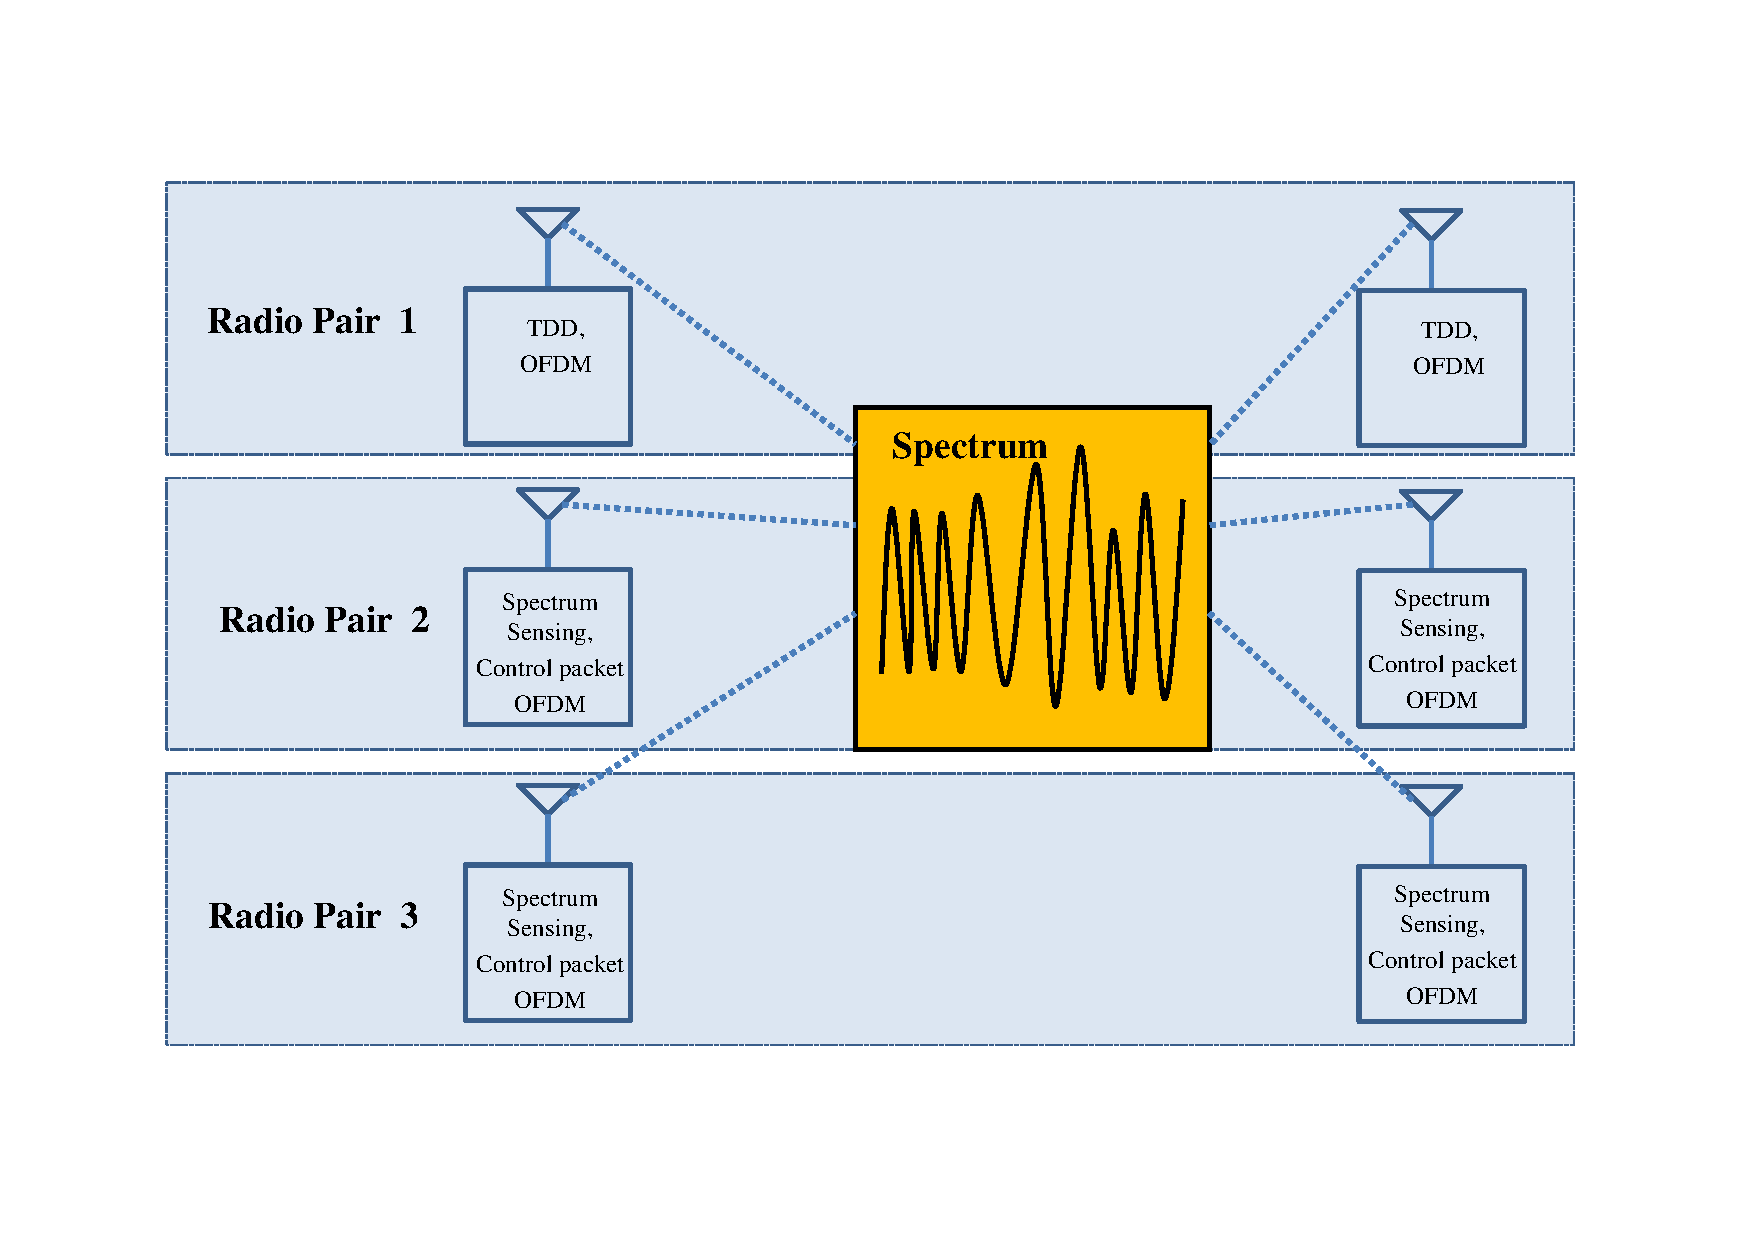
\includegraphics[width=160mm]{motivationExampleDSA.pdf}}
    \caption{Illustration of a distributed spectrum access system in which different types of radios try to share the same spectrum.}
    \label{fig:motivationExampleDSA}
  \end{center}
\end{figure}


This thesis focuses on both cooperative and competitive distributed spectrum access. In a cooperative distributed spectrum access system, standardized handshaking signals among all users could be used to achieve synchronization, depending on the application. For example, one user can claim to use part of the spectrum for a certain period of time by broadcasting an occupying or beacon signal, and all other users would avoid the spectrum occupied by the beacon signal and try to claim the right of another part of the spectrum. In this case, there should be a rule to enforce fair sharing of the spectrum. Otherwise, some greedy or malicious users can occupy the spectrum indefinitely. In other cases, handshaking signals are not used. For example, under severe conditions or extreme situations, such as natural disasters or accidents, it is desirable to have radios that can effectively and efficiently share the spectrum without direct coordination or spectrum preplanning. The FCC has designated a 700 MHz (698-806 MHz) frequency band for emergency use \cite{LLuYLi2012}.

In a competitive distributed spectrum access system, two or more users try to utilize the spectrum as much as possible. At the same time, each user interferes with other users, requiring robust signaling formats and often lower effective data rates and lower spectral efficiency. The objective of maximizing one��s own throughput and the objective of minimizing the throughput of competitors are usually consistent with each other. For instance, maximizing the transmission signal power has the potential not only to increase its own throughout but also to decrease competitors' throughout.

There is usually a power constraint for each user. Algorithms on the distribution of power across the spectrum need to be explored in terms of information theory and practical applications. There is a big gap between the information theory and the practical applications when developing power assignment algorithms. For example, in information theory, power can be assigned arbitrarily across frequency, but power assignment in practical application is limited by many factors, such as power amplifiers and modulation methods.

The Defense Advanced Research Projects Agency (DARPA) has initialized a program called the DARPA Spectrum Challenge to seek robust communications in a communication channel with unknown interfering signals \cite{DARPASpectrumChallenge}. The DARPA Spectrum Challenge consists of a cooperative competition and a competitive competition. The cooperative competition is a case of cooperative distributed spectrum access without standardized handshaking signal. The competitive competition is a case of competitive distributed spectrum access. In both competitions, each user has no prior knowledge of the other users.

\section{Scope and Contributions}
This thesis is motivated by the DARPA Spectrum Challenge. Theoretical analysis is conducted, and practical radios are designed and implemented with the GNU Radio software and the Ettus Universal Software Radio Peripheral (USRP) hardware. The radio design is subject to the constraints of the DARPA Spectrum Challenge.

The primary contribution of this thesis is to design and implement both a cooperative and a competitive radio for the DARPA Spectrum Challenge. The rules are analyzed, and strategies for both cooperative and competitive radio are developed. For both cooperative and competitive radios, a feedback scheme is analyzed based on the opportunities and limitation of the games, and a packet management system is implemented. For the cooperative radio, we developed a spectrum sensing technique based on statistics of the received energy across frequency. For the competitive radio, a time division duplex (TDD) system is developed. Many of these system components are likely to be useful beyond the DARPA Spectrum Challenge.

This thesis is organized as follows. Chapter \ref{chap:backgound} summarizes background on experimental wireless research using software-defined radio (SDR) as well as distributed spectrum access. Chapter \ref{chap:strategy} introduces the strategies for both competitive and cooperative matches, and Chapter \ref{chap:strategyAnalysis} analyzes the competitive and cooperative feedback strategies based on the rules. In Chapter \ref{chap:spectrumAnalysis}, a software spectrum sensor is designed. Chapter \ref{chap:TDD} introduces the design and implementation of a TDD system for the competitive radio. Chapter \ref{chap:performance} shows the test results and finally the conclusions and future work are summarized in Chapter \ref{chap:conclusion}.




%
% Chapter 2
%

\chapter{BACKGROUND}
\label{chap:backgound}
This chapter gives a brief summary of related research on spectrum sharing, software defined radio (SDR) tools, the DARPA Spectrum Challenge, and the physical-layer foundation for radio designs.


\section{Related Research on Spectrum Sharing}

Game theory applications of wireless networks from a layered perspective are summarized in \cite{DimitrisECharilasAthanasiosDPanagopoulos:2010}, which discusses game theory in the physical layer, data link layer, network layer and transport layer. In physical layer game theory, power control, spectrum allocation, multiple-input multiple output (MIMO) systems and cooperative communications are highlighted.

A cooperative game for distributed spectrum sharing is studied in \cite {JuanESurisLuizADaSilvaZhuHanandAllenBMacKenzie2007}. According to this model, the available bandwidth is divided equally into multiple channels. Each transmitter can transmit in any combination of channels at any time and can set its transmit power on each channel. Receiver nodes are not considered in the game. A distributed algorithm based on the Nash Bargaining Solution is proposed. However, some practical issues, such as synchronization and feedback between the transmitter and receiver, are not considered.

Power control for spectrum sharing in an unlicensed band, in which multiple systems coexist and interfere with each other, is studied in \cite{REtkinandAParekhandDTse2007}. Consider an $M$-user Gaussian interference channel in discrete time. From an information-theoretic perspective, the best power control strategy for a given system in the competitive game for each user is to spread its available power over the entire bandwidth using the water filling method. This solution assumes that the users can accurately estimate the interference environment in which they are operating.

This thesis takes inspiration from these theoretical works, but specifically addresses important mechanisms for synchronization, feedback, and learning the interference environment.



\section{Software-Defined Radio (SDR) Tools}
Our radio is implemented with the GNU Radio 3.7.2 software \cite{GNURadio} and the USRP N210 hardware from Ettus Research \cite{EttusResearch}. GNU Radio is a free and open-source software development toolkit that provides signal processing blocks to implement software radios. It can be used with external RF hardware to create software-defined radios, or without hardware in a simulation-like environment. GNU Radio applications are written in C++ and Python. The signal processing blocks are implemented in C++, which can then be connected together in Python to form a flow graph to process data in a streaming fashion.
\begin{figure}[tpb]
  \begin{center}
    \centerline{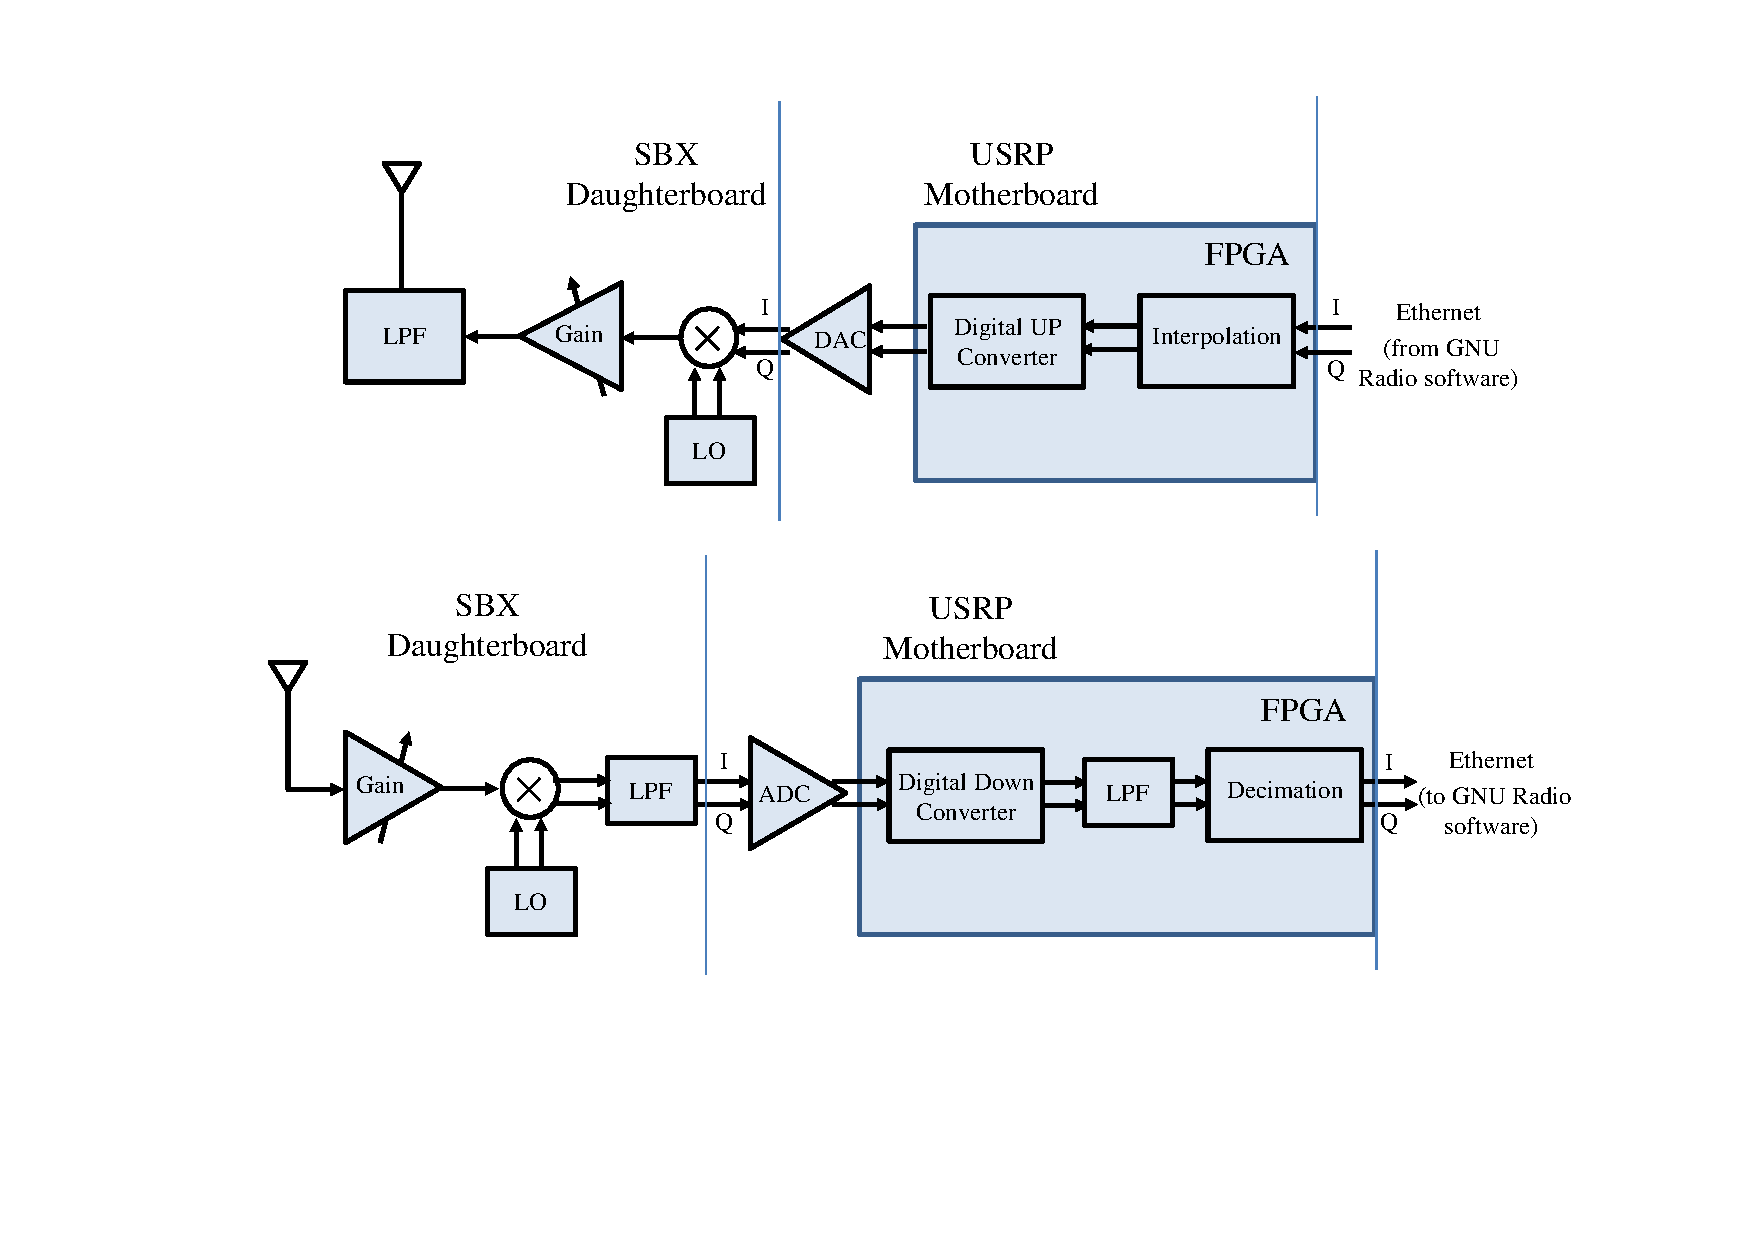
\includegraphics[width=180mm]{USRPandSBX.pdf}}
    \caption{Block diagram of the key components on the USRP N210 motherboard and the SBX daughter board.}
    \label{fig:USRPandSBX}
  \end{center}
\end{figure}


Figure~\ref{fig:USRPandSBX} shows the structure of the USRP N210 mother board and SBX daughter board. Ethernet connects the USRP to a computer running a GNU Radio program.


\section{The Spectrum Challenge}
Radios can often interfere with other radios and disrupt the operations. The DARPA Spectrum Challenge is a competition initiated in January 2013 to demonstrate a radio protocol that can best use a given communication channel in the presence of other dynamic users and interfering signals. The Challenge focuses on finding strategies instead of developing new radio hardware to guarantee robust wireless communication in congested electromagnetic environments \cite{DARPASpectrumChallenge}.

There are also other factors that motivate the need for distributed spectrum sharing. In rapid response operations, such as disaster relief, multiple radios come to the same geographic region and may try to use the same spectrum. It is desirable for the radios to efficiently share the spectrum without prior coordination. In the military and civilian sectors, high priority radios are required to operate regardless of the electromagnetic interference, to guarantee reliable communications and to avoid potential loss of life. Corresponding to these two needs, two matches were created in the Challenge: the cooperative match and the competitive match. Eighteen teams competed in the competitive match and the cooperative match in the Final Tournament.

\subsection{Challenge Rules}

The Spectrum Challenge uses the ORBIT test bed for design development, practice sessions, and tournaments \cite{OrbitLab}. It has implemented a SDR platform consisting of computers and USRP N210s. Teams may use any software development tools and programming languages, but no modifications of the test bed hardware is permitted. The final design must run on the ORBIT test bed by simply loading an image and executing a single console command.

All radios must be designed to operate within a limited bandwidth. The allowable bandwidth is controlled by two parameters: the specified RF center frequency of the band, denoted $F_c$, and the maximum sampling rate of the USRP, denoted $R_{max}$. In the Final Challenge event, $F_c=600$ MHz, and $R_{max}=5$ million samples per second for both the transmitter and receiver. The allowable frequency band is therefore given by
\begin{align}
F_c - R_{max}/2 \le f \le F_c + R_{max}/2.
\end{align}
This constraint does not imply that the radio's carrier frequency must be set to be $F_c$, nor does it require the sampling rate to be $R_{max}$ at all times. However, the allowable bandwidth for the transmitter and receiver is restricted by the maximum sample rate and the specified center frequency $f$ by
\begin{align}
&f+\frac{r}{2} \le F_c + R_{max}/2&\\
&f-\frac{r}{2} \ge F_c - R_{max}/2,&
\end{align}
where $r$ is the user-programmed sampling rate. The radio could transmit anywhere within the actual bandwidth limitation as long as the chosen carrier frequency and sampling rate satisfy the above limits.

The total transmission power is not limited, but it is restricted by the hardware, USRP N210. Since every team uses the same type of hardware, the maximum achievable transmission power can be assumed to be the same for each team. The actual transmission power of each team depends on their radio design.

In both competitive and cooperative games, one radio node in each pair draws packets from the server and the other delivers packets back to the server. Drawn and delivered packet sizes are fixed at 1440 bytes and the total file size, i.e., total number of packets ($D$) is 15000.

\subsubsection{Radio Geometry and ORBIT Grid Configuration}
Figure~\ref{fig:CooperativeNodeAssignement} shows the radio node geometry for the cooperative match. There are three teams in each cooperative game. The source and destination nodes are labeled by S and D, respectively. The source node requests data packets from the server, and the destination node returns data packets to the server. The goal is to transmit data packets from the source to the destination.

The distance $R_1$ from the source to destination is roughly 76 feet, and the distances $R_2$ between source nodes (S1-S3 and S2-S3 ) and between destination nodes (D1-D3 and D2-D3) is roughly 3 feet.

\begin{figure}[tpb]
  \begin{center}
    \centerline{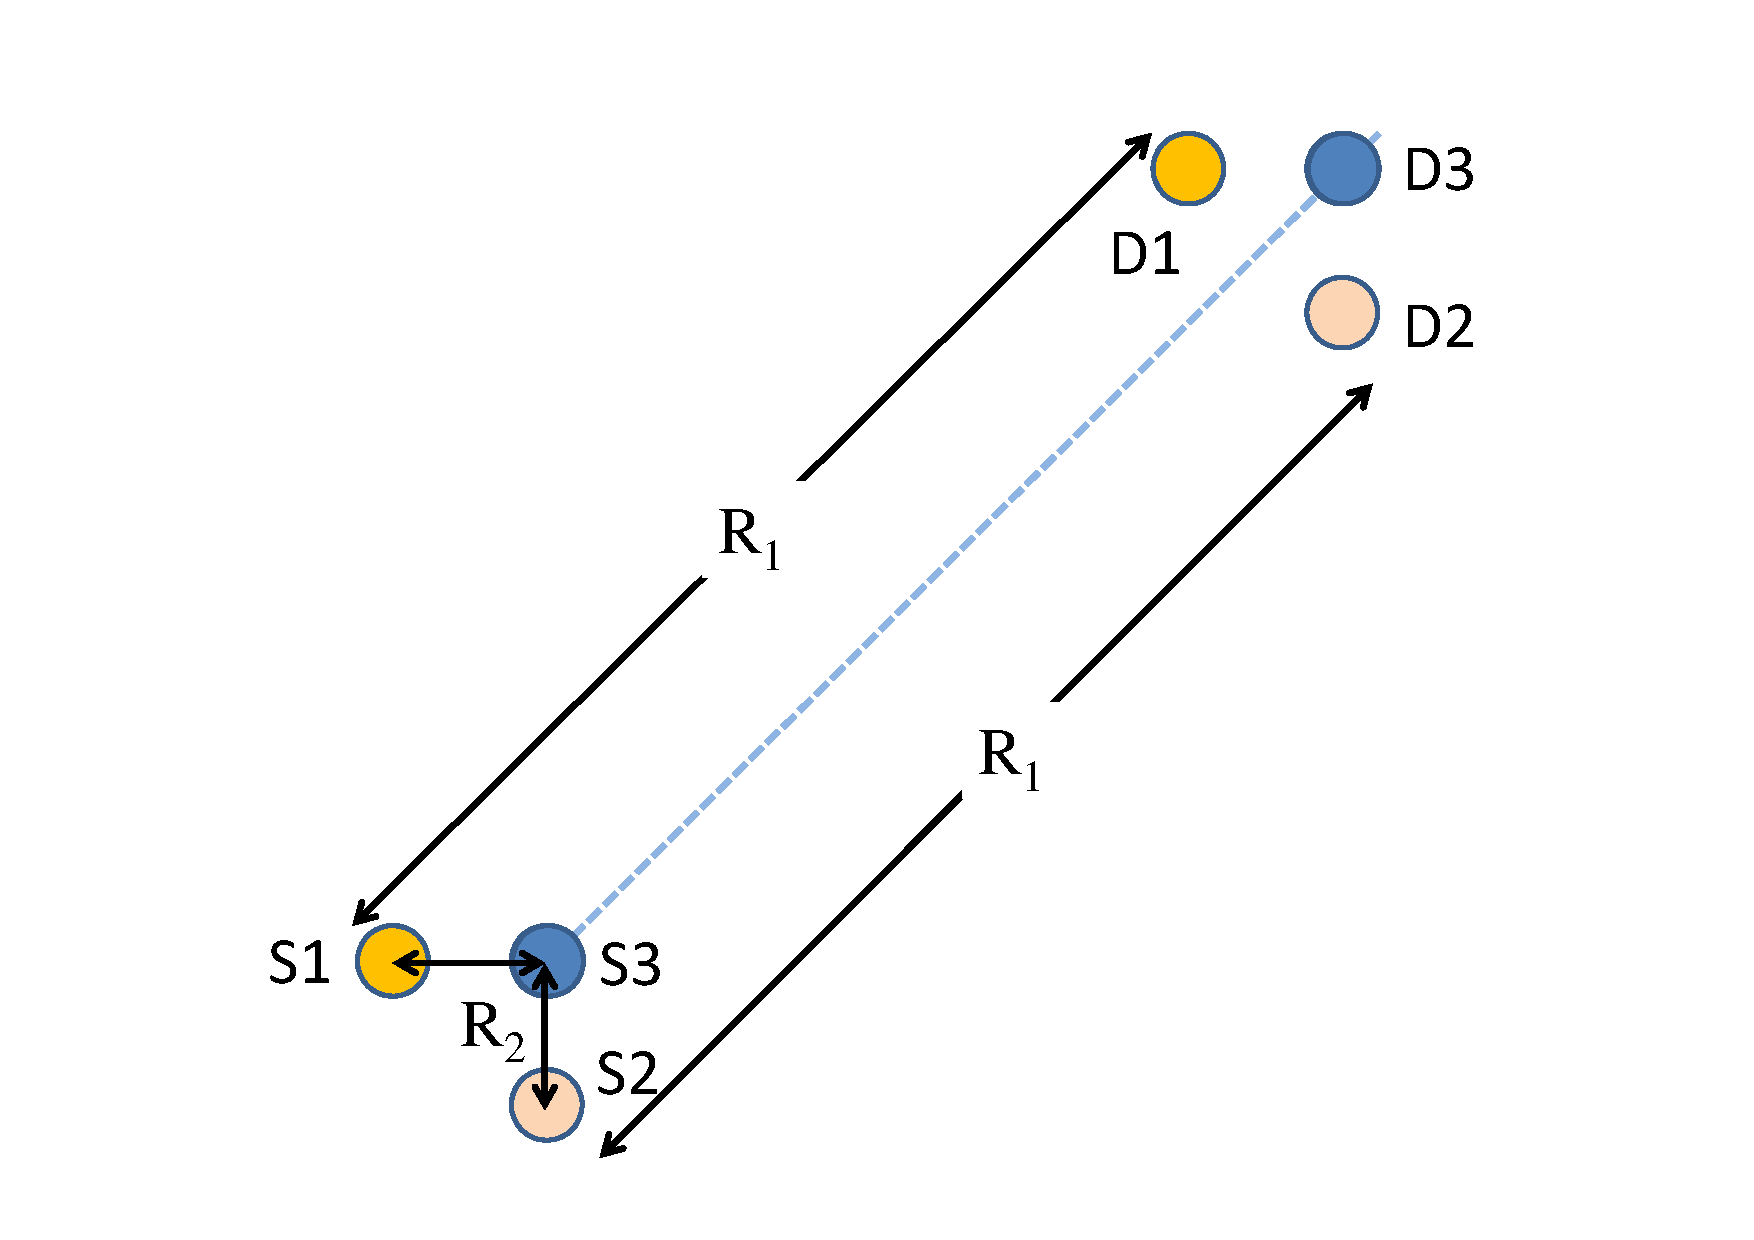
\includegraphics[width=150mm]{CooperativeNodeAssignement.pdf}}
    \caption{Radio node geometry for the cooperative match. The distances are roughly $R_1=76$ feet and $R_2=3$ feet.}
    \label{fig:CooperativeNodeAssignement}
  \end{center}
\end{figure}

Figure~\ref{fig:CompetitiveNodeGeometryFinalRound} shows the radio node geometry for the competitive match. There are two teams competing with each other in each competitive game and they are represented by different colors. The distances $R$ R between nodes in the pairs S1-D1, S2-D2 and D1-D2 is roughly $R=$ 25 feet.
\begin{figure}[tpb]
  \begin{center}
    \centerline{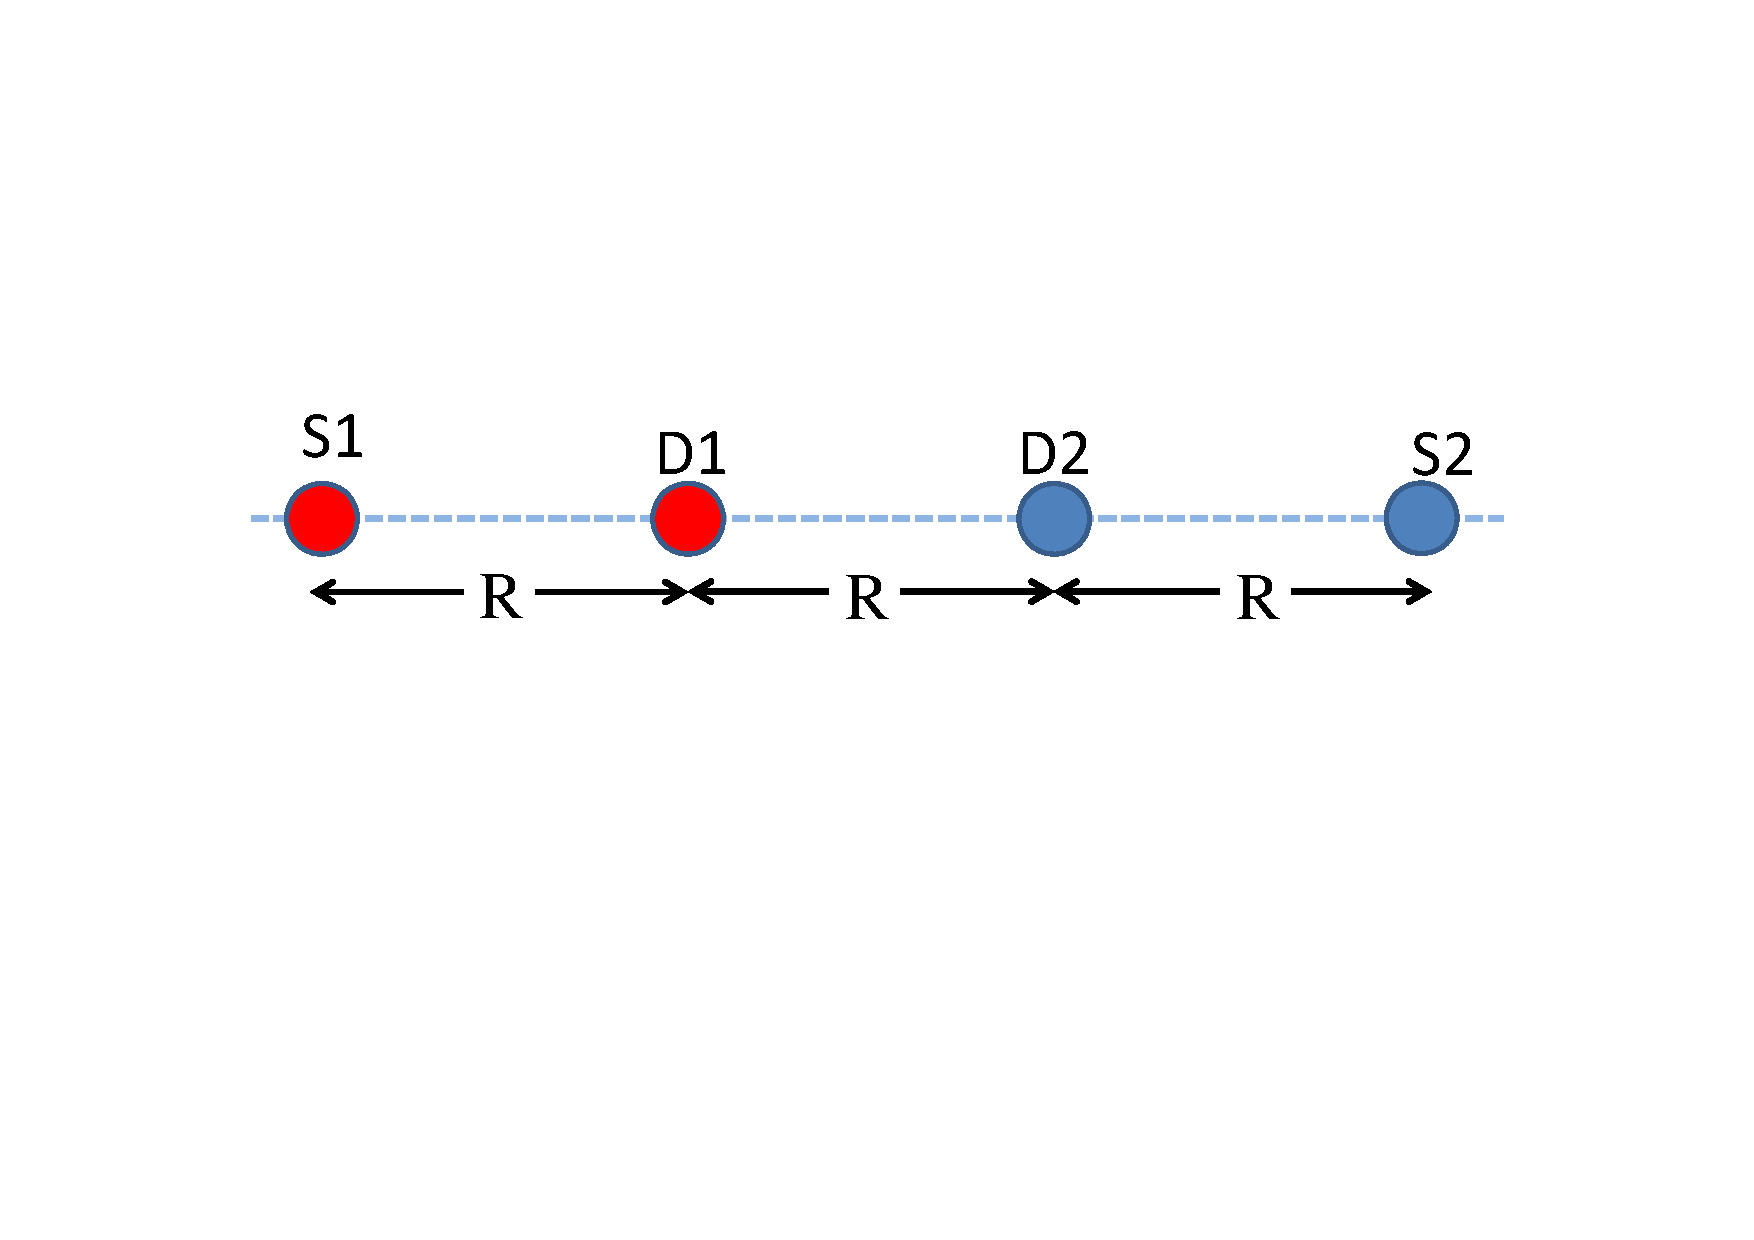
\includegraphics[width=150mm]{CompetitiveNodeGeometryFinalRound.pdf}}
    \caption{Radio node geometry for competitive match. The distances are roughly $R=25$ feet.}
    \label{fig:CompetitiveNodeGeometryFinalRound}
  \end{center}
\end{figure}

A match consists of two games such that a team plays one game using the S1/D1 pair and the other game using the S2/D2 pair. Each team's score for a match is the sum of its successful packets transferred in both games.

\subsection{Cooperative Tournament}
The tournament structure consisting of a number of matches among three teams is depicted in Figure~\ref{fig:CooperativeTournamentStructure}. The three rounds are the preliminary round, semifinal round and final round. The score of each team in one round is not counted in other rounds.

\begin{figure}[tpb]
  \begin{center}
    \centerline{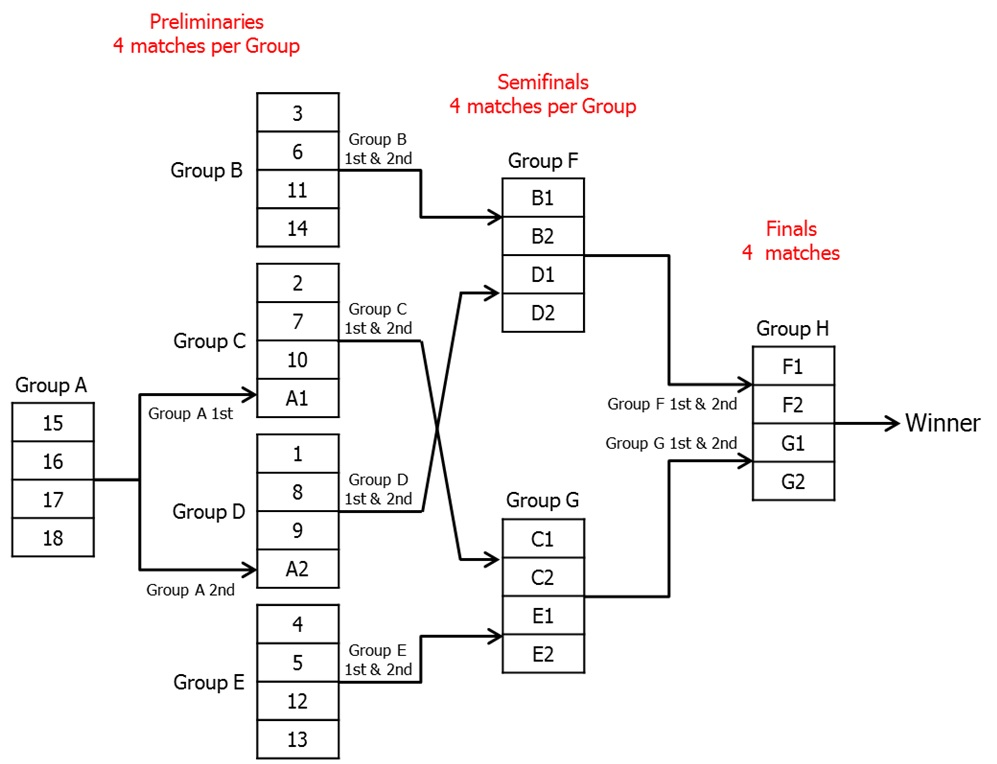
\includegraphics[width=170mm]{CooperativeTournamentStructure.jpg}}
    \caption{Cooperative Tournament Structure}
    \label{fig:CooperativeTournamentStructure}
  \end{center}
\end{figure}

The cooperative game ends (at time $t$) once all three radio pairs have successfully transmitted all of their data or once the maximum time ($T = 3$) minutes is reached. Suppose that $X_i$ ($i=1,2,3$) denotes the number of packets successfully transferred for team $i$. Sort $X_i$ in descending order to get $Y_1$, $Y_2$ and $Y_3$. The score for team $i$ is
\begin{align}
{S_i} = {X_i} + {Y_1} + {Y_2}, \quad i=1,2,3.
\end{align}
This scoring scheme encourages each team to be aggressive in the cooperative game.

In the preliminary round, 18 teams are divided into 5 groups of 4 (Groups A to E). One spot in each of Groups C and D is filled with the top two teams from Group A. Within each group, games are played among all combinations of 3 teams, resulting in 3 games per team. A team's match score is the sum of its 3 game scores in the current round. The 2 teams with the highest match scores from Groups B and C advance to the semifinal round as Group F. The 2 teams with the highest match score from Groups D and E advance as Group G.

In the semifinal round, the 2 groups of 4 teams (Groups F and G) play all combinations of 3 teams, with three games in each match to average out radio configurations as in earlier rounds, and each team accumulates a match score from its 3 games. The first and second highest scoring teams from each group advance to the final round.

In the final round, the 4 remaining teams play in all combinations of 4 and accumulate a score from their 4 matches. The winner is the team with the highest match score in the final round.


\subsection{Competitive Tournament}
The tournament structure is depicted in Figure~\ref{fig:CompetitiveTournamentStructure}. The three rounds are the preliminary round, semifinal round and final round. The score of each team in one round is not counted in other rounds.
\begin{figure}[tpb]
  \begin{center}
    \centerline{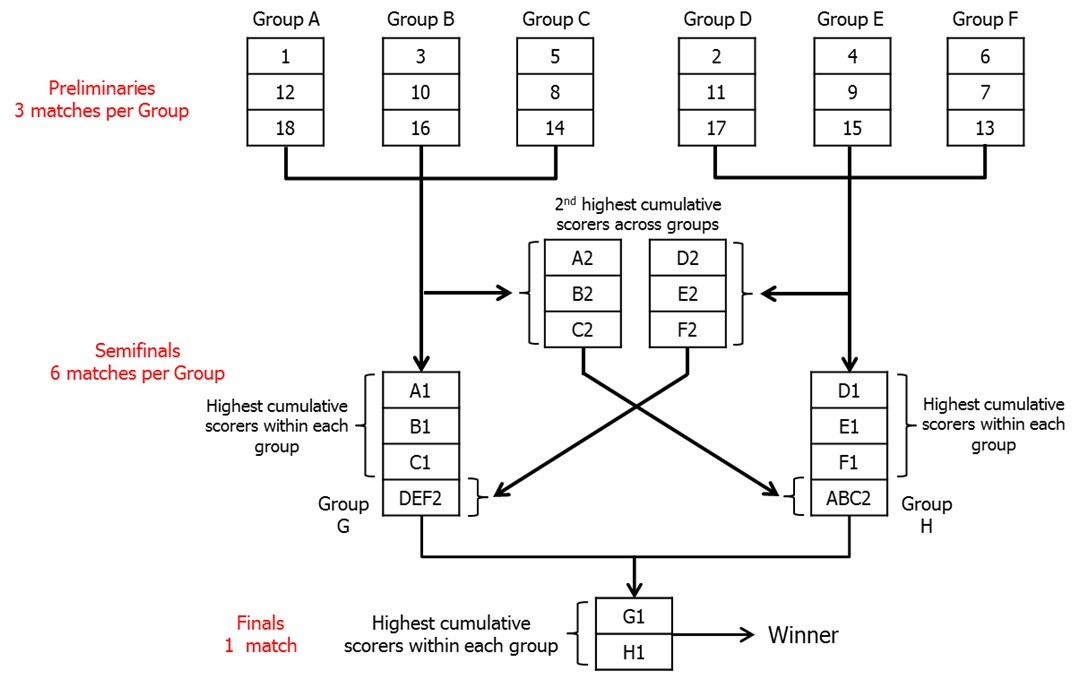
\includegraphics[width=170mm]{CompetitiveTournamentStructure.jpg}}
    \caption{Competitive Tournament Structure}
    \label{fig:CompetitiveTournamentStructure}
  \end{center}
\end{figure}

In the preliminary round, the 18 teams are divided into 6 groups of 3 (Group A to F). Within each group, matches are played between all pairs of teams, providing 2 games per team. A team's match score is the sum of the 2 game scores, i.e., the total number of packets successfully transferred. In a game, a team completes a trial using the S1/D1 nodes and another trial using the S2/D2 nodes. The team with the highest match scores across the games played within each group advances to the semifinals. The teams with the second highest scores in Group A, B, and C are designated A2, B2, and C2 in Figure~\ref{fig:CompetitiveTournamentStructure}. Teams A2, B2, and C2 play all combinations (2 games per team), and the team with the highest cumulative score advances to the semifinals as team ABC2. Similarly, the teams with the second highest scores in Groups D, E, and F(D2, E2, and F2) play all combinations and the team with the highest cumulative score advance as team DEF2

In the semifinal round, the 2 groups of 4 teams (Groups G and H) play all combinations. Each team accumulates a score from its 6 games. The teams with the highest scores within each group advance to the final round.

The final round consists of 1 match, again of two trials to account for radio variations, to determine the overall winner.

\section{Preliminary Analysis}
Preliminary analysis is conducted based on the radio geometries and game metrics. Many of these aspects will be discussed and designed in details in later chapters.
\subsection{Preliminary Cooperative Analysis}
Our radio should avoid conflicting with other teams in frequency. In the Spectrum Challenge, no spectrum usage of other radios is disclosed in advance. Therefore, spectrum sensing is necessary to analyze the spectrum usage of other teams. From Figure \ref{fig:CooperativeNodeAssignement}, the sources are crowded together, which means that most of the signal energy from each radio is on the source side. As a result, the spectrum sensing should be done on the source side.

The reverse link (from destination to source) has low signal-to-interference ratio (SIR), and feedback seems to be impossible. However, if a narrow-band signal is used, the SIR can be significantly increased in that narrow band. Tests have demonstrated narrow-band feedback is achievable if the feedback signal is transmitted on the channel where no interference from other teams is present on the source side.

\subsection{Preliminary Competitive Analysis}
A good power control strategy for each team in the competitive game is to spread the available power over the entire bandwidth using the water filling method. Since equilibrium strategy for each team is to spread power evenly across the entire spectrum as discussed in \cite{REtkinandAParekhandDTse2007}, the strategy implemented in our radio should include such strategy.

From Figure~\ref{fig:CompetitiveNodeGeometryFinalRound}, the reverse link should have lower SIR than the forward link, and should be more reliable than the forward link. Therefore, feedback can be implemented to increase the throughput.

\section{Physical-Layer Foundation}
Orthogonal frequency-division multiplexing (OFDM) is used as the core modulation technique in our radio \cite{DingNieCompetitivePlan2013}. OFDM is chosen for several reasons. First the symbol rate can correspond to the maximum sampling rate of 5 MHz, whereas single-carrier modulation techniques require excess bandwidth and over-sampling. Second, OFDM is more flexible with multiple tones that can be used or not, which is significant in our competitive and cooperative strategies.

For both the cooperative radio and competitive radios, 512 tones are used, each with 9.77 kHz subcarrier spacing. We index the tones as tone $1,2,3,...,512$, from the lowest frequency to the highest frequency. A cyclic prefix (CP) with length of 8 samples is used in one OFDM symbol to allow for low-complexity estimation and equalization of multipath fading. The length for each OFDM symbol is 520 samples, or 104 $\mu s$.

We now highlight differences between the physical-layers of the cooperative radio and the competitive radio.

\subsection{Physical Layer Specification of the Cooperative Radio}
\label{coopPhysicalLayer}
An OFDM sub-frame consists of 1 symbol of preamble followed by 16 OFDM data symbols for a total of 17 OFDM symbols. The preamble is used to enable time and frequency synchronization as well as channel estimation at the receivers. In the frequency domain, the preamble is a set of pseudo-random sequences of -1, 0 and +1 known to both the source and destination, and the non-zero values appear every 8 tones except for the DC tone. The 512 OFDM tones are divided into 16 sub-bands as shown in Figure~\ref{fig:CoopPhysicalLayer}. Tones 1 to 13, tones 254 to 259 and tones 500 to 512 are not used because of the rolloff effect on the edge of 5 MHz and because of the DC offset around the DC tone. The unused tones correspond to a sort of 6.7$\%$ excess bandwidth. All the remaining 480 tones are divided evenly into 16 sub-bands and each sub-band has 30 tones. We index the sub-band as sub-band $1,2,...,16$ from lowest to highest frequencies. Each sub-band can be turned on and off separately, including the preamble in that sub-band.

In the time domain, the preamble symbol has 8.125 identical repetitions during 104$\mu s$. This repetition feature helps the receiver to identify the preamble and acquire OFDM synchronization. In the cooperative radio, preambles are also used as pilots to do channel estimation in the 5 MHz bandwidth. In the frequency domain, the non-zero symbols are placed every 8 tones. Based upon measurements using the ORBIT testbed, the channel appears quite flat, so averaging can be performed across frequency when estimating the channel.

\begin{figure}[tpb]
  \begin{center}
    \centerline{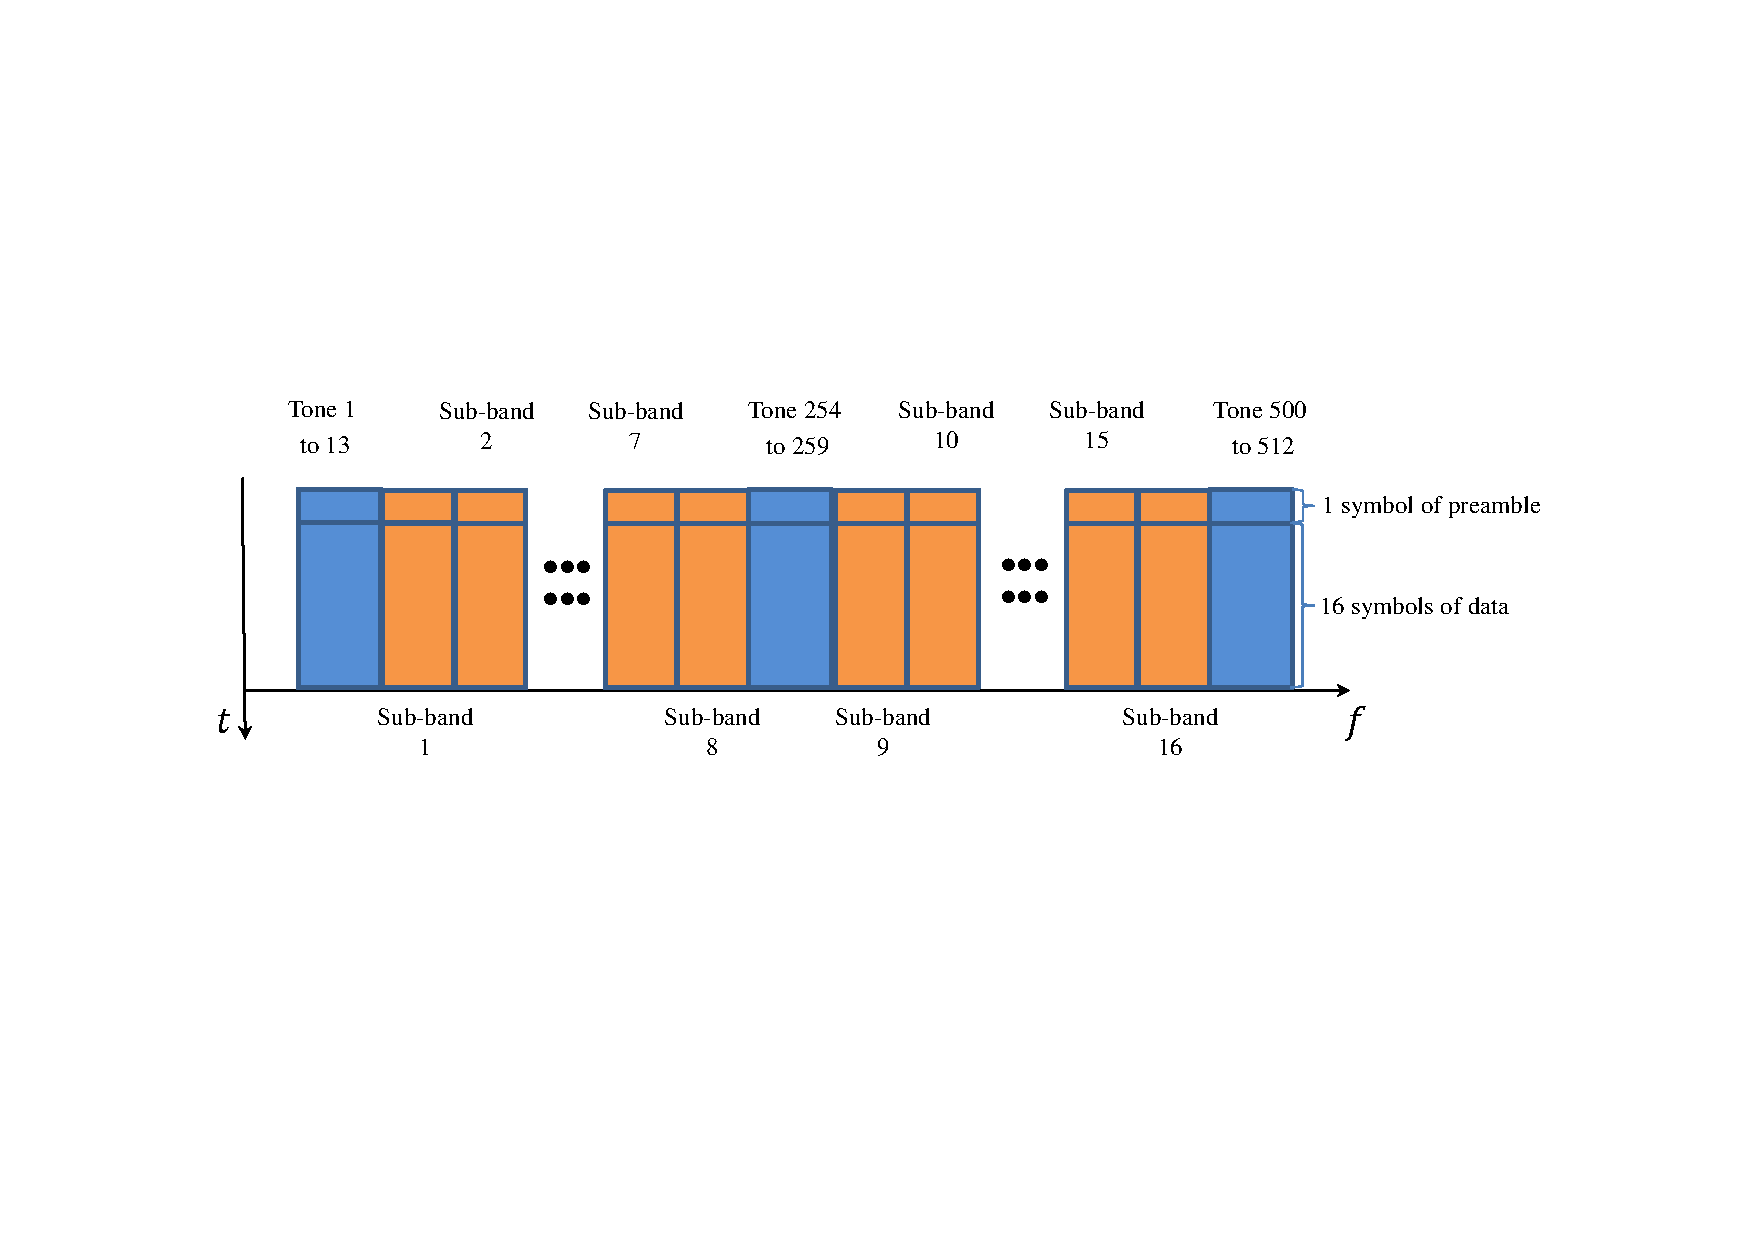
\includegraphics[width=160mm]{CoopPhysicalLayer.pdf}}
    \caption{OFDM specifications for the cooperative radio. The darker color indicates unused sub-bands, and the lighter color indicates used sub-bands.}
    \label{fig:CoopPhysicalLayer}
  \end{center}
\end{figure}

\subsection{Physical Layer Specification of the Competitive Radio}
An OFDM sub-frame consists of 1 symbol of preamble followed by 1 symbol of pilot and 16 OFDM data symbols for a total of 18 OFDM symbols. In the frequency domain, the non-zero values of the preamble appear every 2 tones except for the DC tone, and the non-zero values of pilot are placed every 8 tones except for the DC tone. The 512 OFDM tones are divided into 8 sub-bands as shown in Figure~\ref{fig:CompPhysicalLayer}. Tones 1 to 13, tones 254 to 259 and tones 500 to 512 are not used similar to the cooperative radio. All the remaining 480 tones are divided evenly into 8 sub-bands, with each sub-band having 60 tones. We index the sub-band as sub-bands $1,2,...,8$ from lowest to highest frequencies. The data OFDM symbols of each sub-band can be turned on and off separately, but the preamble and pilot symbols are always generated.

\begin{figure}[tpb]
  \begin{center}
    \centerline{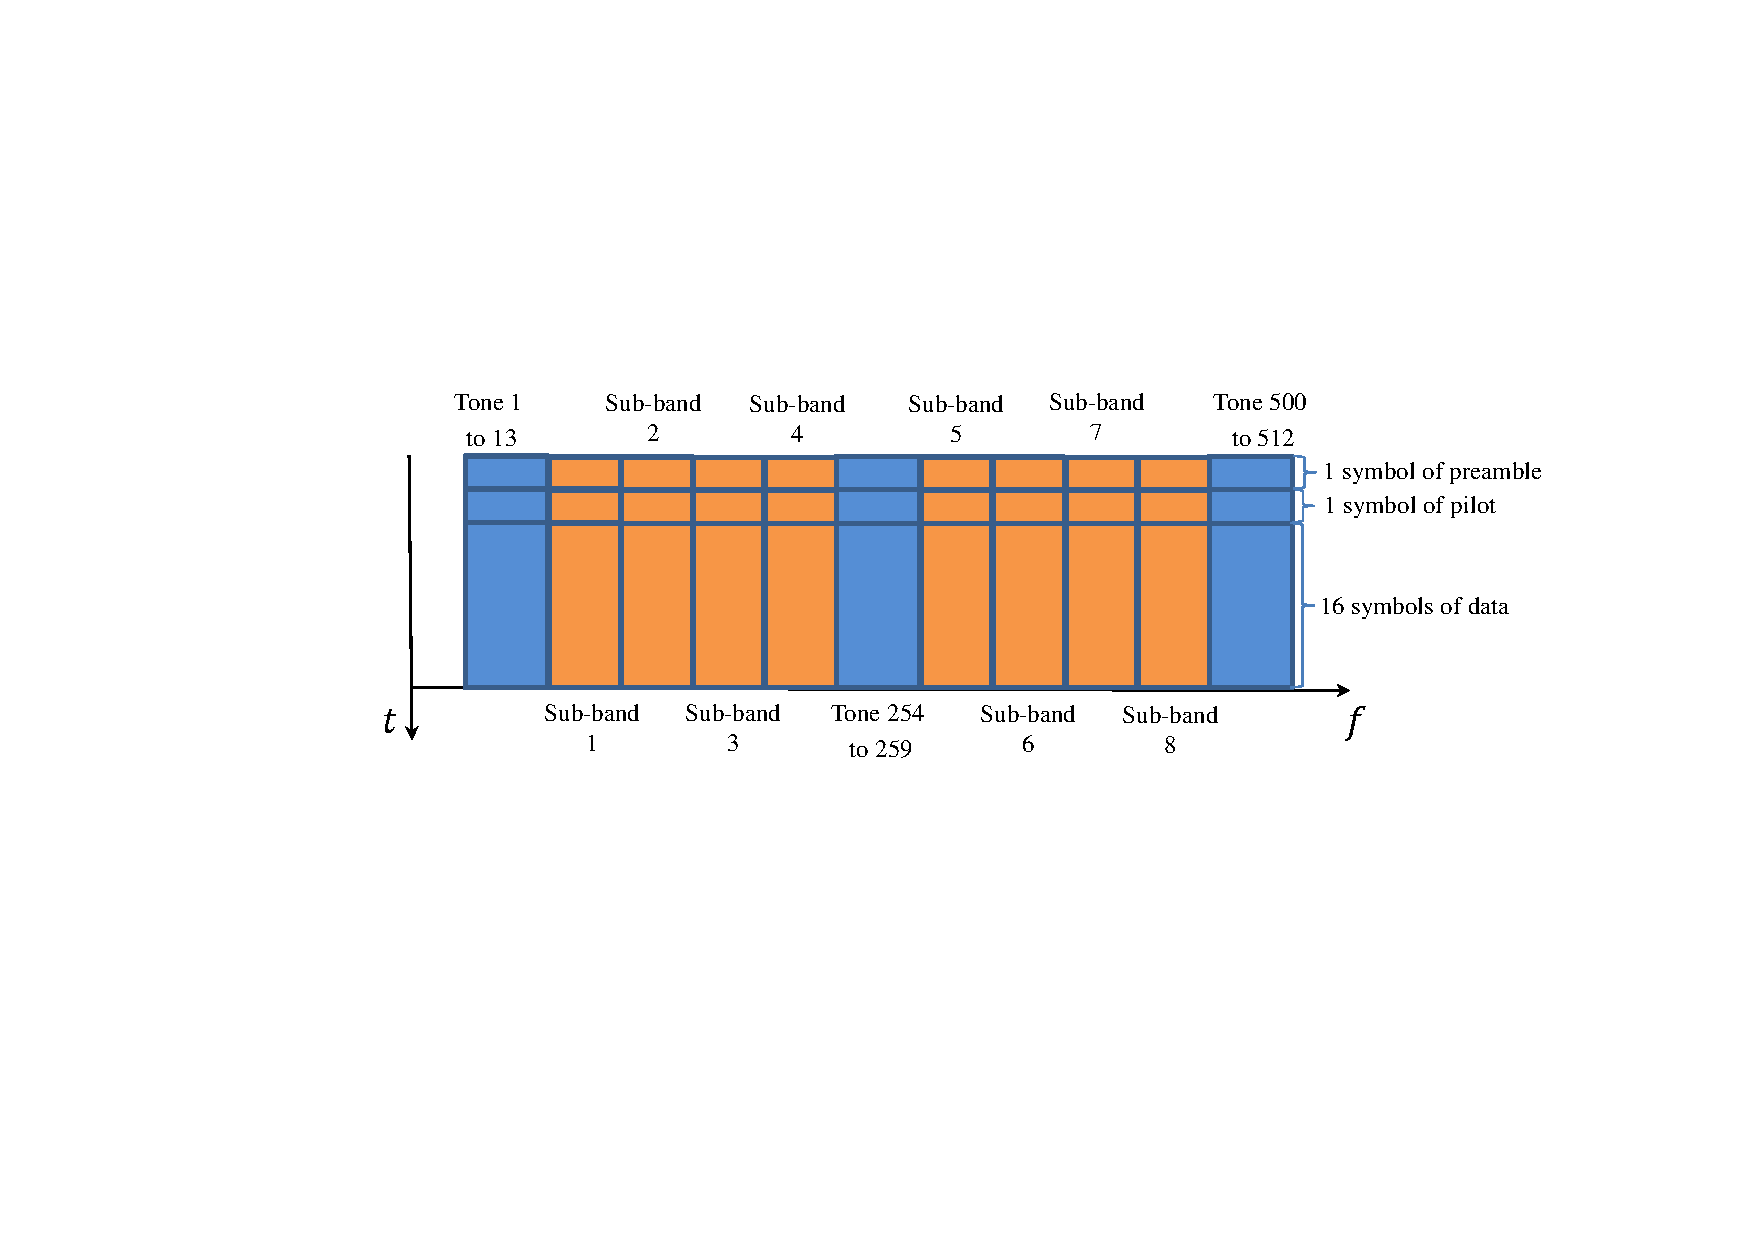
\includegraphics[width=160mm]{CompPhysicalLayer.pdf}}
    \caption{OFDM specifications for the competitive radio. The darker color indicates unused sub-bands, and the lighter color indicates used sub-bands.}
    \label{fig:CompPhysicalLayer}
  \end{center}
\end{figure}



%%%%%%%%%%%%%%%%%%%%%%%%%%%%%%%%%%%%%%%%%%%%%%%%%%%%%%%%%%%%%%%%%%%%%%%%
%
% Chapter 3
%

\chapter{DESIGN OF GAME STRATEGIES}
\label{chap:strategy}
The analysis and design of game strategies in this project were a team effort, that incorporated ideas from former works in \cite{FanZhang2013, MingmingCai2013, ChaoLuo2013}. My contribution in this chapter includes developing the cooperative strategy, and improving the competitive strategy.


\section{Cooperative Strategy}
In the cooperative game, we want to maximize the throughput for all the radios in a group. Consequently, our radio should avoid transmitting on parts of the band that other teams are using. Since no prior knowledge of other radios can be used, a spectrum analyzer to sense the usage of the spectrum was chosen based on the topology of the radios as shown in Figure \ref{fig:CooperativeNodeAssignement}. Since most of the signal energy from each radio is on the source side, spectrum sensing on the source side will result in better accuracy.

In most papers discussing spectrum sharing, the synchronization between the source and destination is not considered. However, in a real pair of radios, if the destination does not know which sub-bands are used, it cannot apply an appropriate filter to reduce interference. In our design, a state machine is used to synchronize the source and destination, which has been successfully developed in \cite{FanZhang2013}. The state machine packs the decision into a control packet, and then transmits the control packet to the receiver with 200 kHz-bandwidth and a 64-tone OFDM signal in four different center frequencies across the 5 MHz bandwidth. The limited energy is focused in a very narrow band, and the state machine's signal has very high SIR. Tests show that the state machine is reliable. Technical details on the state machine can be found in \cite{FanZhang2013}.

Feedback can significantly improve the radio performance, and it is also part of our cooperative radio design. Like the state machine, a narrow-band signal is used to increase the SIR. Detailed information on the feedback is discussed in Chapter \ref{chap:strategyAnalysis}.

Figures~\ref{fig:CooperativeStrategy} and \ref{fig:CooperativeCycle} shows the high level algorithm. The four states of the algorithm are spectrum sensing, control packet, feedback, and data transmission. More details on the spectrum sensing is studied in Chapter \ref{chap:spectrumAnalysis}.

\begin{figure}[tpb]
  \begin{center}
    \centerline{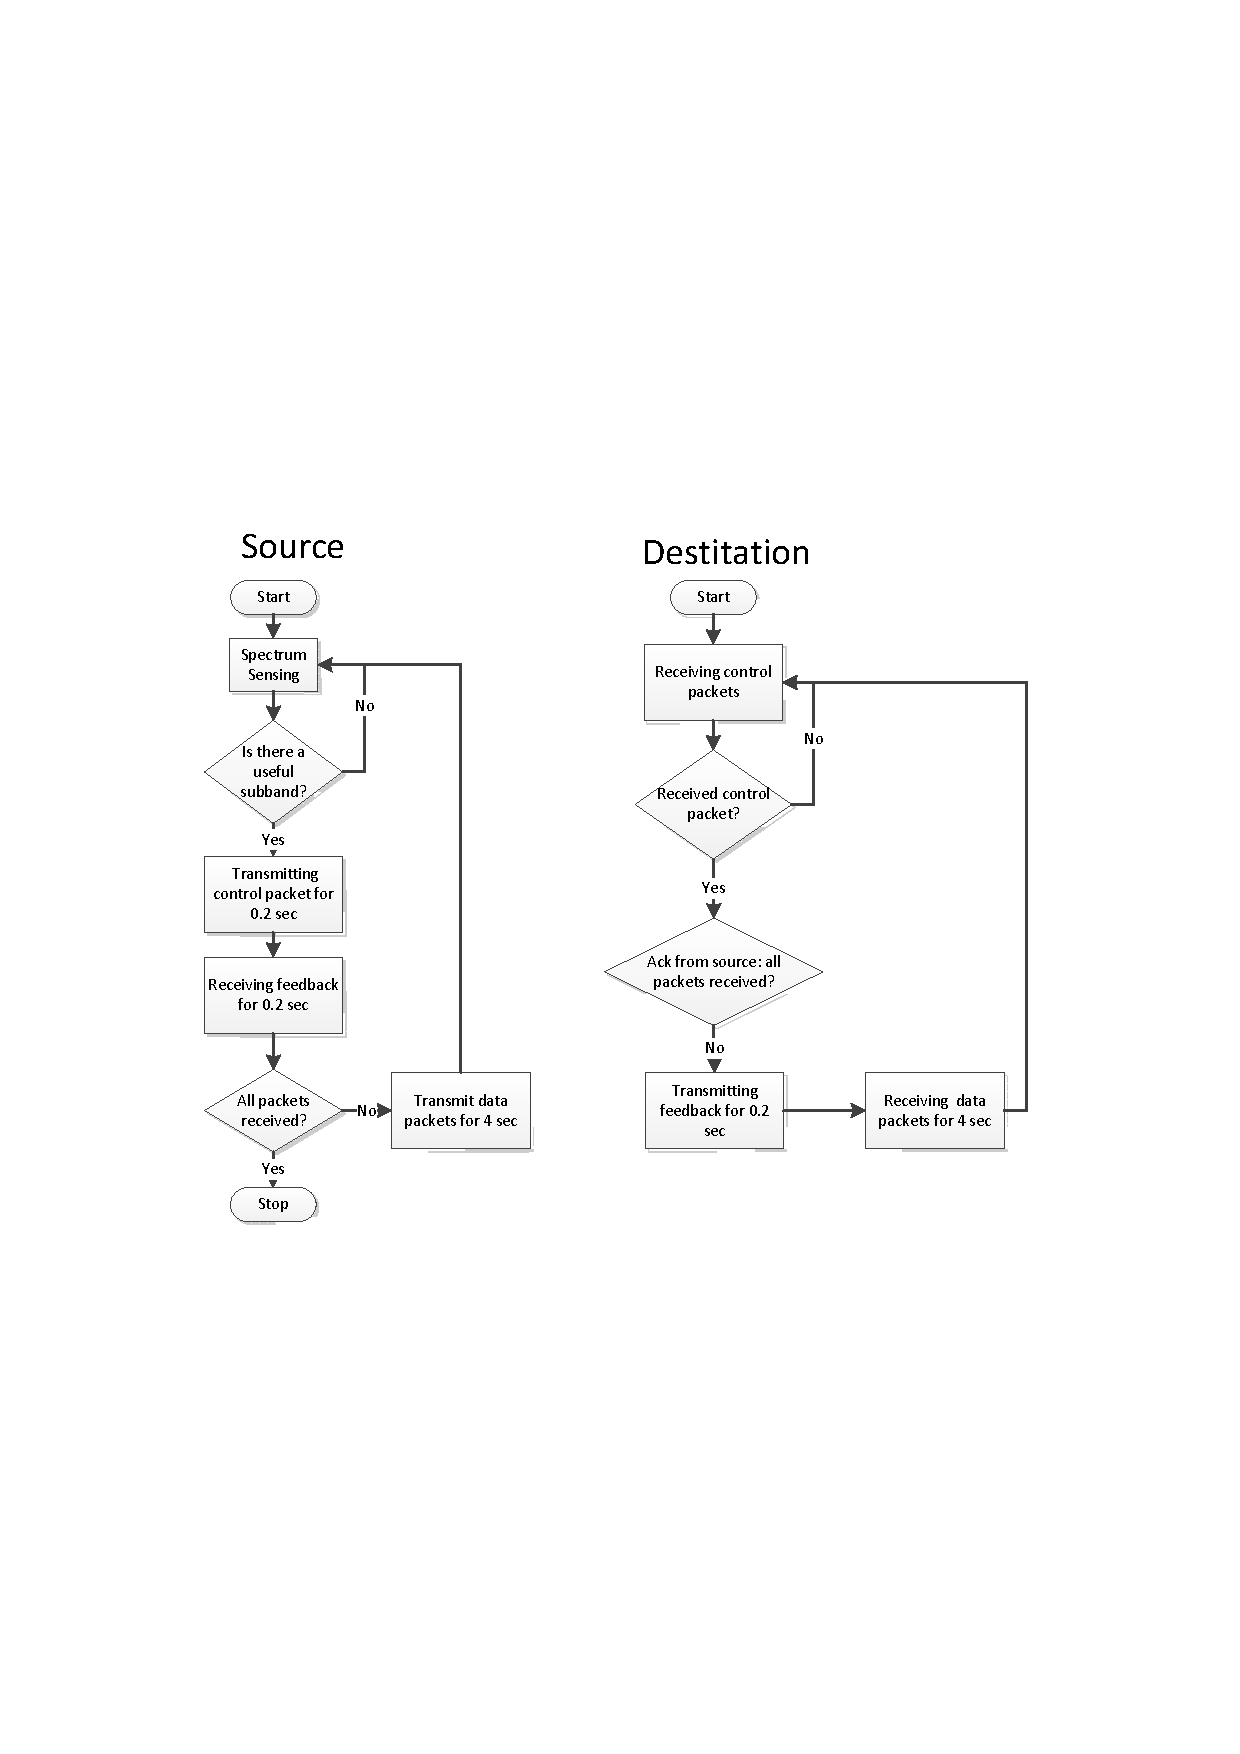
\includegraphics[width=160mm]{CooperativeStrategy.pdf}}
    \caption{Cooperative Strategy}
    \label{fig:CooperativeStrategy}
  \end{center}
\end{figure}

In the control packet state, the source sends 125 control packets, each with same content, through 200 kHz OFDM signal. Each packet has a duration of about 1.8 $ms$. Once the destination receives one of the control packets, it moves to the next state.

In the feedback state, the destination sends feedback packets. From the spectrum sensing results, the center frequency is determined to be the band that has the lowest interference. Both the source and destination choose the largest available band to transmit the feedback packet.

In the data transmission state, 512 tones are divided into 16 sub-bands, each containing 30 tones as discussed in Section \ref{coopPhysicalLayer}. Each sub-band transmits one physical-layer packet. The total data transmission time is about 4 seconds. The total non-data transmission time, including spectrum sensing, synchronization by the state machine, feedback, and switching time, is about 1 second.

In the GNU Radio software, a flow graph consists of the signal processing blocks and the connection among the blocks. Each flow graph needs hundreds of milliseconds to be constructed and also hundreds of milliseconds to be destroyed. Multiple flow graphs can exist in computer's memory at the same time, but only one can run in the CPU at a time. Switching among flow graphs can be achieved by locking the current running flow graph and then unlocking the flow graph to be run. Locking and unlocking the flow graphs requires a few milliseconds. The transmitter of the USRP can only accept one stream of data as input. Therefore, two blocks that output data to the same transmitter of the USRP cannot be implemented in the same flow graph. In our design of cooperative radio, multiple states need more than one flow graph. Ideally, each state should be implemented in one flow graph to modularize the program. As a result, a smaller number of flow graphs is preferred. Finally, two flow graphs are used for both the source and destination. Figure~\ref{fig:CooperativeCycle} illustrates the process of one cooperative cycle, where the dotted box represents one flow graph. In order to reduce the switching time, switching between the flow graphs is conducted by locking and unlocking operation rather than by the construction and destruction of flow graphs.

\begin{figure}[tpb]
  \begin{center}
    \centerline{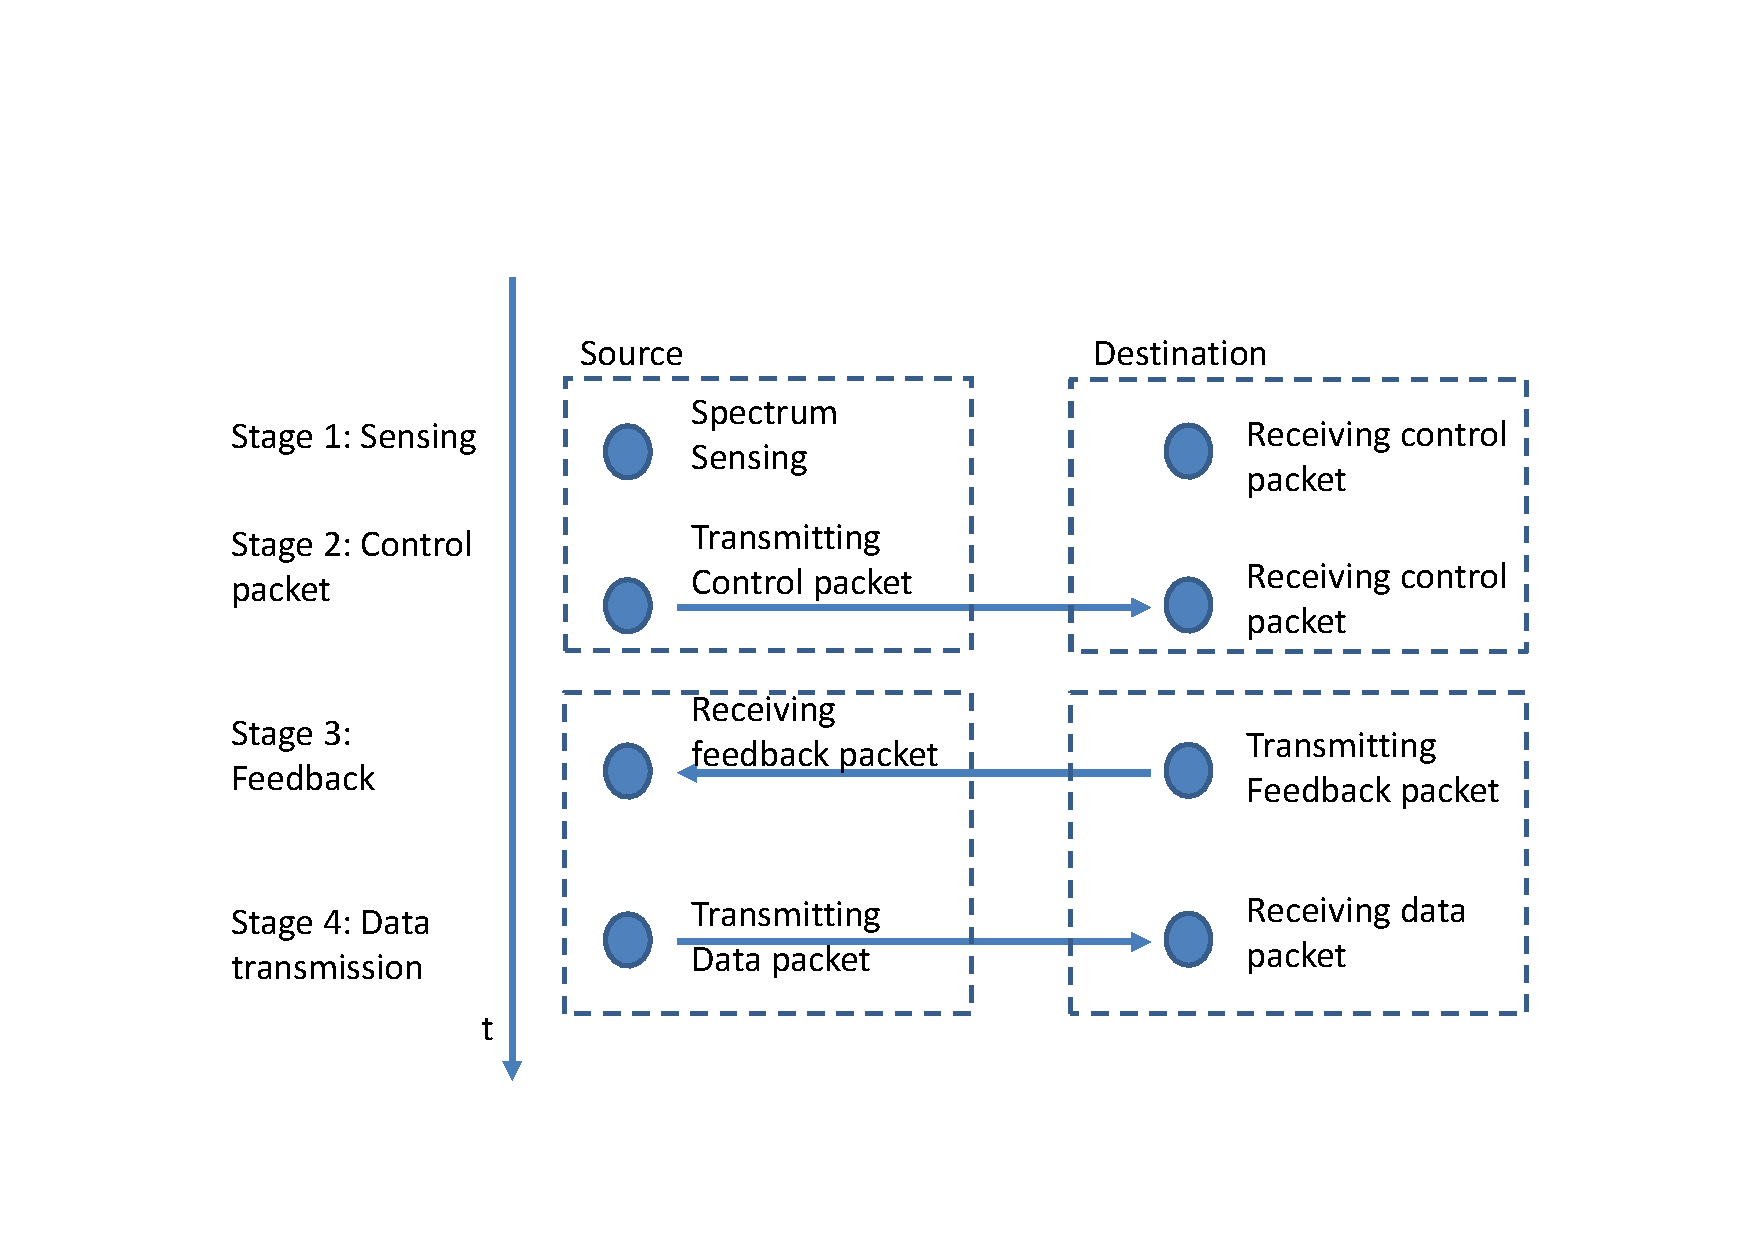
\includegraphics[width=160mm]{CooperativeCycle.pdf}}
    \caption{One Cooperative Cycle. The dotted boxes represent one flow graph.}
    \label{fig:CooperativeCycle}
  \end{center}
\end{figure}


\section{Competitive Strategy}
\label{comptititveStrategy}
In Figure~\ref{fig:CompetitiveNodeGeometryFinalRound}, S1 is farther away from the competitor nodes S2 and D2 than D1, so the reverse link is subject to less interference than the forward link. As a result, the reverse link is more reliable. Therefore, feedback can be applied to increase the reliability and efficiency of the forward link in the competitive match. Generally, the two ways to implement the feedback are time division duplex (TDD) and frequency division duplex (FDD).

In FDD systems, the forward and the reverse links occupy different frequency bands. In TDD systems, the forward and the reverse links share the spectrum with time multiplexing. FDD systems need a large guard band to ensure no interference between the forward link and the reverse link. However, we must take into account the close proximity of the transmitter and receiver antennas. A front-end filter would be needed to implement FDD, but no such front-end filter exists in USRP. If FDD is implemented with the USRP, the front-end amplifier will be saturated by the signal from the transmitter at the same USRP.

Consequently, TDD will be used to implement the feedback. The TDD sync can be controlled by either the source or destination. Since the reverse link is more reliable than the forward link, we let the destination node control the TDD sync by periodically sending the TDD preamble containing TDD sync information to the source. More details on TDD will be discussed in Chapter \ref{chap:TDD}.

We define a TDD frame as the transmission period of a TDD cycle. A TDD sub-frame is defined as a collection of data that is synchronized by one preamble in OFDM. In a TDD frame, 100 sub-frames will be sent through the forward link and 10 sub-frames will be sent through the reverse link. So our system keeps a 10:1 time ratio between the forward and reverse link. The time of each frame is 206 $ms$.

In both the forward link and reverse link, 512 subcarriers are divided into 8 sub-bands, each containing 60 subcarriers (the unused subcarriers are reserved for the DC tone and side lobes). We refer to the data transmitted in a sub-band of a sub-frame as a physical-layer packet, and its size is 256 bytes if QPSK is used. A 32-bit CRC check is attached to each physical-layer packet.

Channel coding is used in the forward link. Specifically, repetition codes with code rate 1/2 and 1/4 are allowed. A MAC payload is defined as the data before it is encoded into a physical-layer packet. In other words, an encoded MAC payload is a physical-layer packet. A 1440-byte packet from the server is divided into smaller pieces called sub-packets to fit the size of a MAC payload. A header is used to distinguish different sub-packets. As a result, a MAC payload consists of a header and its corresponding sub-packet. When different coding schemes are used, the size of the MAC payloads will vary, but the structure of the header will not. More details about the packet management will be introduced in Chapter \ref{chap:spectrumAnalysis}

Four bit rates are used based on the channel coding and modulation, which include uncoded QPSK (rate 1), QPSK with rate 1/2 repetition code, BPSK with 1/2 repetition code, and BPSK with 1/4 repetition code. Each sub-band can choose individually which bit rate is used based on the channel quality. On the destination side, a length 100 moving packet success rate is calculated in real time for each sub-band. If the packet success rate for a sub-band is larger than 90 percent, the destination will order the source via a control signal to switch the sub-band to a higher bit rate until the highest rate, uncoded QPSK is achieved. If the packet success rate is less than 50 percent, the destination will order the source to switch the sub-band to a lower bit rate until the lowest rate, BPSK with 1/4 repetition code, is achieved. If the packet success rate is 0 at BPSK with 1/4 repetition code, the destination will order the source to shut down that the sub-band to save power for other sub-bands. However, to make sure no large spectrum is left without interference to our competitor, consecutive sub-bands will not be shut down simultaneously. Index the sub-band as sub-band $1,2,...,8$. The algorithm states that if sub-band $i-1$ is shut down, sub-band $i$ is not shut down, for $i=2,3,...8$.






%
% Chapter 4
%

\chapter{FEEDBACK ANALYSIS}
\label{chap:strategyAnalysis}
Overall feedback strategies are stated in Chapter \ref{chap:strategy}, but not in detail. This chapter analyzes the strategies in more detail. For instance, this chapter covers the decision rules to use feedback or not, the selection of the best feedback strategy for our radio, and the design of the packet management system.

\section{Analysis of Feedback}
\label{secAnalysisFeedback}
In communication systems, especially in wireless communication systems, the received data can be corrupted by noise, channel fading and interference, which may result in data transmission errors. However, layers higher than the link layer usually are not prepared to deal with errors in the payload. To cope with the data transmission errors, fundamental retransmission schemes known as automatic repeat request (ARQ) and Hybrid ARQ (HARQ) have been designed \cite{ALarmoandMLindstromandMMeyerandGPelletierandJTorsnerandHWiemann2009}.

In the preliminary event, feedback was not implemented. Instead, linear transmission was used, which is described in the following procedure. A total of 15000 packets is transmitted. Packets are protected by a 32 bit cyclic redundancy check (CRC). If there is an error in a packet, the entire packet is dropped. After the transmission of the 15000 packets, the process repeats until 3 minutes pass. since packets that have been successfully received are retransmitted repeatedly, linear transmission has low efficiency. Since the arrangement of S1, D1, S2, and D2 in Figure~\ref{fig:CooperativeNodeAssignement} was used for the competitive match in the preliminary round, but the arrangement in Figure~\ref{fig:CompetitiveNodeGeometryFinalRound} was used for the competitive match in the final round, the feedback link in the final round had a higher SIR than that of the feedback link in the preliminary round. Consequently, feedback was used in the final competitive match.

In the cooperative match, the receiver in the source node would experience higher interference from the other source nodes. At first glance, the SIR is below 0 dB and feedback is not achievable in the cooperative match. However, if feedback is sent via the spectrum where there is no other signal and the source node implements a low pass filter, the SIR would be much higher than 0 dB and feedback becomes possible. Although feedback in the cooperative match is considered unreliable, feedback can still improve the efficiency of the radio when successfully received.

In this section, we will analyze the performance of different types of feedback and compare the results with the performance without feedback. The measurement metric is the total number of packets transmitted to complete the file transfer. For simplicity, we assume perfect synchronization and no loss of feedback packet during transmission.

\subsection{Stop and Wait ARQ}
\label{subsubStopAndWaitARQ}
In Stop and Wait ARQ, the source sends one packet at a time. After sending each packet, the source does not send any additional packets until it receives an acknowledgement (ACK) signal from the destination. After receiving a good packet, the destination sends an ACK. If the ACK does not reach the source before a certain time, known as the timeout, the source sends the same packet again \cite{AndrewTanenbaum2002}.

First, we consider a simplified Stop and Wait ARQ. Assume that packet transmission time, receiver data processing time and ACK time is 0. In other words, the source knows whether a packet has been transmitted successfully without delay and it can retransmit the packet until the packet is received without error. Let $N= 15000$ be the total number of packets (file size), $P_e$ be the packet error rate and $X_i$ be the number of transmissions for packet $i$ until it is successfully received. The probability of completing a packet $i$ in $k$ time transmissions  is
\begin{align}
\Pr \left( {X = k} \right) = {p_e}^{k - 1}\left( {1 - {p_e}} \right),\quad k = 1,2,3...
\end{align}
which is the geometric distribution.  If we assume that the $X_i$ ($i = 1, 2, ��, N$) are iid, the expected number of transmission for packet $i$ is
\begin{align}
E\left[ {{X_i}} \right] = \frac{1}{{1 - {p_e}}}.
\end{align}
The total expected number of packets transmitted to complete $N= 15000$ packets is the expected value of $M={\sum\limits_{i = 1}^N {{X_i}} }$, i.e.,
\begin{align}
E\left[ M \right] = E\left[ {\sum\limits_{i = 1}^N {{X_i}} } \right] = \frac{N}{{1 - {p_e}}}.
\end{align}

In the following analysis of other types of feedback, Matlab simulation will be used. To verify the simulation method, Stop and Wait ARQ is also simulated and calculation of the theoretical value is plotted as well.

In the simulation, we use BPSK modulation in a discrete-time Gaussian Interference Channel. No channel coding is used. The bit error rate can be expressed as
\begin{align}
{P_b} = Q\left( {\sqrt {\frac{{2{E_b}}}{{{N_0}}} } } \right) ,
\end{align}
where ${E_b}$ is the average bit energy, and the Q-function is the tail probability of the standard normal distribution, mathematically given as
\begin{align}
Q\left( x \right) = \frac{1}{{\sqrt {2\pi } }}\int_x^\infty  {\exp \left( { - \frac{{{u^2}}}{2}} \right)} du .
\end{align}
In the simulation, the ``rand'' function in Matlab is used to generate a uniformly distributed pseudorandom number on the open interval $\left( {0,1} \right)$ \cite{MatlabRand}. If the generated pseudorandom number is less or equal to $P_b$, the bit is considered to be in error, and if any bit in a packet is in error, the entire packet will be dropped. As a result
\begin{align}
{P_e} = 1 - {\left( {1 - {P_b}} \right)^l},
\end{align}
where $l$ is the number of bits in each packet.

\begin{figure}[tpb]
  \begin{center}
    \centerline{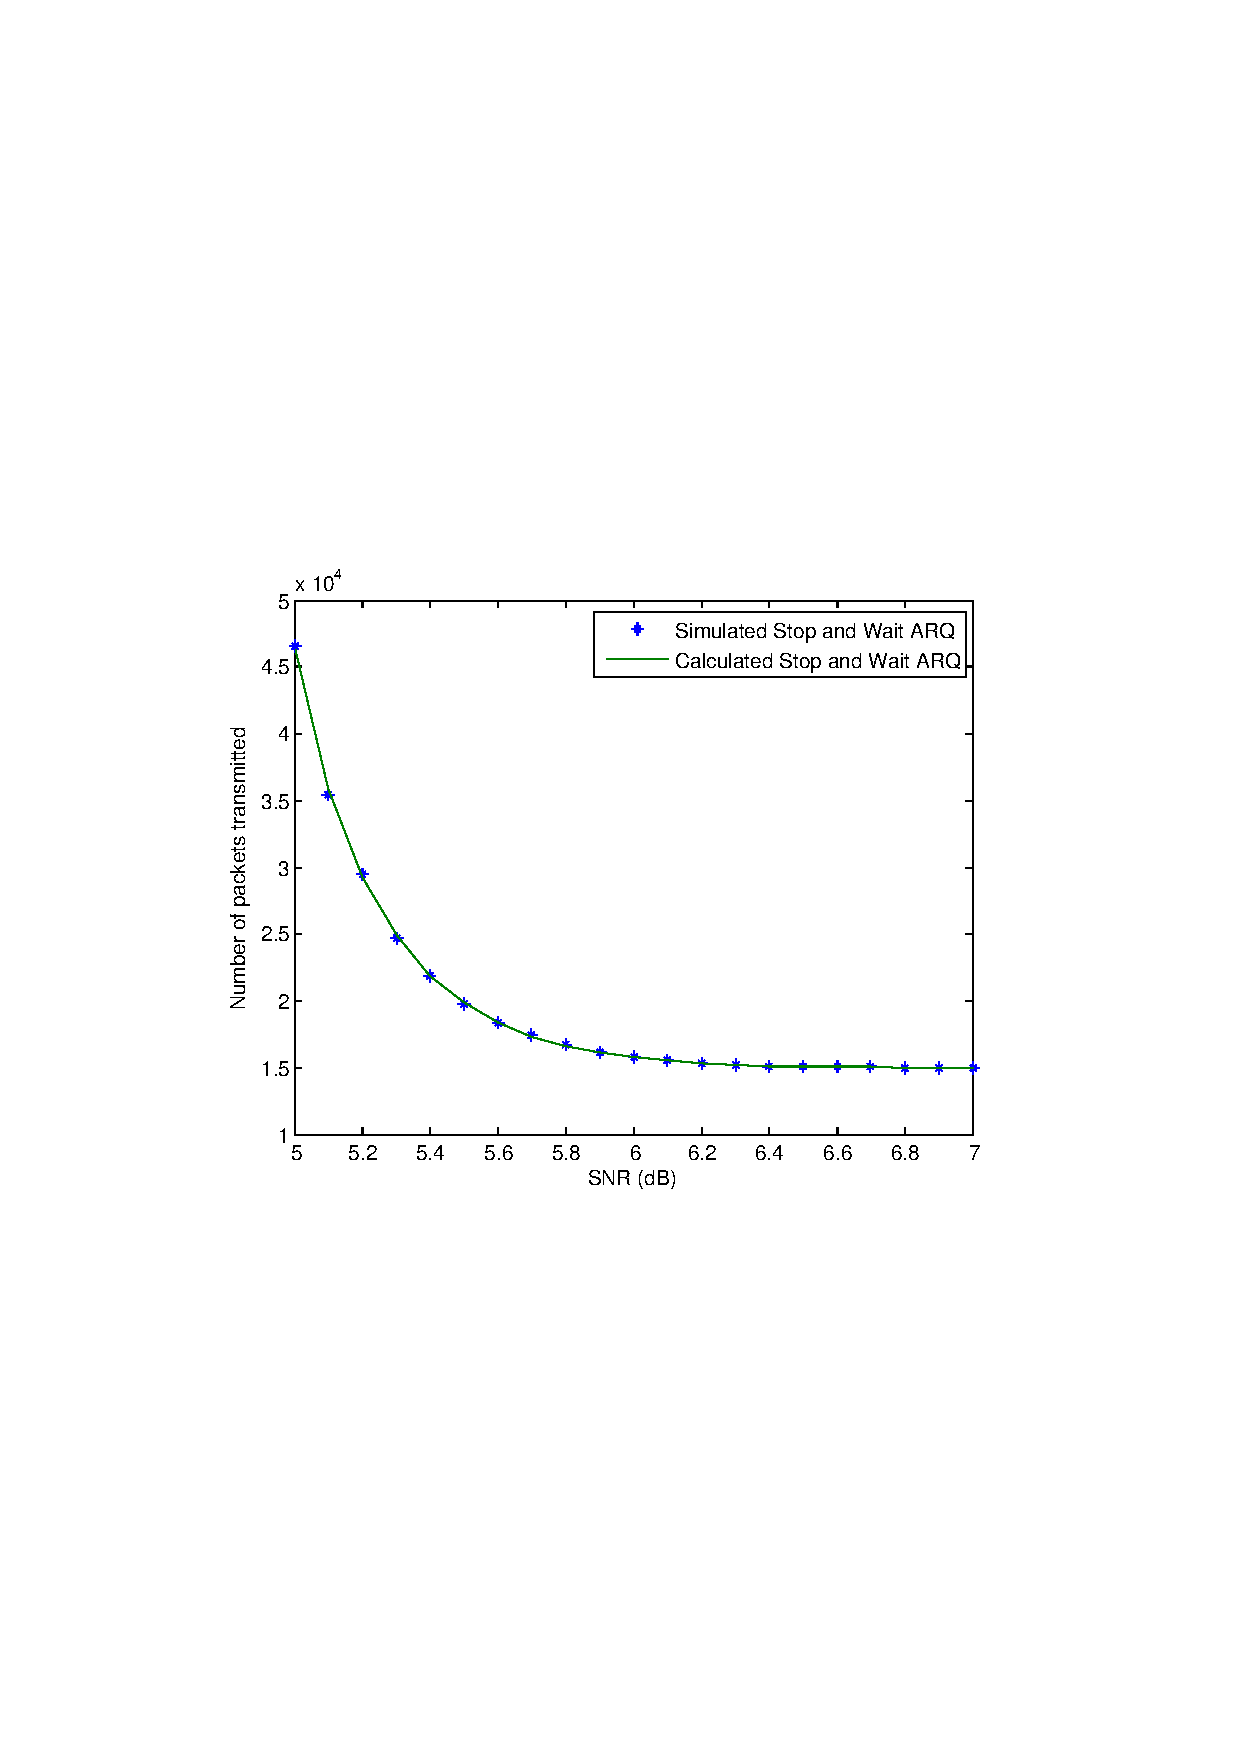
\includegraphics[width=140mm]{ComparisionSimulationVsCalculation.pdf}}
    \caption{Total number of packets transmitted to complete file transfer as a function of SNR. The simulated and theoretical results for Stop and Wait ARQ is shown for $N= 15000$ and $l=1440$.}
    \label{fig:ComparisionSimulationVsCalculation}
  \end{center}
\end{figure}

The simulation program counts the total number of packets transmitted to compete the file. For simplicity, a packet size of $l=1440$ bits is used. The simulation program is run 100 times, and the simulation results are averaged to reduce the mean squared estimation error. Figure~\ref{fig:ComparisionSimulationVsCalculation} illustrates total number of packets transmitted to complete file transfer using stop and wait ARQ, companying simulation to calculation. It shows that the simulation result closely matches the theoretical result, and the simulation method can be used in the following feedback analysis. From the figure, as SNR increases, the total number of packets transmitted decreases until approaching the lower bound, the file size 15000 packets.



\subsection{Transmission without Feedback}
\label{subsubNofeedback}
In the situation without feedback, linear transmission is used, that is, 15000 packets are transmitted from the beginning to the end periodically until 3 minutes pass. The transmission of 15000 packets from the beginning to the end is defined as one round.

Let $M_i$ be the round number when packet $i$ is successfully received, where $i=1, 2, 3 ...$. In rounds 1 to $M_i-1$, packet $i$ is in error. We assume $M_i$ is independent with $M_j$ for $i\neq j$.Then
\begin{align}
\Pr \left( {{M_i} \le m} \right) = 1 - {P_e}^m.
\end{align}

Let $M$ be the round number when all packets are finally successfully received. We have
\begin{align}
M=\mathop {\max }\limits_{i \in \left\{ {1,2,...,N} \right\}} \left\{ {{M_i}} \right\}.
\end{align}
The total number of packets transmitted to complete file transfer is on the interval $\left( {\left( {M - 1} \right)N,MN} \right]$. For simplicity, The upper bound $MN$ is used in comparison. Then for $ m=1,2,3...$
\begin{align}%{rcl}
%\begin{split}
\Pr \left( {M \le m} \right) &= \Pr \left( {\mathop {\max }\limits_{i \in \left\{ {1,2,...,N} \right\}} \left\{ {{M_i}} \right\} \le m} \right)&\\
 &= \Pr \left( {{M_1} \le m,{M_2} \le m,...,{M_N} \le m} \right)&\\
 &= {\left( {1 - {P_e}^m} \right)^N},&
\label{PMcdf}
\end{align}
and we can obtain the probability mass function
\begin{align}
\Pr \left( {M = m} \right) &= \Pr \left( {M \le m} \right) - \Pr \left( {M \le m - 1} \right)&\\
                           &= {\left( {1 - {P_e}^m} \right)^N} - {\left( {1 - {P_e}^{m - 1}} \right)^N},\quad m = 1,2,3....&
\end{align}
The expectation of $M$ is
\begin{align}
%\begin{split}
E\left[ M \right] &= \sum\limits_{m = 1}^\infty  {m\Pr \left( {M = m} \right)}&\\
\label{ExpectionM} \nonumber
&= \sum\limits_{m = 1}^\infty  {m\left[ {{{\left( {1 - {P_e}^m} \right)}^N} - {{\left( {1 - {P_e}^{m - 1}} \right)}^N}} \right]  }&\\
&= \sum\limits_{m = 1}^\infty  {m\left[ {\sum\limits_{k = 0}^N {{{\left( { - 1} \right)}^k} {N \choose k} } {P_e}^{mk} - \sum\limits_{k = 0}^N {{{\left( { - 1} \right)}^k}{N \choose k}} {P_e}^{\left( {m - 1} \right)k}} \right]}.&
%\end{split}
\end{align}
When $k=0$, ${\sum\limits_{k = 0}^N {{{\left( { - 1} \right)}^k}{N \choose k}} {P_e}^{mk} - \sum\limits_{k = 0}^N {{{\left( { - 1} \right)}^k}{N \choose k}} {P_e}^{\left( {m - 1} \right)k}}=0$. We have
\begin{align}
E\left[ M \right] &= \sum\limits_{k = 0}^N {{{\left( { - 1} \right)}^k}{N \choose k}} \sum\limits_{m = 1}^\infty  {m\left[ {{P_e}^{mk} - {P_e}^{\left( {m - 1} \right)k}} \right]}&\\ \nonumber
&= \sum\limits_{k = 1}^N {{{\left( { - 1} \right)}^k}{N \choose k}} \frac{{\left( {{P_e}^k - 1} \right)}}{{{P_e}^k}}\sum\limits_{m = 1}^\infty  {m{P_e}^{mk}}&\\ \nonumber
&= \sum\limits_{k = 1}^N {{{\left( { - 1} \right)}^k}{N \choose k}} \frac{{\left( {{P_e}^k - 1} \right)}}{{{P_e}^k}}\frac{{{P_e}^k}}{{{{\left( {1 - {P_e}^k} \right)}^2}}}&\\
&= \sum\limits_{k = 1}^N {{{\left( { - 1} \right)}^{k + 1}}{N \choose k}} \frac{1}{{1 - {P_e}^k}}.&
\label{ExpectationEMNoFeedback}
\end{align}

\begin{figure}[tpb]
  \begin{center}
    \centerline{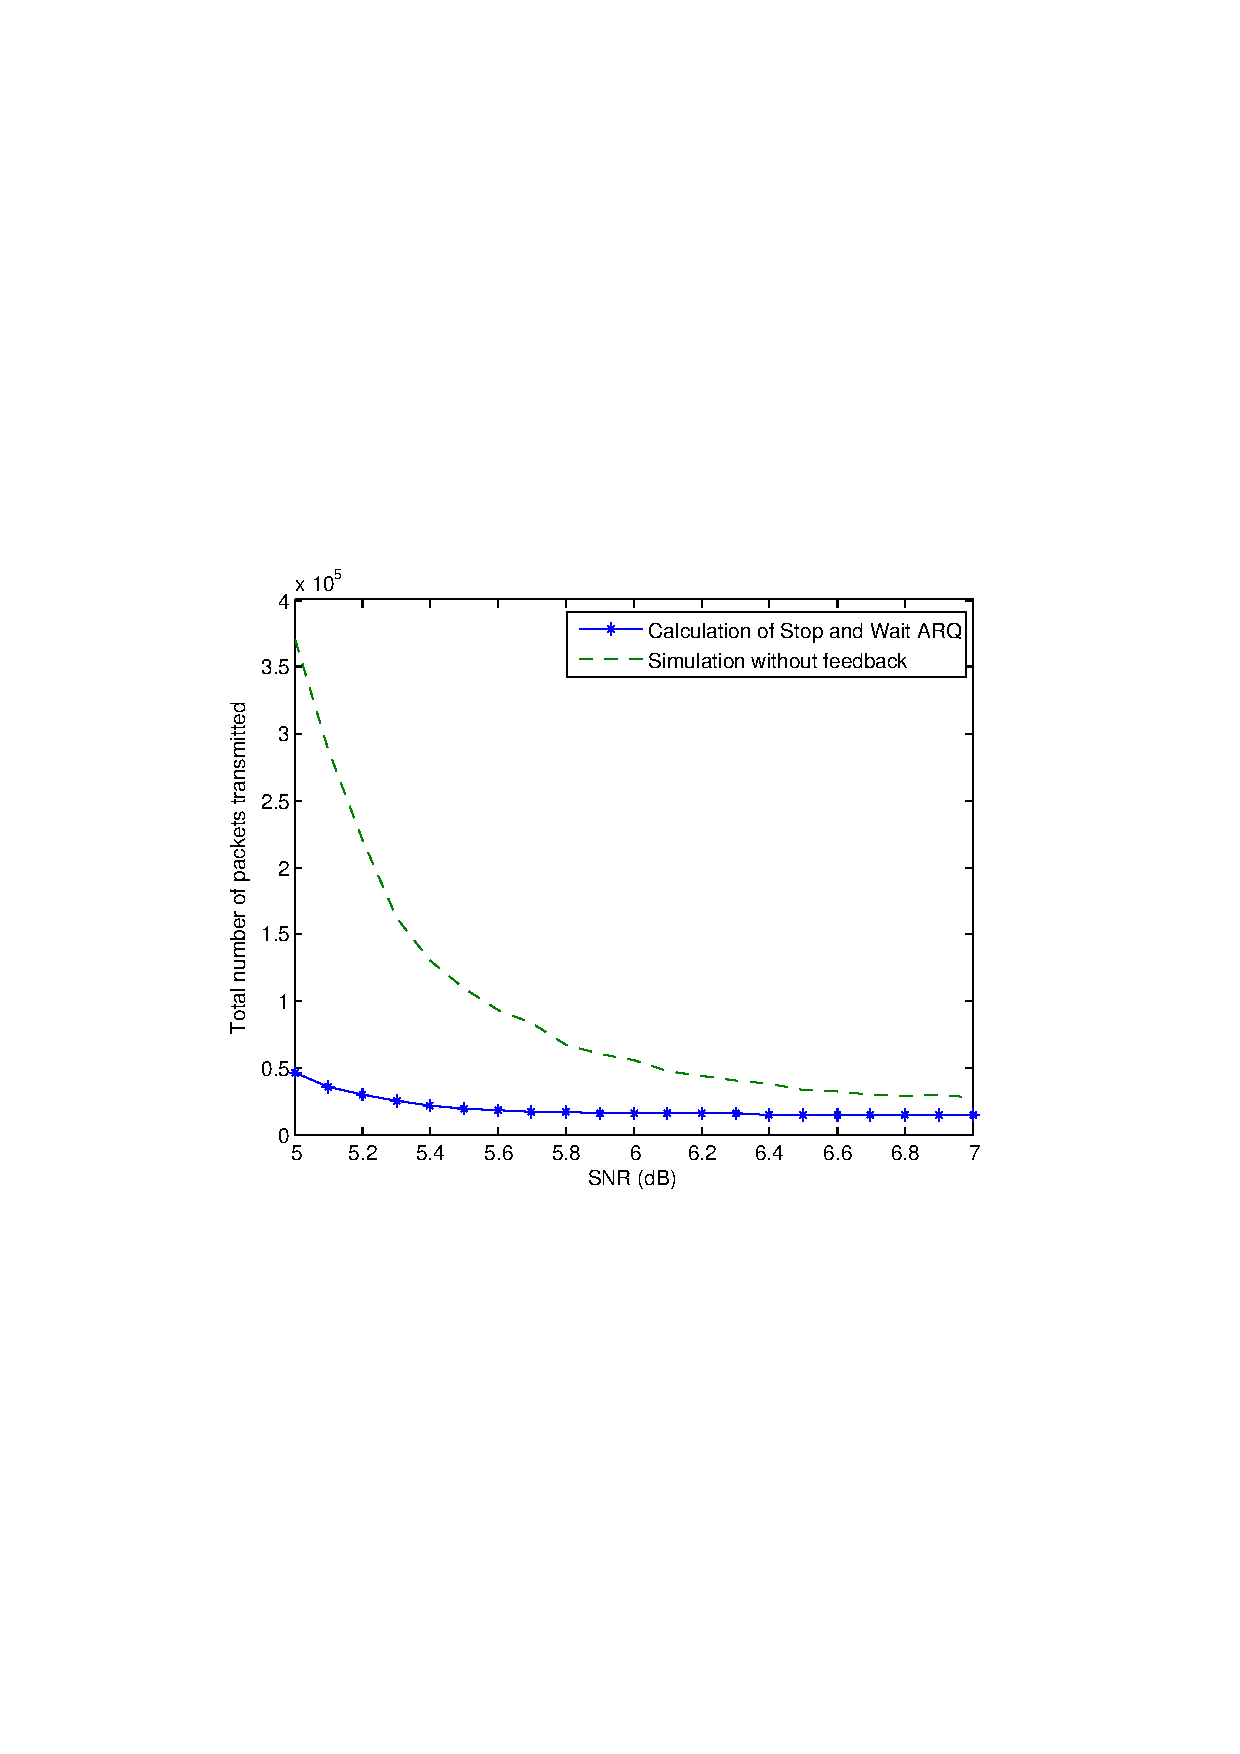
\includegraphics[width=140mm]{NoFeedbackSimulatoinandARQ.pdf}}
    \caption{Total number of packets transmitted to complete file transfer as a function of SNR for Stop and Wait ARQ  compared against that for Linear Transmission.}
    \label{fig:WithAndWithoutFeedback}
  \end{center}
\end{figure}

The precision of Matlab is not high enough to calculate $1 - {P_e}^k$, and a numeric value cannot be derived from (\ref{ExpectationEMNoFeedback}). Therefore simulation is primarily used to compare the performance of Stop and Wait ARQ and that  of Linear Transmission without feedback.

Figure~\ref{fig:WithAndWithoutFeedback} shows the simulation result with and without Stop and Wait ARQ. Without feedback, the total number of transmitted packets increases dramatically. As ${\rm{SNR}} \to \infty$, ${P_e} \to 0$, and from (\ref{ExpectionM}), we can conclude
\begin{align}
\mathop {\lim }\limits_{{\rm{SNR}} \to \infty } E\left[ M \right] = \mathop {\lim }\limits_{{\rm{SNR}} \to \infty } \sum\limits_{m = 1}^\infty  {m\left[ {{{\left( {1 - {P_e}^m} \right)}^N} - {{\left( {1 - {P_e}^{m - 1}} \right)}^N}} \right]}  = 1.
\end{align}
As a result, the total number of transmitted packets converges to 15000 as ${\rm{SNR}} \to \infty$.



\subsection{Highest Consecutive Packet Number Feedback}
In both the competitive and the cooperative matches, sending less feedback data allows for more time to be used in forward link data transmission. In Stop and Wait ARQ, every packet is acknowledged, which may require a significant amount of feedback data. Another feedback scheme, called Highest Consecutive Packet Number Feedback will be explored to reduce the amount of feedback data. In Highest Consecutive Packet Number Feedback, only one number is sent in the feedback data to indicate that all packets with packet number less than or equal to the number have been successfully received. Once the source receives the highest consecutive packet number, the next round of transmission starts with the highest consecutive packet number plus one.

\begin{figure}[tpb]
  \begin{center}
    \centerline{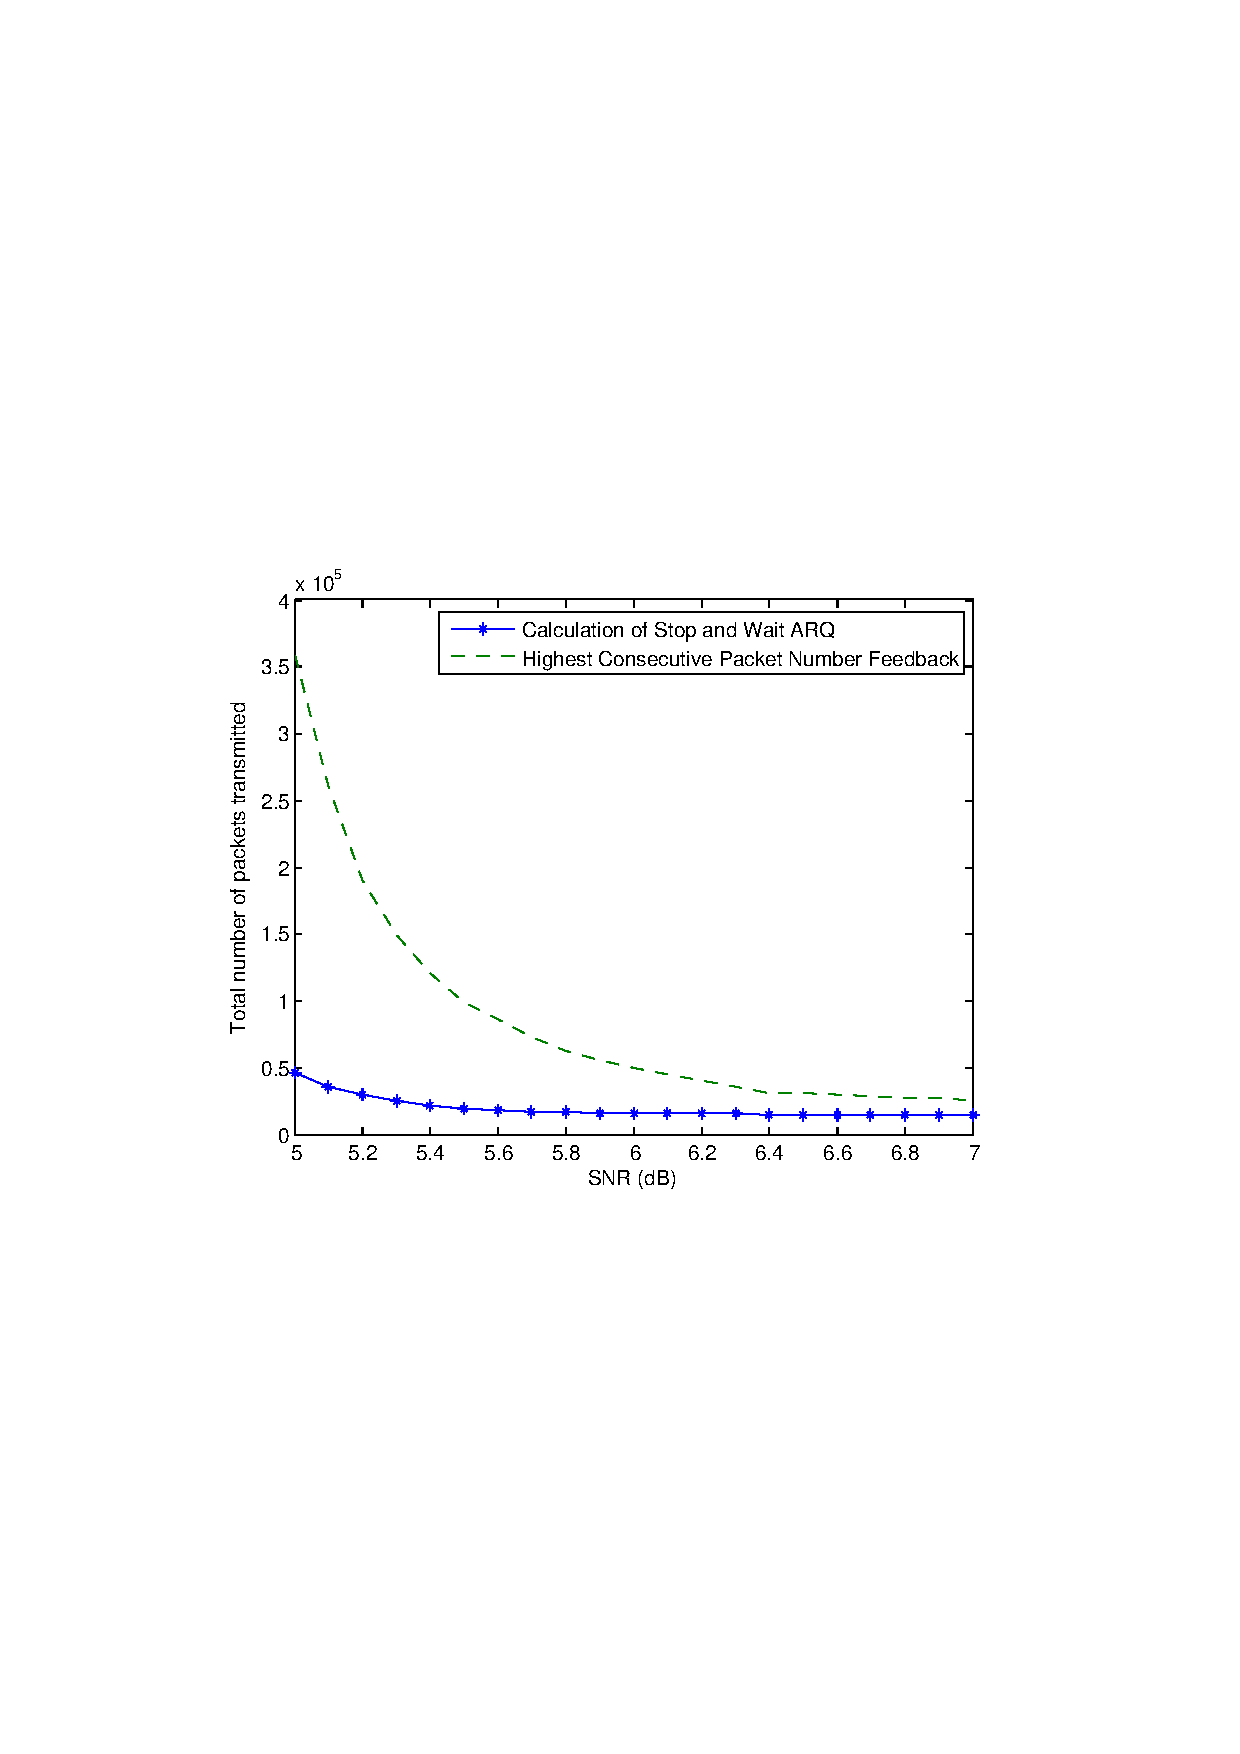
\includegraphics[width=140mm]{HighestPktNoFeedbackSimulatoinandARQ.pdf}}
    \caption{Total number of packets transmitted to complete file transfer for Stop and Wait ARQ compared against that for Highest Consecutive Packet Number Feedback.}
    \label{fig:HighestPktNoFeedbackSimulatoinandARQ}
  \end{center}
\end{figure}

Figure~\ref{fig:HighestPktNoFeedbackSimulatoinandARQ} illustrates the total number of packets transmitted to complete file transfer for Stop and Wait ARQ  and for Highest Consecutive Packet Number Feedback. The total number of transmit packets is much higher than that of Stop and Wait ARQ. By compare Figure~\ref{fig:WithAndWithoutFeedback} with Figure~\ref{fig:HighestPktNoFeedbackSimulatoinandARQ}, we see that the total number of packets transmitted is only slightly lower in Highest Consecutive Packet Number Feedback than in Linear Transmission.

Highest Consecutive Packet Number Feedback greatly reduces the amount of feedback data, but has low efficiency.


\subsection{Group Feedback}
Stop and Wait ARQ and Highest Consecutive Packet Number Feedback are two extreme situations in terms of performance and cost. Another type of feedback, Group Feedback, is explored to balance the performance and cost. In Group Feedback, one feedback number acknowledges that a group of packets with a given consecutive packet number has been received. The default method is to transmit all the unacknowledged file packets from the lowest to the highest packet number round by round. Let the group size be $S$. A group feedback number $k$ means packets with packet number $(S-1)k+1$ to $Sk$ have been received.

For example, if $S=5$ and the source receives a feedback number $k=1$, it means the receiver has successfully received packets with number 1 to 5. If $S=1$, Group Feedback is equivalent to Stop and Wait ARQ. Within each group, say Group $i$, it is equivalent to transmission without feedback with $N=S$ as discussed in Section \ref{subsubNofeedback}. If $S=15000$, the total packet number in the file, Group Feedback is equivalent to transmission without feedback. From (\ref{ExpectationEMNoFeedback}), the expected total number of packets transmitted to complete file transfer
\begin{align}
E\left[ {{n_t}} \right] = N\sum\limits_{k = 1}^S {{{\left( { - 1} \right)}^{k + 1}}{S \choose k}} \frac{1}{{1 - {P_e}^k}},
\end{align}
which is not good for numeric calculation in Matlab because the precision of Matlab is not high enough as the discussed in Section \ref{subsubNofeedback}. We again use simulation to compare performance.

Another concept, called feedback compression rate (denoted $R_f$) is used. Suppose, one feedback packet can represent $n_f$ data packets when $S=1$. Feedback compression rate can be defined as
\begin{align}
{{\rm{R}}_f} = \frac{{{n_f}}}{S}.
\end{align}
Typical value of $n_f$ ranges from 1/30 to 1/12 in our radios. Consider a worse situation, and $n_f=0.2$ is used. Suppose the number of packets in the data link to be $n_d$. The total number of packets in both the data link and the feedback link can be expressed as
\begin{align}
{n_t} = {n_d}\left( {1 + {{\rm{R}}_f}} \right) = {n_d}\left( {1 + \frac{{{n_f}}}{S}} \right).
\end{align}

Figure~\ref{fig:GroupFeedback} illustrates the simulation result of group feedback. In low SNR, such as 5 dB, the total number of total transmitted packets in both links increases dramatically, as the group size $S$ increases. It shows $S=1$ is better in low SNR. In relatively high SNR, such as 7 dB, group feedback with $S>1$ is slightly better than that with $S=1$. In both the competitive and cooperative matches, harsh environments with low SNR, should be considered. Therefore, $S=1$, namely Stop and Wait ARQ, is preferred.

\begin{figure}[tpb]
  \begin{center}
    \centerline{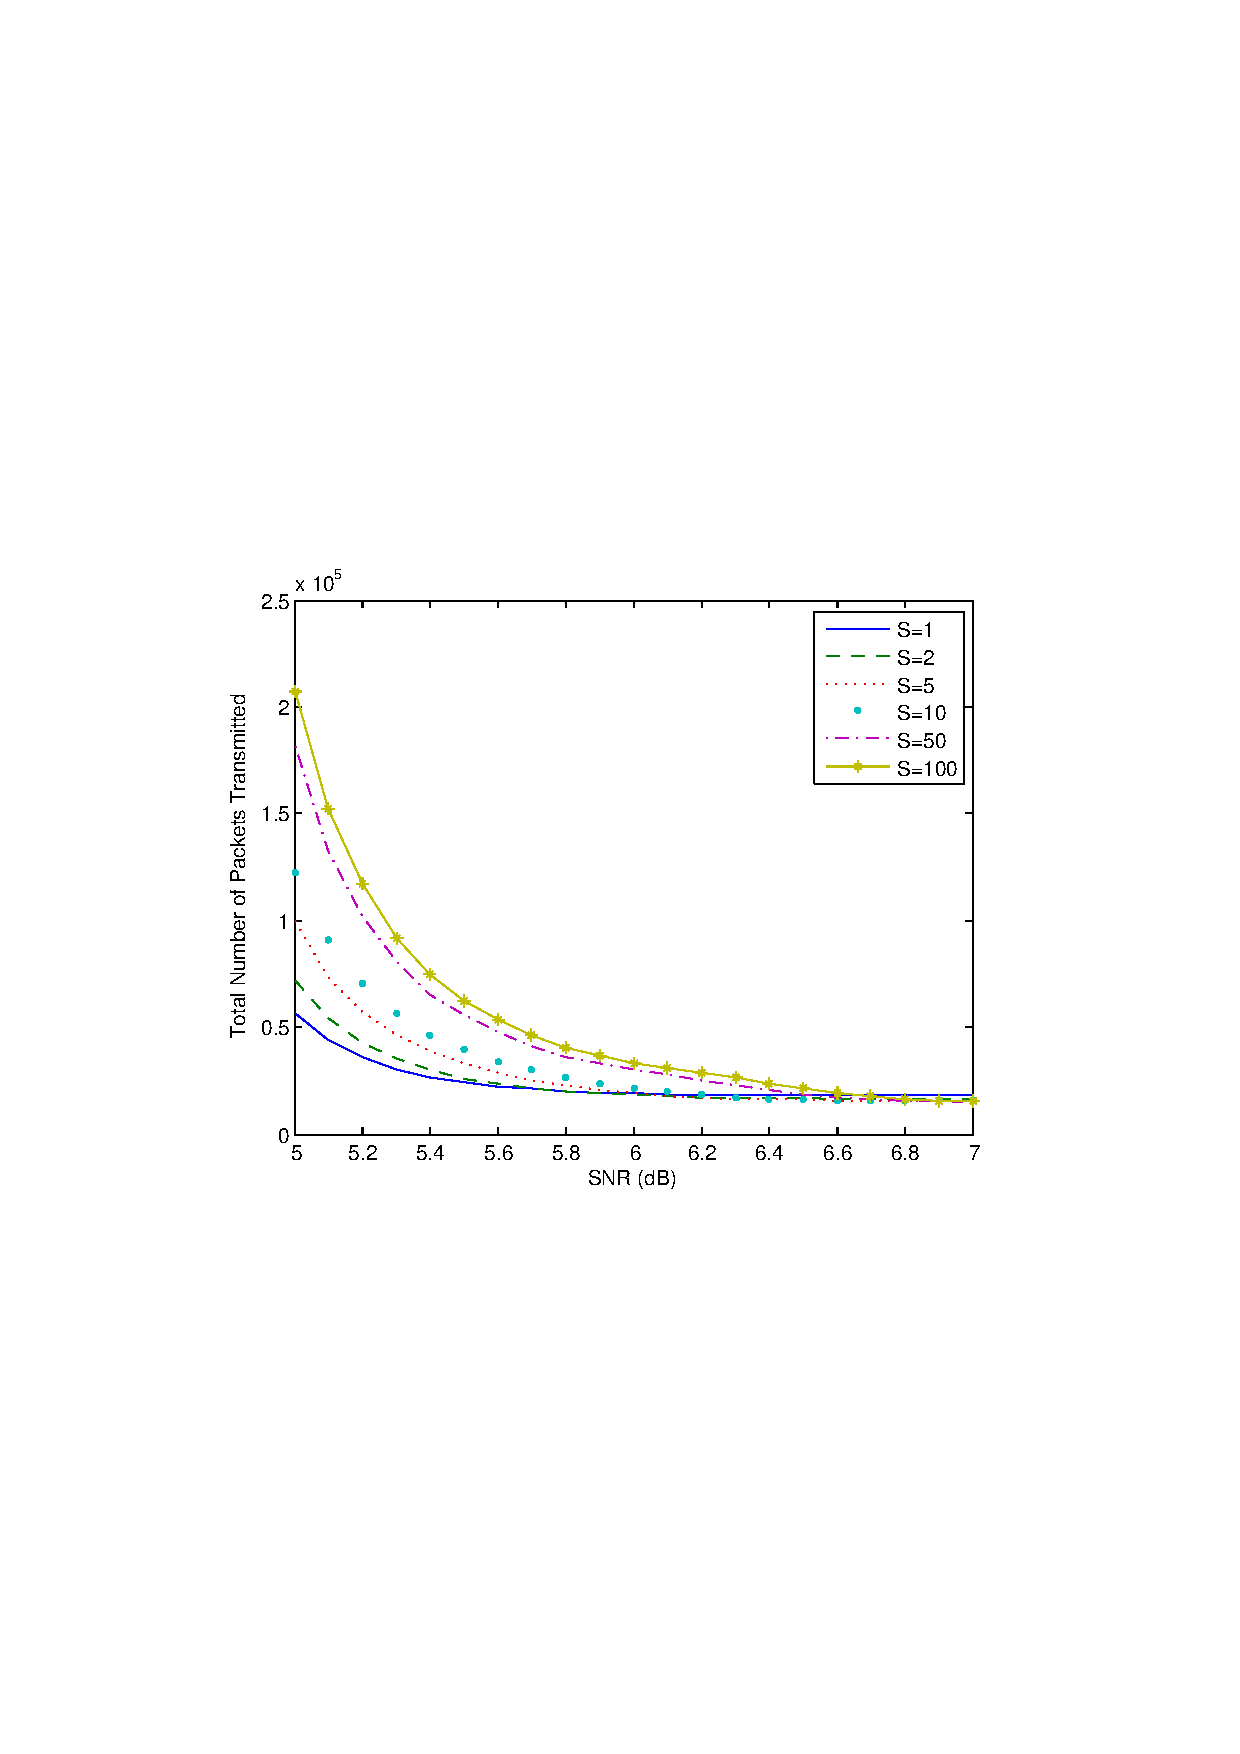
\includegraphics[width=140mm]{GroupFeedback.pdf}}
    \caption{Total number of packets transmitted in both data link and feedback link to complete file transfer for Group Feedback. $n_f=0.2$.}
    \label{fig:GroupFeedback}
  \end{center}
\end{figure}

It seems that group feedback is useless in our radio, but a modified version of group feedback can be used to significantly improve the feedback performance when practical situations are considered, which will be discussed in Section \ref{feedbackDesign}.

\subsection{Sliding Window ARQ}
In the Stop and Wait ARQ discussed in Section \ref{subsubStopAndWaitARQ}, the feedback delay, including data transmission time, receiver data processing time and ACK time, is assumed to be 0, but the assumption does not apply in practice. Sliding Window ARQ is used to solve the problem of feedback delay in the manner described below.

In Sliding Window ARQ, the source maintains a window of source packets. Suppose the size of the window is $S_w$, which corresponds to shift registers of size $S_w$ containing the packets to be transmitted. The registers are assigned a serial number as $\left( {{\rm{1, 2, }}...{\rm{, }}{{\rm{S}}_w}} \right)$. The source transmits the packet in the first register and then the second packet even if it has not received an ACK of the first packet from the destination. If the source transmits all the $S_w$ packets in the transmitting window, it will repeat the process by transmitting the packet in the first register and so on. Once the source obtains an ACK of any packet in the shift registers, the shift registers shift to flush that packet and get a new packet and put it in register $S_w$.

The key parameter in Sliding Window ARQ is the window size $S_w$. The window size should be large enough to ensure that the time of one transmission round of data in the window is larger than the feedback delay. If the window size condition is satisfied, the performance of Sliding Window ARQ is equal to that of Stop and Wait ARQ.


\section{Feedback Design}
\label{feedbackDesign}
Based on the analysis in Section \ref{secAnalysisFeedback}, Sliding Window ARQ will be used in our radio. However, the analysis of feedback is based on the assumption that the reverse link (feedback link) is reliable. Actually, in both competitive and cooperative match, the reverse link cannot guarantee 100 $\%$ reliable transmission, even with channel coding, because of the unpredictable interference from the competitor and cooperators. There is a certain non-zero probability that acknowledgements from the receiver may be lost or corrupted.

To compensate for the unreliability of the reverse link, the destination keeps sending acknowledgements of all the received packets round by round. However, another problem arises. If every single packet is acknowledged by a feedback number, the total feedback data would increase dramatically as the number of successfully received packet increases. We will use a complex feedback that combines the Sliding Window ARQ, Highest Consecutive Packet Number Feedback, and Group Feedback. For this complex feedback,  there is a number indicating the highest consecutive packet number in every feedback packet, and the rest of the acknowledgements are represented by Group Feedback with multiple group size. The values $S =5$, $S=20$, $S=100$ and $S=500$ are used for cooperative radio and $S =5$, $S=30$ and $S=200$ are used for competitive radio. If all packets in a larger group have been received, a single feedback number will be sent to acknowledge all packets in the group have been received. Otherwise, a smaller group will be used and so on.

\subsection{Bit level design for cooperative radio}

In cooperative radio, each physical-layer packet has 116 bytes to carry data and 4 bytes for CRC check. Five bytes are used for a header, and 111 bytes are used to carry a sub-packet. As a result, each application packet of size 1440 bytes from the server is divided into 13 sub-packets. The first 12 sub-packets have 111 bytes and the last one has 108 bytes. In the header, two bytes are used for indicating the packet number and one byte is used for the sub-packet number. The left two bytes in the header are reserved.

In the feedback link, a physical-layer packet also has 116 bytes of data. One byte is used to indicate whether all the packets have been successfully received, and two bytes are used for Highest Consecutive Packet Number Feedback. For all the remaining bytes, 4 bytes are used as a group. The first two bytes indicate the packet number and 13 bits of the other two bytes are used as bitmap to show whether each individual sub-packet has been received. If group feedback is used, hexadecimal numbers 3FFF, 7FFF, BFFF and FFFF are set in the two-byte bitmap to stand for group feedback with group size $S =5$, $S=20$, $S=100$, and $S=500$ respectively.


\subsection{Bit level design for competitive radio}
In competitive radio, uncoded QPSK with rate 1, QPSK with rate 1/2 repetition code, BPSK with 1/2 repetition code and BPSK with 1/4 repetition code lead to MAC payload sizes of 236 bytes, 116 bytes, 56 bytes and 26 bytes respectively. To meet the requirement of variable MAC payload size, a sub-packet size of 23 bytes is used. Three bytes are added to the sub-packet to indicate the packet number and sub-packet number. Therefore each sub-packet needs 26 bytes in total.  Each 1440-byte application packet is divided into 63 sub-packets.  The first 62 sub-packets each has 23 bytes, and the last one has 14 bytes. Each MAC payload tries to fill as many sub-packets as possible.

In the feedback, QPSK with rate 1/2 repetition code is used and each MAC payload has 116 bytes. As in the cooperative radio, one byte is used to indicate whether all the packets have been successfully received, and two bytes are used for Highest Consecutive Packet Number Feedback. If not all the sub-packets in a packet are received, the feedback data has 10 bytes. Two of bytes are used for the packet number, and the other 8 bytes form a 64-bit bitmap to indicate whether each sub-packet is received. If group feedback is used, only two bytes are used for feedback. The 14 least significant bits of the two bytes are used for the packet number and the most significant two bits are used to indicate group feedback. If the two bits are 00, there will be another eight bytes for sub-packet bitmap feedback. The bits patterns 01, 10 and 11 stand for group feedback with group size $S =5$, $S=30$ and $S=200$ respectively. The Two-byte hexadecimal number FFFF is used to indicate the end of feedback data in a MAC payload.





%
% Chapter 5
%

\chapter{SPECTRUM ANALYSIS}
\label{chap:spectrumAnalysis}

Spectrum analysis is a key component of our cooperative strategy. This chapter will discuss the spectrum sensing techniques. Based on the characteristics of the USRP, a new spectrum sensing algorithm is proposed.

\section{Spectrum Sensing}
\label{SpectrumSensingIntro}
The three major types of spectrum sensing techniques include matched filter detection, feature detection, and energy detection \cite{HanoWangGosanNohDongkyuKimSungtaeKimandDaesikHong2010}. In this section, only one frequency band is taken into consideration.

\subsection{Matched Filter Detection}
In digital communication, the matched filter is often used by the receiver to demodulate the digital information from the received waveform \cite{JGProakisMasoudSalehi}. If the primary user's signal is known to the secondary user, the matched filter can also be used to detect whether the primary user is using the spectrum. It is widely known that detection using a matched filter can achieve the optimum performance in white Gaussian noise when a secondary sensing node can perform a coherent detection of the primary user's signal \cite{DCabricandSMMishraandRWBrodersen2004}. With matched filter based sensing, it takes less time to achieve a limited probability of a missed detection and a false alarm. The required number of samples is inversely proportional to the SNR for a given confidence level of a false alarm \cite{R.TandraandA.Sahai:2005}. The main defect for matched filter detection is that the sensing node must have prior knowledge of other radios such as the preamble signaling for synchronization, modulation scheme, etc., which may not be possible.

\subsection{Feature Detection}
The feature detection method utilizes some features of the radios using this spectrum band. Since no prior knowledge is known in the Spectrum Challenge, this technique cannot be used, but we still briefly introduce it.

\subsubsection{Waveform Based Sensing}
In waveform based sensing, the sensing node needs to know the patterns of the other radios, such as preambles, pilots, and spreading sequences. Sensing can be performed by correlating the received signal with known signals \cite{A.SahaiandR.TandraandS.M.MishraandN.Hoven:2006}. The difference between matched filter detection and waveform based sensing is that matched filter detection requires perfect modulation information of primary users while the waveform based sensing only needs some signal patterns of the primary users.

\subsubsection{Cyclostationarity-Based Sensing}
Cyclostationary features can be used for spectrum sensing. Usually cyclostationary features are inherent in the signal's statistics, such as mean and autocorrelation, or through the signal's periodicity. In addition, cyclostationary can be introduced into the primary users' signal to aid spectrum detection. Some OFDM systems have been altered to adapt to the requirements of cyclostationarity-based sensing \cite{P.D.SuttonandK.E.NolanandL.E.Doyle:2007}. Since noise is often modeled as wide-sense stationary (WSS), cyclostationarity-based detection can more easily distinguish between the users' signal and noise.

\subsubsection{Radio Identification Based Sensing}
Knowledge about the spectrum characteristics can be obtained by learning the transmission technologies of transmitting users, and such characteristics can be used to help characterize spectrum usage. For instance, suppose one radio can be identified as employing WiFi signals. The sensing node can use this information to conclude that the radio should be within 100 meters. In radio identification based sensing, several features can be used to determine the transmission technologies. These features include amount of the energy detected and the energy distribution across the spectrum, channel bandwidth and the shape signal \cite{J.PalicotandC.Roland:2003}. These features are fed to a Bayesian classifier for determining the active radios.

\subsection{Energy Detection}
Energy detection is the most common spectrum sensing technique. It has low implementation and computational complexities \cite{M.Wylie-Green:2005}. Receivers that use energy detection do not need detailed knowledge of the modulation schemes of the primary users. They only need to detect whether the signal level exceeds a certain threshold determined by the noise level. Assume $s(n)$ is the primary uses' signal, $w(n)$ is additive white Gaussian noise (AWGN) and $y(n)$ is the received signal of the secondary user. The system model is
\begin{align}
y(n)=s(n)+w(n).
\label{systemModel}
\end{align}
Making a decision whether primary users are using the spectrum is equivalent to the following hypotheses:
\begin{align}
&\mathcal{H}_0:y(n)=w(n)\\
&\mathcal{H}_1:y(n)=s(n)+w(n).
\end{align}
Here $\mathcal{H}_0$ is the null hypothesis that the primary users are not using the spectrum, while $\mathcal{H}_1$ is the hypothesis that the primary users are using the spectrum.

The decision statistic based upon received energy is
\begin{align}
E=\frac{1}{N}{\sum\limits_{n = 1}^N {\left| {y(n)} \right|} ^2}.
\label{decisionMetricTime}
\end{align}
Define the probability of detection to be $P_D$, the probability of false alarm to be $P_F$, and the probability of missed detection to be $P_M$. Then
\begin{align}
&P_D=P_r(E > \lambda_E | \mathcal{H}_1)
\label{Detectionprobability}\\
&P_F=P_r(E > \lambda_E | \mathcal{H}_0)\\
&P_M=P_r(E \leq \lambda_E | \mathcal{H}_1)=1-P_D,
\end{align}
where $\lambda_E$ is the detection threshold of energy detection.  The threshold $\lambda_E$ should be selected such that both $P_F$ and $P_M$ are as small as possible. However, a tradeoff exists between $P_F$ and $P_M$.  The threshold $\lambda_E$ depends on the noise variance, and even a small estimation error of noise variance would cause a significance detection error \cite{A.SahaiandN.HovenandR.Tandra:2004}. To solve this problem, the noise level can be estimated by separating the signal subspaces and noise dynamically with the multiple signal classification (MUSIC) algorithm \cite{M.P.OlivieriandG.BarnettandA.LackpourandA.Davis:2005}.

\section{Design and Implementation of a Spectrum Analyzer}
From the discussion of Section \ref{SpectrumSensingIntro}, only energy detection does not requires prior knowledge of the characteristics of other radios. As a result, energy detection will be used in our spectrum analyzer.

From Chapter \ref{chap:strategy}, our cooperative radio tries to occupy the entire spectrum left by others. To fulfill this requirement, the 5 MHz bandwidth is divided into 16 sub-bands, and each sub-band can be setup to be used or not based upon energy detection in each sub-band. The data transmitted by each sub-band should not depend on the success of other sub-bands. Define the data transmitted by each sub-band as a physical-layer packet. This process can be viewed as quantization of frequency. Even if only part of the sub-band is used by other radios, it should be marked as used. Therefore, decreasing the bandwidth of each sub-band gives us more spectrum opportunities. In practice, a physical-layer packet should have header information to tell what is included. The length in time of each sub-band has been fixed by the physical layer. If the bandwidth of a sub-band is too small, most of the information carried by a physical-layer packet is header information. Only a small amount of data is transmitted, and the total efficiency decreases. As discussed in Chapter \ref{chap:backgound}, the number of sub-bands for both data transmission is 16, and the number of sub-band for spectrum sensing is also selected to be 16 such that the tone assignment for each sub-band is the same for both data transmission and spectrum sensing.


Figure \ref{fig:SpectrumAnalyzerFlowChart} shows the flow chart of the spectrum analyzer. The software component of the analyzer consists of preprocessing and decision making.

\begin{figure}[tpb]
  \begin{center}
    \centerline{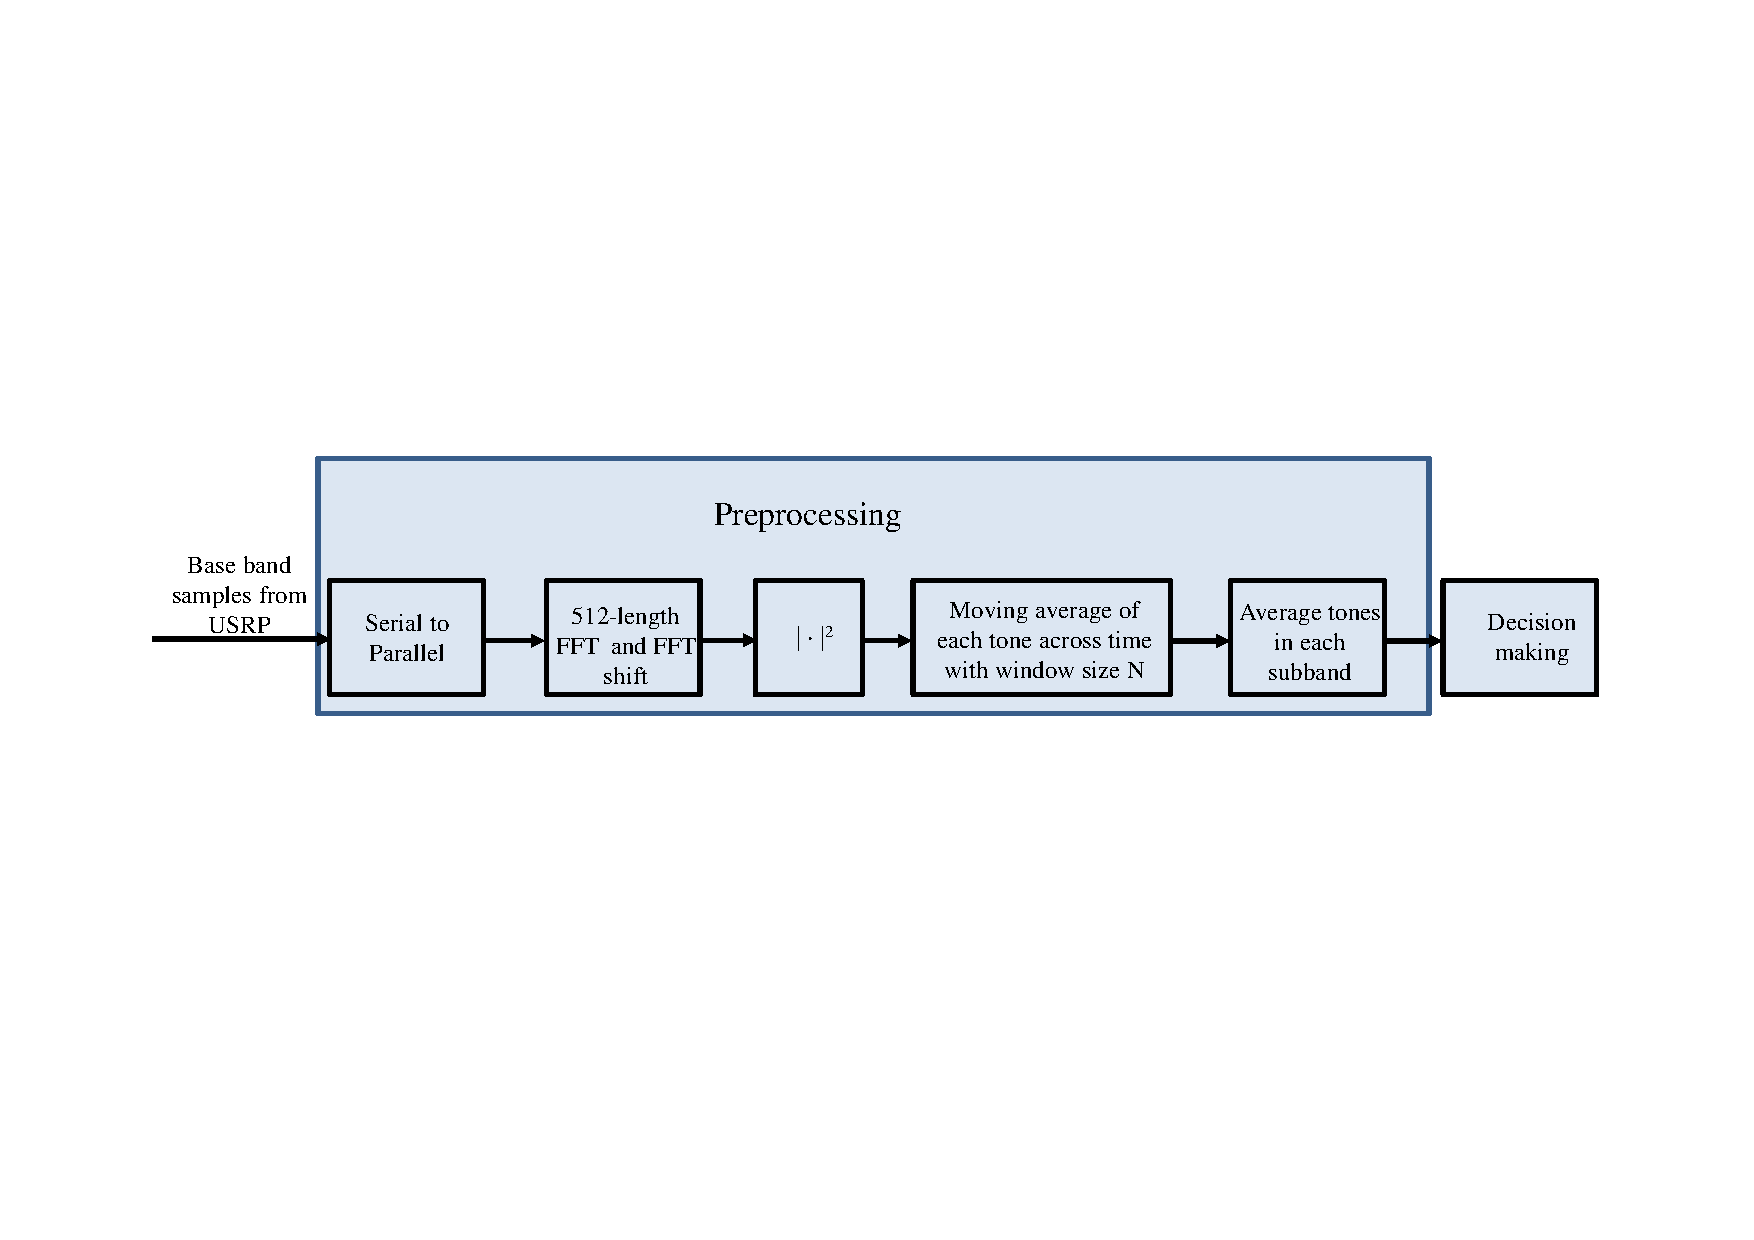
\includegraphics[width=160mm]{SpectrumAnalyzerFlowChart.pdf}}
    \caption{Flow Chart of Spectrum Analyzer}
    \label{fig:SpectrumAnalyzerFlowChart}
  \end{center}
\end{figure}

\subsection{Preprocessing}
First, the serial samples from the USRP are converted to parallel signal with length 512. Second, a length 512 FFT is conducted to convert the signal from the time-domain to the frequency-domain. An FFT shift is conducted to convert the signal from $\left[ {0,2\pi } \right)$ to $\left[ { - \pi ,\pi } \right)$ such that the DC tone is in the center and has index 257. Third, the energy of each frequency sample is calculated. Fourth, the moving average of each tone across time is computed as
\begin{align}
{E_j} = \frac{1}{N}\sum\limits_{n = 1}^N {{{\left| {{s_j}(n)} \right|}^2}}, \quad j = 1,2,...,512,
\label{decisionMetricfreq}
\end{align}
where ${s_j}(n)$ is the signal of tone $j$ at time $n$. Equation (\ref{decisionMetricfreq}) is a modified version of (\ref{decisionMetricTime}). Fifth, the tones in each sub-band are averaged according to
\begin{align}
{E_i} = \frac{1}{M}\sum\limits_{j \in {\rm{sub\mbox{-}band}} \ i}^{} {{E_j}} , \quad i = 1,2,...,16,
\label{subbandEnergy}
\end{align}
where $M$ is the number of tones in each sub-band. Here we have $M=30$.

The feedback of the cooperative radio is sent with a 200 kHz OFDM signal, and the center frequency of the feedback is in the middle of the sub-band that has lowest average energy. In other words, the feedback band is within sub-band ${i^*} = \mathop {\arg \min }\limits_{{\rm{i  =  1,2,}}...{\rm{,16}}} \left\{ {{E_i}} \right\}$.


\subsection{Decisions Making}
In energy detection, comparing the energy of a sub-band to a threshold is the way to decide if the sub-band is used by other radios. However, we observed that sometimes the energy detection used in (\ref{Detectionprobability}) is too conservative. For example, there are strong side lobes for the signal generated by the GNU Radio and the USRP as illustrated in Figure \ref{fig:SginalWithSideLobe}, which was generated by a hardware spectrum analyzer. There are three energy levels in the signal. The highest energy level is the information signal that carries data from the cooperator. The second highest energy level is the side lobe of the cooperator's signal. The lowest energy level is the noise floor. The spectrum occupied by the side lobes can still be used to transmit data as long as we are not generating interference for our cooperators.
\begin{figure}[tpb]
  \begin{center}
    \centerline{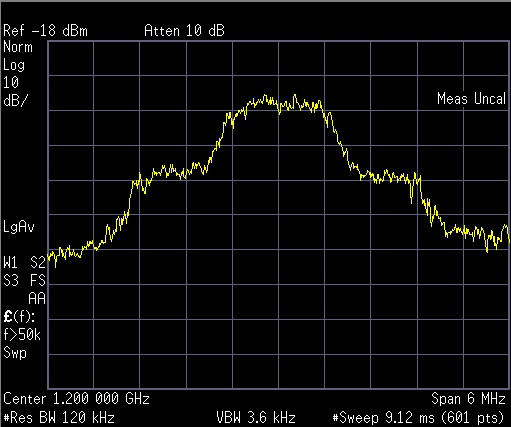
\includegraphics[width=140mm]{SginalWithSideLobe.jpg}}
    \caption{Example of a signal with large side lobes}
    \label{fig:SginalWithSideLobe}
  \end{center}
\end{figure}

A new algorithm is proposed to address the conservative nature of energy detection in the case of strong side lobes. The assumption of the algorithm is that the side lobes are much smaller than main lobe. If the energy level of the side lobes is equivalent to that of the information signal, we cannot distinguish them.

\subsubsection{Signal Model}
As shown in Figure \ref{fig:SpectrumAnalyzerModel}, there are a total of $K=16$ sub-bands, and sub-band $i$ has energy $E_i$ as described in (\ref{subbandEnergy}).We classify signals as the information signal, the side lobe, and the noise. Suppose the information signal energy has mean $m_1$ , and the side lobe energy has mean $m_2$.
\begin{figure}[tpb]
  \begin{center}
    \centerline{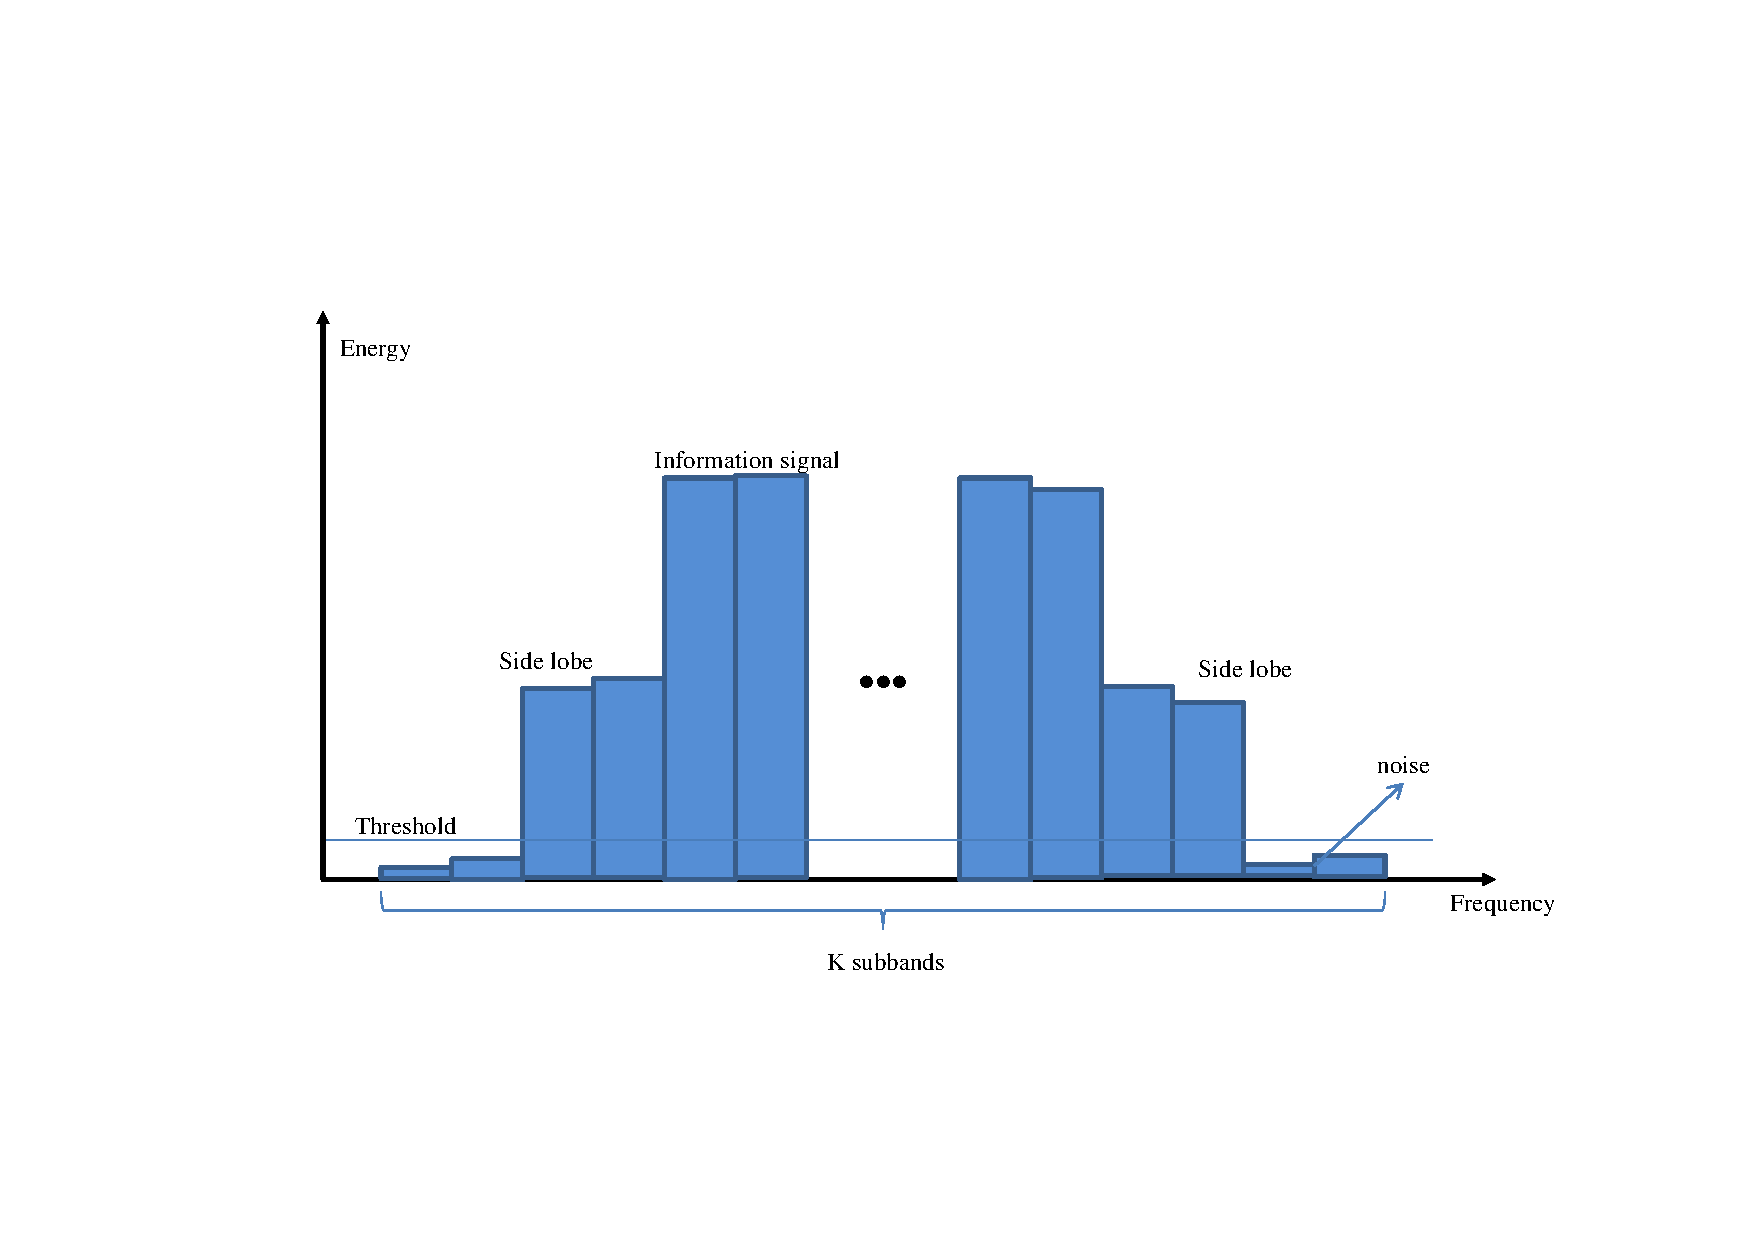
\includegraphics[width=140mm]{SpectrumAnalyzerModel.pdf}}
    \caption{Model illustration of spectrum analyzer}
    \label{fig:SpectrumAnalyzerModel}
  \end{center}
\end{figure}
\subsubsection{Decision Procedures}
First, compare $E_i$ with a threshold $\lambda>0$. If
\begin{align}
E_i < \lambda,
\end{align}
sub-band $i$ is available for use.

Second, consider all the sub-bands for which $E_i  \ge \lambda$. Define
\begin{align}
\mathcal{R}_0 =\left\{ {i:{E_i} \ge \lambda } \right\}.
\end{align}
Suppose the sample mean of their energy is $m_0$ and the sample variance deviation is $S_0^2$, where
\begin{align}
{m_0} = \frac{1}{{\left| \mathcal{R}_0 \right|}}\sum\limits_{i \in \mathcal{R}_0} {{E_i}}
\end{align}
\begin{align}
S_0^2 = \frac{1}{{\left| \mathcal{R}_0 \right| - 1}}\sum\limits_{i \in \mathcal{R}_0} {{{\left( {{E_i} - {m_0}} \right)}^2}}.
\end{align}

If the number of sub-bands in $\mathcal{R}_0 $ is less than 4, we terminate; treating all the remaining sub-bands as a cooperator's signal. The reason for this procedure is that the variance is difficult to estimate from a small sample. Otherwise, if
\begin{align}
\gamma S_0<m_0,
\label{smallvariance}
\end{align}
we treat all the remaining sub-bands as signal from the cooperator and terminate. Here, $\gamma$ is a coefficient to be determined. The reasoning behind (\ref{smallvariance}) is that a small value of $S_0$ indicates that there is not a side lobe, or the side lobes have a similar energy level to the information signal, which cannot be distinguished using energy detection. This step also avoids the situation in which the entire 5 MHz spectrum is occupied by a uniformly distributed signal across frequency.

Finally, for all sub-bands with $E_i \ge \lambda$, if
\begin{align}
E_i \le m_0-\beta S_0,
\label{DecisionCretia}
\end{align}
then sub-band $i$ is available to use, because sub-band $i$ is occupied by a side lobe. Otherwise, sub-band $i$ is considered to be part of the cooperator's information signal.

\subsubsection{Determination of Coefficients $\gamma$ and $\beta$}
The parameter $\gamma$ is used to decide whether there is side lobe. It should be a real number larger than 1, and it is determined by the variance of the cooperator's signal. Two USRPs are used to measure the sample mean to standard deviation ratio. One is used as the spectrum analyzer and the other is used as the interference source. The distance between the two USRPs is about 3 feet. A single-band signal with low-energy side lobes as shown in Figure \ref{fig:SAsingleNoSideLobe} and a single-band signal with large bandwidth as shown in Figure \ref{fig:SASingleLargeBand}, are tested to determine $\gamma$. Twenty tests are conducted. For the information signal, the sample mean to standard deviation ratio in Figure \ref{fig:SAsingleNoSideLobe} is 2.98 on average with a minimum value 2.46; the sample mean to standard deviation ratio in Figure \ref{fig:SASingleLargeBand} is 3.23 on average with a minimum value 2.70. For the information signal plus two side lobes, the sample mean to standard deviation ratio in Figure \ref{fig:SAsingleNoSideLobe} is 1.10 on average with a maximum value 1.29; the sample mean to standard deviation ratio in Figure \ref{fig:SASingleLargeBand} is 1.05 on average with a maximum value 1.16. We choose the value of $\gamma =2$, because 2 is able to distinguish whether there is side lobes form the measurements.

\begin{figure}[tpb]
  \begin{center}
    \centerline{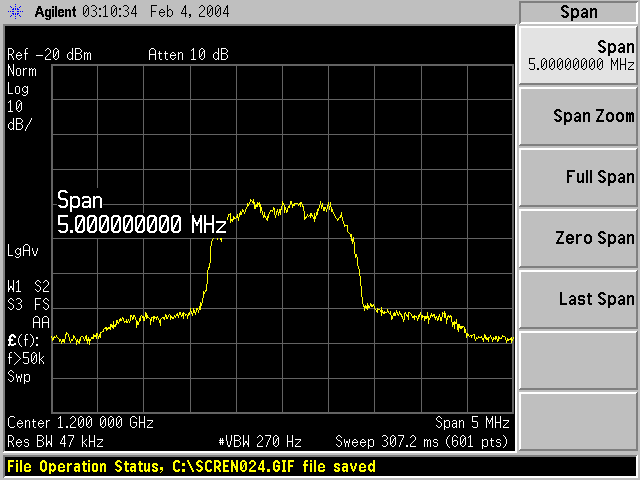
\includegraphics[width=110mm]{SAsingleNoSideLobe.png}}
    \caption{Spectrum of single-band signal with low-energy side lobes. Measured by Agilent E4440A PSA Series Spectrum Analyzer.}
    \label{fig:SAsingleNoSideLobe}
  \end{center}
\end{figure}


\begin{figure}[tpb]
  \begin{center}
    \centerline{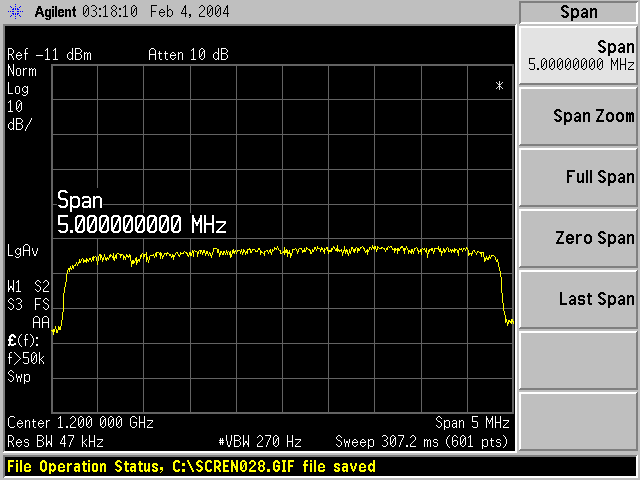
\includegraphics[width=110mm]{SASingleLargeBand.png}}
    \caption{Spectrum of single-band signal with large bandwidth. Measured by Agilent E4440A PSA Series Spectrum Analyzer.}
    \label{fig:SASingleLargeBand}
  \end{center}
\end{figure}


To determine the value of $\beta$, there is an assumption that all sub-bands with the information signal have the same signal level and all sub-bands with the side lobe signal have the same signal level. Suppose the number of sub-bands with information signal is $n_1$, and the number of sub-bands with side lobe is $n_2$. The achievable region of $\left( {{n_1},{n_2}} \right)$ is
\begin{align}
\mathcal{R} =\left\{ {\left( {{n_1},{n_2}} \right):{n_1},{n_2} \in {\mathbb{Z}^ + };{n_1} + {n_2} \le 16} \right\}.
\end{align}
Let
\begin{align}
m_2=\alpha m_1, \quad \alpha<1.
\end{align}
Then
\begin{align}
{m_0} = \frac{{{n_1}{m_1} + {n_2}{m_2}}}{{{n_1} + {n_2}}} = \frac{{{n_1}{m_1} + {n_2}\alpha {m_1}}}{{{n_1} + {n_2}}} = \frac{{{n_1} + {n_2}\alpha }}{{{n_1} + {n_2}}}{m_1}
\end{align}
\begin{align}
{S_0} &= \sqrt {\frac{1}{{{n_1} + {n_2} - 1}}\left[ {{n_1}{{\left( {{m_1} - {m_0}} \right)}^2} + {n_2}{{\left( {{m_2} - {m_0}} \right)}^2}} \right]}&\\
&= \sqrt {\frac{1}{{{n_1} + {n_2} - 1}}\left[ {{n_1}{{\left( {{m_1} - \frac{{{n_1} + {n_2}\alpha }}{{{n_1} + {n_2}}}{m_1}} \right)}^2} + {n_2}{{\left( {\alpha {m_1} - \frac{{{n_1} + {n_2}\alpha }}{{{n_1} + {n_2}}}{m_1}} \right)}^2}} \right]}&\\
&={m_1}\left( {1 - \alpha } \right)\sqrt {\frac{{{n_1}{n_2}}}{{\left( {{n_1} + {n_2} - 1} \right)\left( {{n_1} + {n_2}} \right)}}}.&
\label{S0finalvalue}
\end{align}

From (\ref{DecisionCretia}) and (\ref{S0finalvalue})
\begin{align}
\beta  &\le \frac{{{m_0} - {E_i}}}{{{S_0}}}&\\
&= \frac{{\frac{{{n_1} + {n_2}\alpha }}{{{n_1} + {n_2}}}{m_1} - \alpha {m_1}}}{{{m_1}\left( {1 - \alpha } \right)\sqrt {\frac{{{n_1}{n_2}}}{{\left( {{n_1} + {n_2} - 1} \right)\left( {{n_1} + {n_2}} \right)}}} }}&\\
&= \sqrt {\frac{{{n_1}\left( {{n_1} + {n_2} - 1} \right)}}{{{n_2}\left( {{n_1} + {n_2}} \right)}}}.&
\end{align}
Considering all the possible values of $n_1$ and $n_2$ in the achievable region, we can determine
\begin{align}
\mathop {\min }\limits_{\left( {{n_1},{n_2}} \right) \in {\cal R}} \left\{ {\sqrt {\frac{{{n_1}\left( {{n_1} + {n_2} - 1} \right)}}{{{n_2}\left( {{n_1} + {n_2}} \right)}}} } \right\}=\frac{1}{4}
\end{align}
when $n_1=1$ and $n_2=15$. As a result $\beta \le \frac{1}{4}$ detects all the side lobes based on the criteria of (\ref{DecisionCretia}). A more conservative value of $\beta = \frac{1}{8}$ is chosen for the spectrum analyzer.

\section{Performance of the Spectrum Analyzer}

\subsection{System Setup}
The test setup for assessment of the spectrum analyzer is shown in Figure~\ref{fig:SpectrumAnalyzerSetup}. One USRP is used as a receiver for the spectrum analyzer, and another two USRPs are used as interference sources. The distance between the spectrum analyzer and the interference source is about 3 feet. A Marconi Instruments 2041 low noise signal generator is also used to generate tone interference as shown in Figure \ref{fig:SAsingleTone}
\begin{figure}[tpb]
  \begin{center}
    \centerline{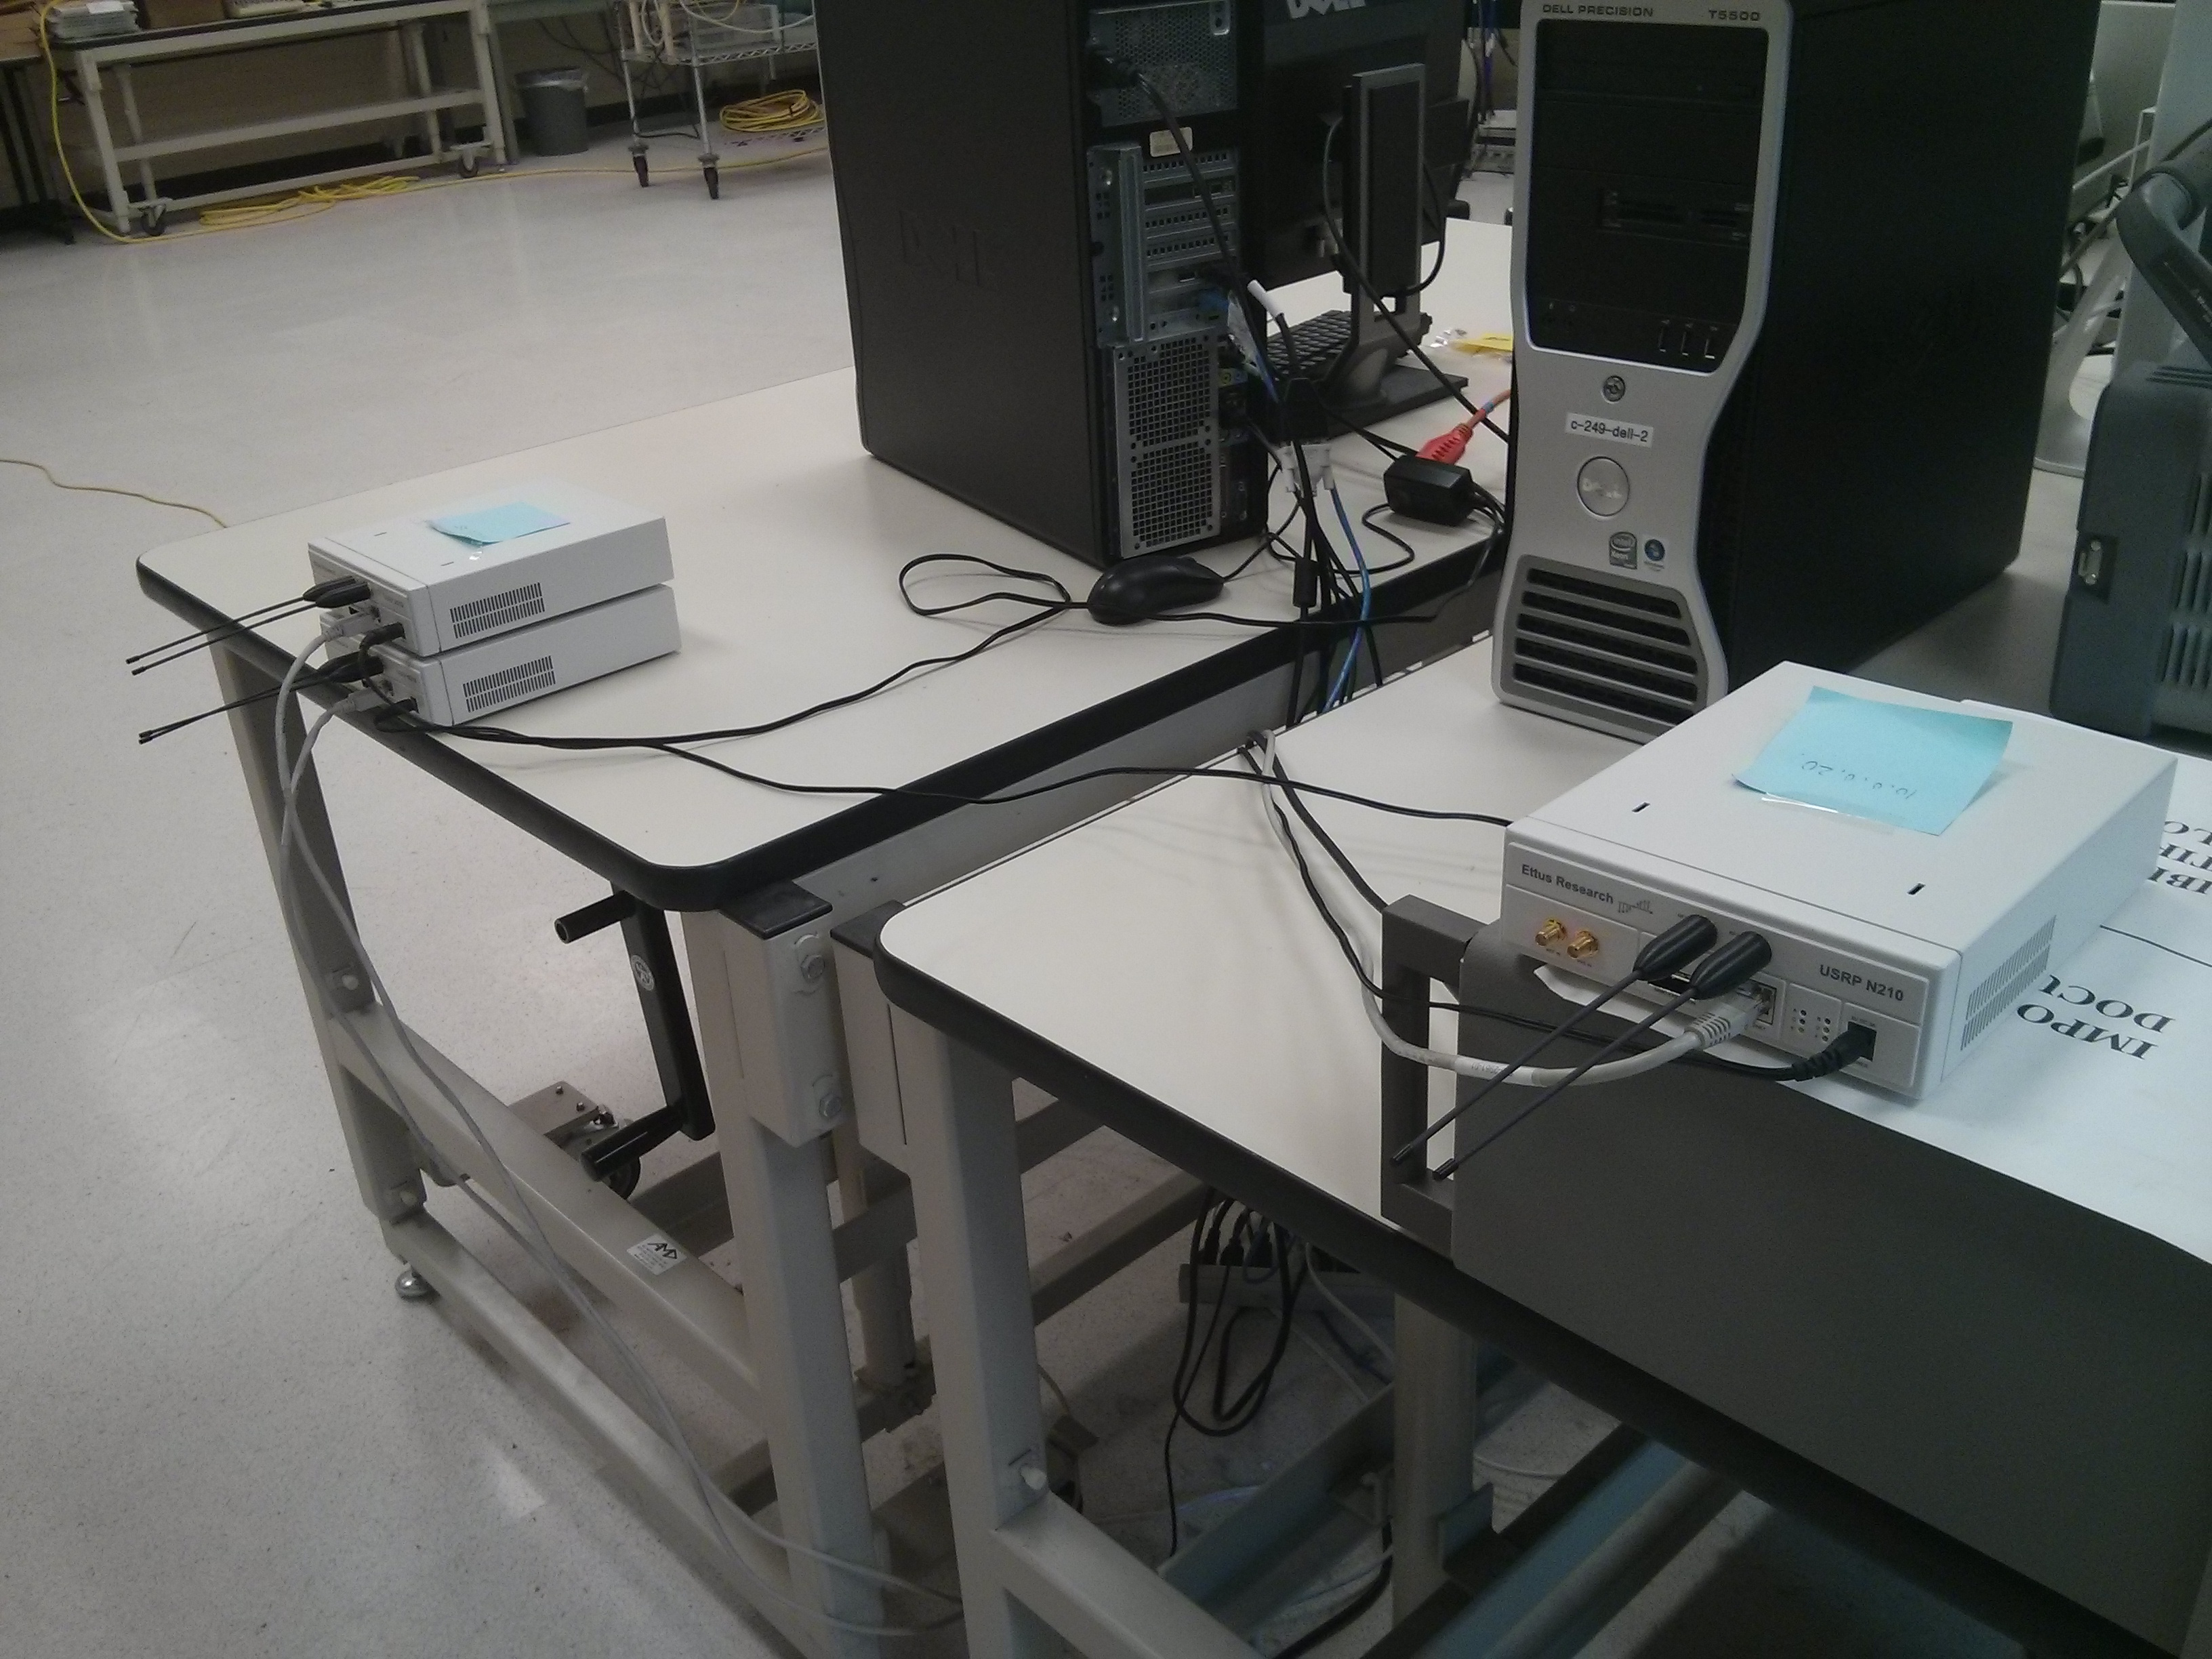
\includegraphics[width=160mm]{SpectrumAnalyzerSetup.jpg}}
    \caption{Setup of spectrum analyzer (right) and interference sources (left). Separation distance is approximately 3 feet.}
    \label{fig:SpectrumAnalyzerSetup}
  \end{center}
\end{figure}

\subsection{Testing Result}
Table \ref{tbl:SAtestResult} lists the detection results of the spectrum analyzer with different types of interference or cooperators' signal, including a sinusoid tone as shown in Figure \ref{fig:SAsingleTone},  a single-carrier signal with side lobes (SSSL) as shown in Figure \ref{fig:SAsinglewithSideLob}, a single-carrier signal with low-energy side lobes (SSLSL) as shown in Figure \ref{fig:SAsingleNoSideLobe}, a single-band signal with large bandwidth (SSLB) as shown in Figure \ref{fig:SASingleLargeBand}, and a two-band signal with side lobes (TSSL) as shown in Figure \ref{fig:SAtwoSignal}. Let 1 denote that a sub-band is available for use and 0 denote the sub-band is our cooperator's signal. The spectrum analyzer is run 1000 times, and the rate of sub-band availability is calculated.

Test results show that the spectrum analyzer can detect the interference and ignore the side lobes. There is small rate of missed detection, such as the sensing results of sub-band 9 and 10 for SSLSL, which is tolerable.

%\begin{table}[tpb]
%  \begin{center}
%    \caption{TEST RESULT��OF SPECTRUM ANALYZER \label{tbl:SAtestResult}}
%    \begin{tabularx}{0.85\textwidth}{llr} \toprule
%      {Test No.}  &  Interference type     &  Availble sub-band  \\ \midrule
%1     &{\begin{tabular}{@{}l@{}} Tone\end{tabular}}                               &1111111011111111 \\\bottomrule
%2     &{\begin{tabular}{@{}l@{}} Single-band signal\\ with side lobes\end{tabular}}           &1111100000011111 \\\bottomrule
%3     &{\begin{tabular}{@{}l@{}} Single-band signal\\ with low-energy side lobes\end{tabular}} &1111100000011111 \\\bottomrule
%4     &{\begin{tabular}{@{}l@{}} Single-band signal\\ with large bandwidth \end{tabular}}      &0000000000000000 \\\bottomrule
%5     &{\begin{tabular}{@{}l@{}} Two-band signal \\with side lobes\end{tabular}}               &1000000110000001 \\ \bottomrule
%    \end{tabularx}
%  \end{center}
%\end{table}

\begin{table}
\centering
    \caption{TEST RESULT: RATE OF SUB-BAND AVAILABILITY (1000 TRAILS) \label{tbl:SAtestResult}}
    \begin{tabular}{cccccc} \toprule
      {Sub-band index}
      &{\begin{tabular}{@{}l@{}} Tone\end{tabular}}
      &{\begin{tabular}{@{}l@{}} SSSL\end{tabular}}
      &{\begin{tabular}{@{}l@{}} SSLSL\end{tabular}}
      &{\begin{tabular}{@{}l@{}} SSLB \end{tabular}}
      &{\begin{tabular}{@{}l@{}} TSSL\end{tabular}}   \\ \bottomrule
1     &1.000    &1.000  &1.000  &0.163  &1.000  \\\bottomrule
2     &1.000    &1.000  &1.000  &0      &1.000  \\\bottomrule
3     &1.000    &1.000  &1.000  &0      &0.984  \\\bottomrule
4     &1.000    &1.000  &1.000  &0      &1.000  \\\bottomrule
5     &1.000    &1.000  &1.000  &0      &0      \\\bottomrule
6     &1.000    &1.000  &1.000  &0      &0      \\\bottomrule
7     &1.000    &0      &0      &0      &0      \\\bottomrule
8     &0        &0      &0      &0      &0      \\\bottomrule
9     &1.000    &0      &0.014  &0      &1.000  \\\bottomrule
10    &1.000    &0      &0.014  &0      &1.000  \\\bottomrule
11    &1.000    &1.000  &1.000  &0      &0      \\\bottomrule
12    &1.000    &1.000  &1.000  &0      &0      \\\bottomrule
13    &1.000    &1.000  &1.000  &0      &0      \\\bottomrule
14    &1.000    &1.000  &1.000  &0      &0.427  \\\bottomrule
15    &1.000    &1.000  &1.000  &0      &1.000  \\\bottomrule
16    &1.000    &1.000  &1.000  &0.361  &1.000  \\\bottomrule
    \end{tabular}
\end{table}



\begin{figure}[tpb]
  \begin{center}
    \centerline{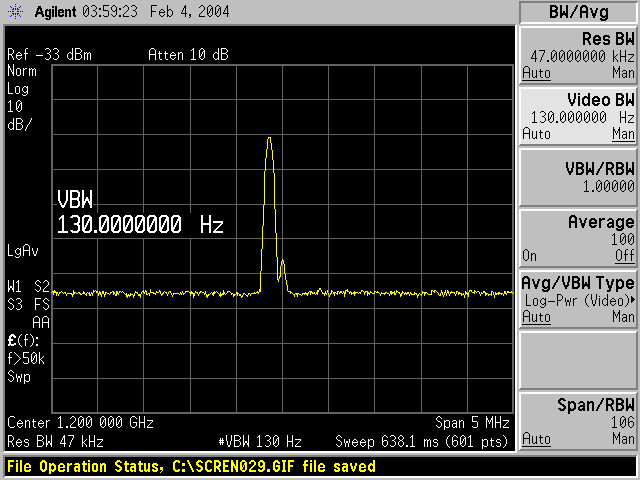
\includegraphics[width=110mm]{SAsingleTone.png}}
    \caption{Spectrum of sinusoid signal. Signal generated by Marconi instruments 2041 low noise signal generator. Measured by Agilent E4440A PSA Series Spectrum Analyzer.}
    \label{fig:SAsingleTone}
  \end{center}
\end{figure}


\begin{figure}[tpb]
  \begin{center}
    \centerline{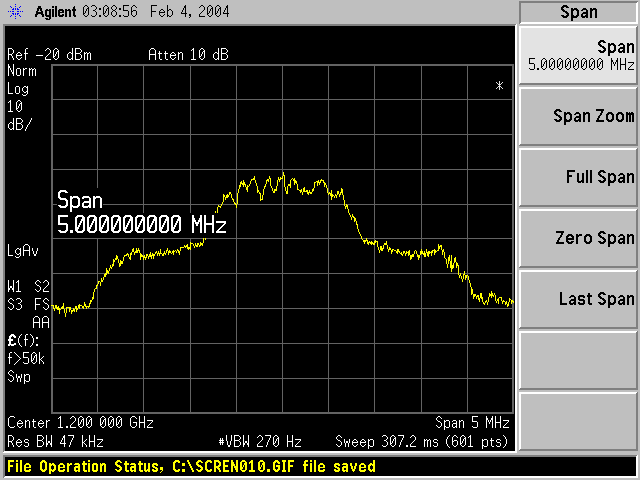
\includegraphics[width=110mm]{SAsinglewithSideLob.png}}
    \caption{Spectrum of single-band signal with side lobes. Measured by Agilent E4440A PSA Series Spectrum Analyzer.}
    \label{fig:SAsinglewithSideLob}
  \end{center}
\end{figure}


\begin{figure}[tpb]
  \begin{center}
    \centerline{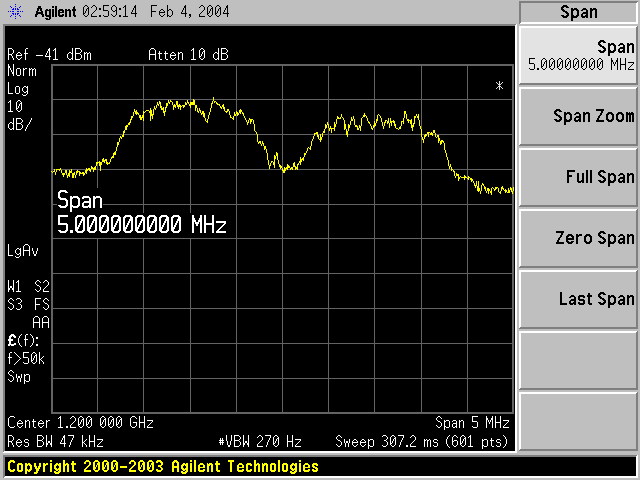
\includegraphics[width=110mm]{SAtwoSignal.png}}
    \caption{Spectrum of two-band signal with side lobes. Measured by Agilent E4440A PSA Series Spectrum Analyzer.}
    \label{fig:SAtwoSignal}
  \end{center}
\end{figure}








%
% Chapter 6
%

\chapter{TIME DIVISION DUPLEX SYSTEM}
\label{chap:TDD}
As discussed in Chapter \ref{chap:strategyAnalysis}, feedback is incorporated into our strategies. This chapter focuses on the implementation of TDD with USRP and GNU Radio.

\begin{figure}[tpb]
  \begin{center}
    \centerline{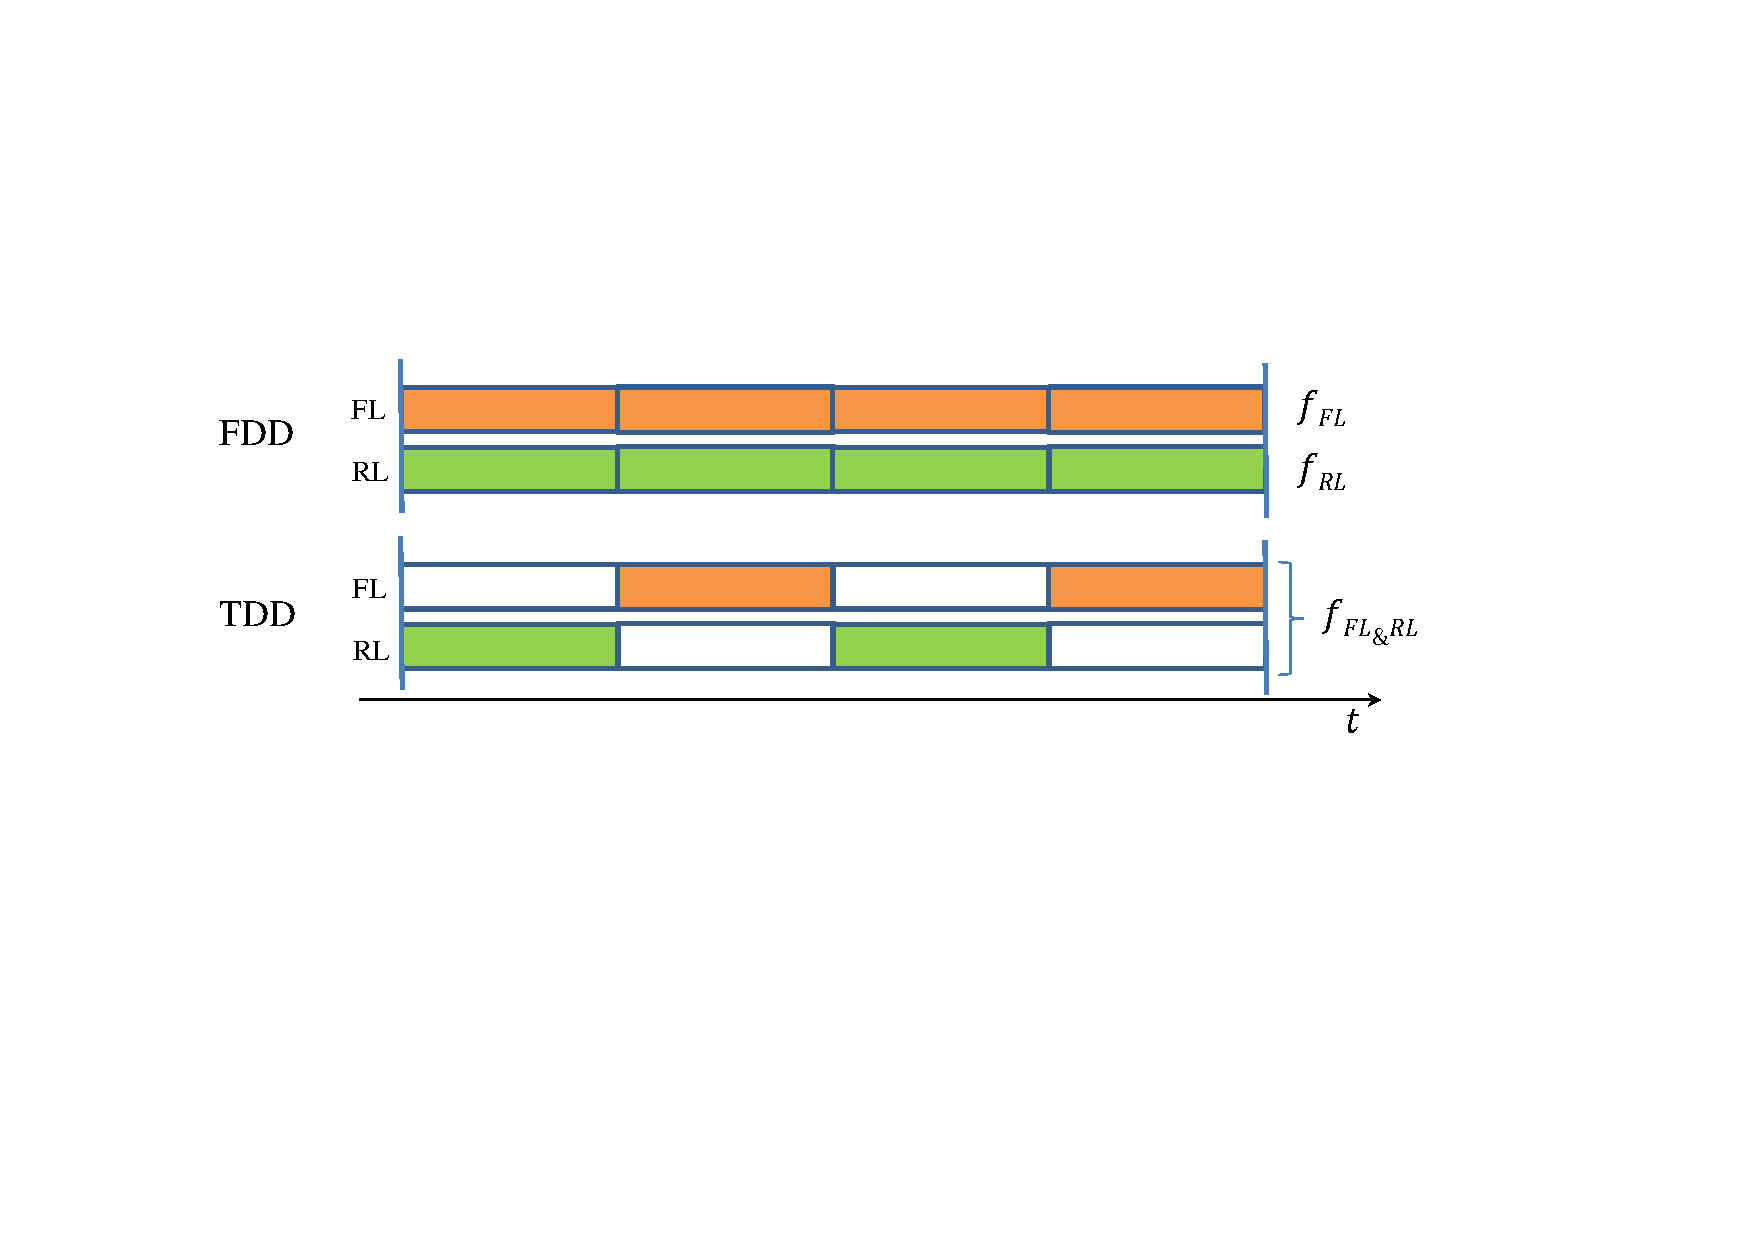
\includegraphics[width=140mm]{TDDandFDD.pdf}}
    \caption{Illustration of TDD and FDD. FL stands for forward link, and RL stands for reverse link.}
    \label{fig:TDDandFDD}
  \end{center}
\end{figure}

\section{Introduction to TDD}
In the TDD method, a single frequency band is assigned to both the transmitter and the receiver, and the forward link and reverse link use the same spectrum at different times as shown in Figure~\ref{fig:TDDandFDD}. There are some advantages of TDD over FDD \cite{MoonbLinkTDDFDD}:
\begin{itemize}

\item In TDD, a guard band is not required to separate the forward link and reverse link. However, a guard time is necessary for synchronization purposes. Generally, the spectrum cost of the guard time is less than that of the guard band in FDD in terms of spectrum efficiency.

\item In TDD, only one set of parameters or one physical layer is needed, because of the symmetry of forward link and reverse link. However, in FDD, two sets of parameters have to be tuned for both links or two physical layers have to be developed for each link.

\item The TDD scheme can dynamically allocate the proportion of time slots assigned to forward link and reverse link while it is difficult for FDD implementations to dynamically adjust the proportion of spectrum usage for both links.
\end{itemize}

Examples of technologies using TDD include Universal Mobile Telecommunications System (UMTS) 3G supplementary air interfaces, TD-CDMA for mobile telecommunications, TD-SCDMA 3G mobile telephony air interface, Chinese TD-LTE 4G and TD-SCDMA 3G mobile communications, DECT wireless telephony, IEEE 802.16 WiMAX, PACTOR, and digital enhanced cordless telecommunications (DECT) wireless telephony \cite{wikipediaDuplex, TechoPediaTDD}.

\section{Design and Implementation of TDD System}
In a TDD system, the key issue is the time synchronization between source and destination. To achieve good synchronization, the transmission time and receiving time for both the source and destination should be controlled. The USRP N210 has a mode called burst mode that can be used to control the transmission time. In software, stream tags in GNU Radio are used to control the burst mode of USRP.
\subsection{Introduction to Stream Tags and USRP Burst Mode}
A stream tag is an isosynchronous data stream that runs parallel to the main data stream in GNU Radio \cite{GNURadioStreamTags}. A stream tag can be generated by a signal processing block and can be attached to a particular data sample. The stream tag moves along with the data sample to the following blocks until it reaches a sink block or is forced to stop propagating by another signal processing block, which can be set up by the programmer.

A stream tag consists of a key, a value, and a source ID. The key identifies the type of information inside the streams tag. The value is the message carried by the stream tag. The source ID defines the name of the block creating the stream tag. The key, value, and source ID are all PMTs (Polymorphic Types) defined in GNU Radio. In practice, the type can be used to store anything, and it also has simple conversion methods for common data types such as boolean, long, or vector in C++. For details of PMTs, please refer to \cite{GNURadioPolymorphicType}.

Each data processing block can call a GNU Radio system function to read all of the stream tags contained in incoming samples. The block can identify the stream tags by their source ID and key.

USRP Burst Mode can be controlled by three tags with fixed keys, defined by the USRP hardware and GNU Radio software, which are \texttt{tx\_time}, \texttt{tx\_sob} and \texttt{rx\_sob} defined by USRP and GNU. The value of the \texttt{tx\_time} stream tag defines the start time of the first data sample in a burst transmission round. The start time is the USRP time maintained in the USRP hardware and counted in seconds from  the instant that the USRP is powered on. The \texttt{tx\_sob} tag orders the USRP transmitter to be in burst mode starting with the next data sample, and the \texttt{rx\_sob} stream tag tells the USRP transmitter to stop burst mode and to switch to normal transmission mode with the next data sample.

Another system stream tag defined by USRP and GNU Radio is \texttt{rx\_time}, which tells the USRP time at which the sample is sent from the USRP to the GNU Radio through the Ethernet interface. It is sent only once for the first data sample when system just starts or overflow happens. Overflow is unique to the software receiver. When overflow occurs, the processing speed of the host PC cannot keep up with the received data from the USRP. Consequently, the buffer in the USRP overflows, and the data samples are dropped. The stream tag \texttt{rx\_time} is very helpful for the implementation of a TDD system, which will be explained in the following section.

\subsection{Tagger and Muter}
As shown in Figure \ref{fig:MuterTaggerFlowgraph}, GNU Radio signal processing blocks called Tagger and Muter have been developed to control the TDD operation. The Tagger manages the burst transmission, and the Muter decides whether data samples are forwarded to the following blocks based on the TDD state. The Muter also keeps track of the USRP time at the GNU Radio software level.

\begin{figure}[tpb]
  \begin{center}
    \centerline{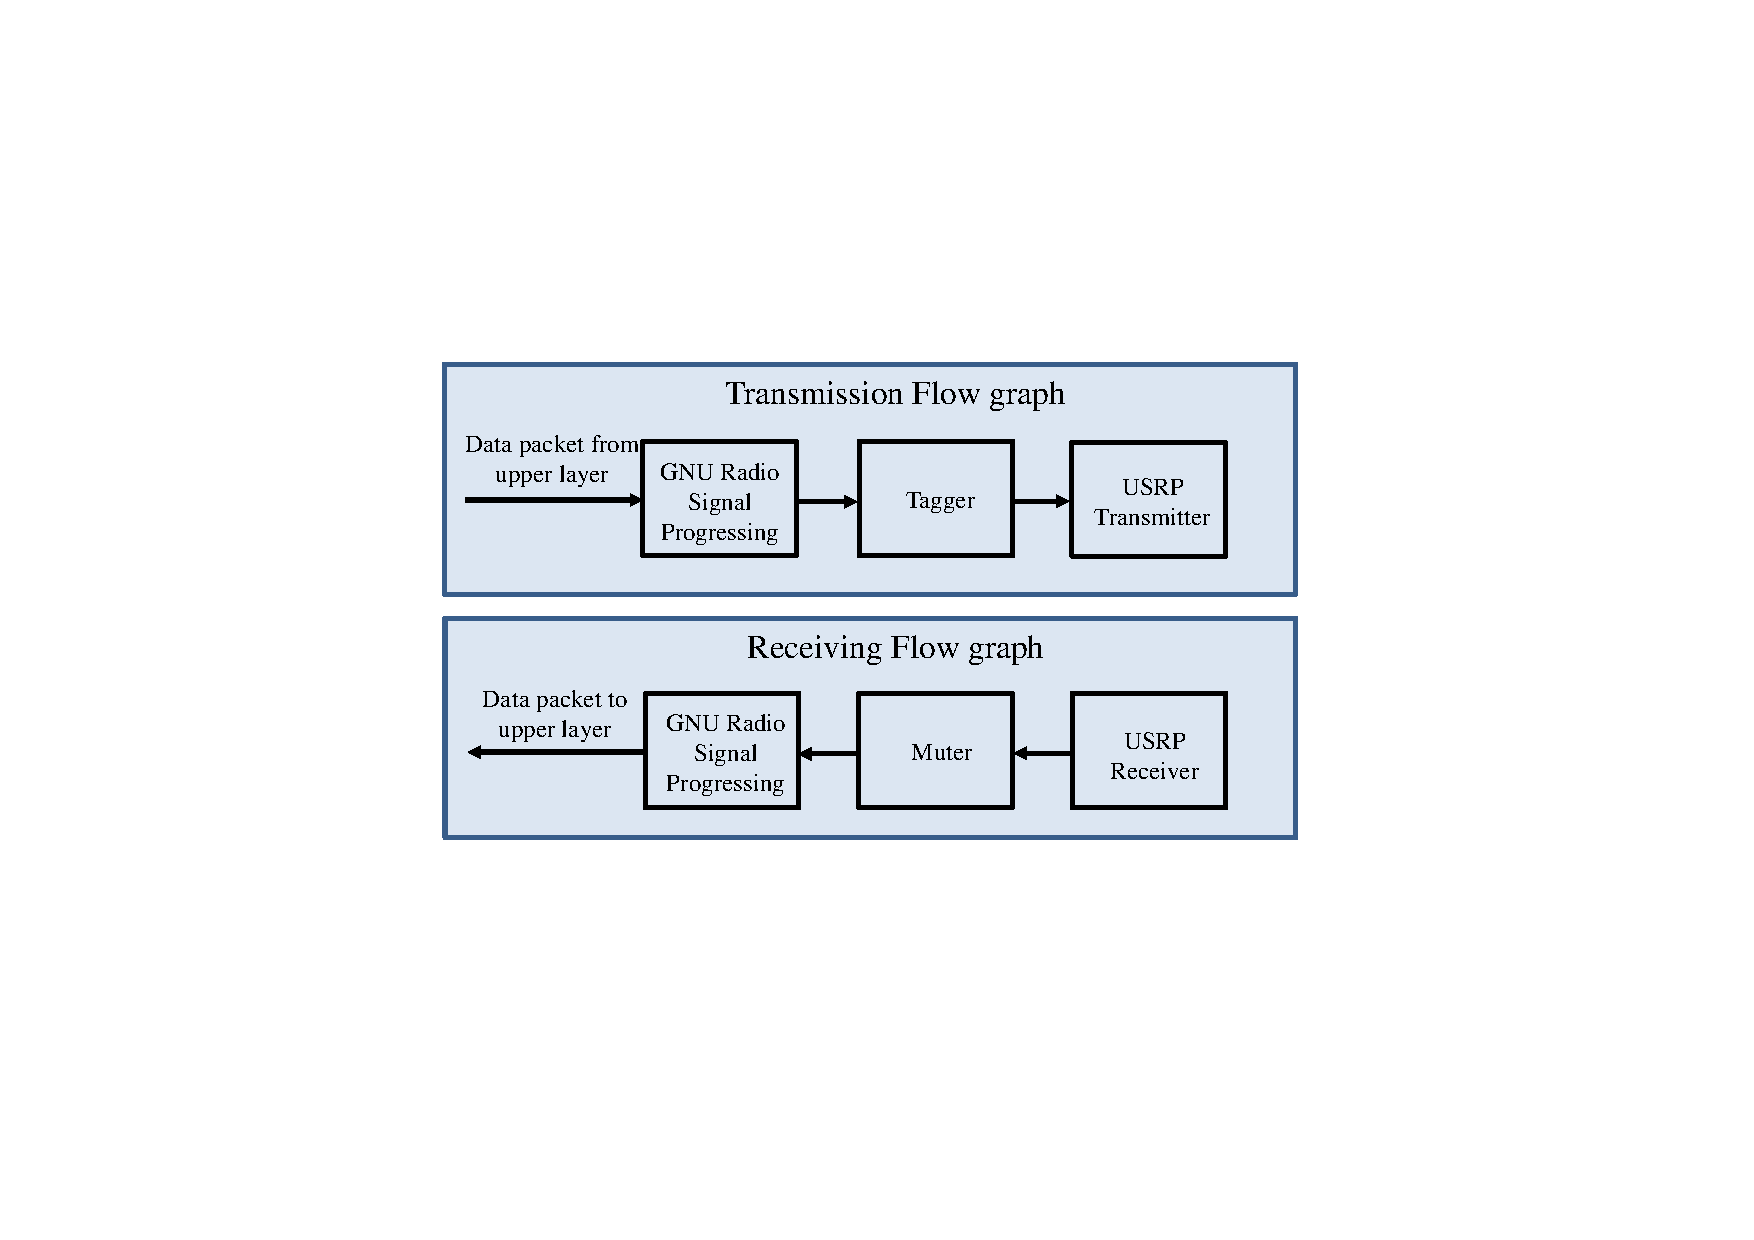
\includegraphics[width=140mm]{MuterTaggerFlowgraph.pdf}}
    \caption{Tagger and Muter in the transmission and receiving flow graphs.}
    \label{fig:MuterTaggerFlowgraph}
  \end{center}
\end{figure}

\subsubsection{Tagger}
The Tagger controls the burst transmission by stream tags \texttt{tx\_time}, \texttt{tx\_sob} and \texttt{rx\_sob}. Let the idle period be the receiving period of a TDD cycle and define the idle duration to be the time of an idle period. The Tagger calculates the idle duration and the burst duration based upon the number of samples from prior blocks and the sampling rate of the USRP, e.g., 5 MHz.

During system initialization, an upper layer function obtains the USRP time through the function \texttt{get\_time\_now}, and sets an initial burst time based on the current USRP time. The Tagger then automatically updates the next burst time based on the calculated idle and burst durations. There is also an interface in Tagger to receive adjusted burst times from the Muter so that the TDD burst cycle can be dynamically adjusted.
\subsubsection{Muter}
The Muter connects directly to the USRP source block. There is a software clock in Muter to keep track of the USRP time. The Muter waits for the \texttt{rx\_time} tag. Once it receives a \texttt{rx\_time} tag, the Muter will update its software clock time to the USRP time contained in the stream tag, which we will denote as $t_s$. The Muter will continue to update its clock based on $t_s$, the number of samples received after the tag ($N_S$), and the sampling rate ($R_S$), according to
\begin{align}
{t_c} = {t_s} + \frac{{{N_S}}}{{{R_S}}}.
\end{align}

The Muter controls each TDD cycle with an estimate of the USRP hardware time by forwarding and blocking data samples at the appropriate time. In an operation defined as Disable Muter, the Muter forwards the data samples to next signal processing block in the receiving mode. In the complementary operation defined as Enable Muter, the Muter blocks the data samples in transmission mode by setting the received data samples to be 0, which prevents receiving data sent from the same antenna.

A TDD sub-frame, and a physical-layer packet have been defined in Section \ref{comptititveStrategy}. Each sub-frame requires 1.74 milliseconds to transmit. In the header of every reverse link physical-layer packet, there is one byte called ``sub-frame'' left indicating how many TDD sub-frames remain in the current receiving mode in a TDD cycle. The Muter can adjust its samples that need to be forwarded in the current Muter enabling state.

However, signal processing delay occurs from the time a physical-layer packet is received in the Muter to the time the ``sub-frame left'' information is decoded and passed to the Muter. The delay can be estimated in the physical layer. The Muter adds stream tags containing the current USRP time in the data samples. After the physical-layer packet has been decoded, the physical layer obtains the current USRP time from the Muter and compares it with the time contained in the stream tags to calculate the packet processing delay. The calculated delay is passed to the Muter. Then the Muter can adjust the TDD cycle based on the ``sub-frame left'' information and the signal processing delay. At the same time, the Muter can also calculate the next start time of a burst transmission and pass it to the Tagger. The Tagger will adjust its next start time accordingly.

The TDD timing adjustment feature of the Muter can be set to be ON or OFF.

\subsection{Two-way TDD Timing Adjustment vs. One-way TDD Timing Adjustment}
In GNU Radio and the USRP, if the data has been pushed to the buffer in the USRP, its burst time cannot be changed. Therefore, the data in the next burst transmission has to be prepared in advance. There is also variable signal processing time and Ethernet transmission time in the GNU Radio and USRP. A typical value would be several milliseconds. As a result, the burst data needs to be prepared one TDD cycle ahead of the burst start time.

Suppose a TDD cycle starts with the receiving period. The timing adjustment in the Muter is in effect immediately while the timing adjustment in the Tagger will not be in effect until next TDD cycle, because the burst data in the current TDD cycle has been sent to the USRP and cannot be changed.

Ideally, two-way TDD timing adjustment is preferable. However, the preparation of burst data in advance makes this impossible. Figure \ref{fig:TDDtwoWayAdjustment} shows an example of two-way TDD timing adjustment. Guard time is not considered here. Suppose that starting from time $t_0$, the timing of the destination has a $\Delta t$ offset with respect to the source. Then the adjustment scheme starts to work. However, from $t_1$ to $t_2$, the adjustment does not fulfill a good synchronization between the source and destination. Actually, the adjustment process will just repeat the situation from $t_1$ to $t_2$ forever. Consequently, two-way TDD timing adjustment fails.


\begin{figure}[tpb]
  \begin{center}
    \centerline{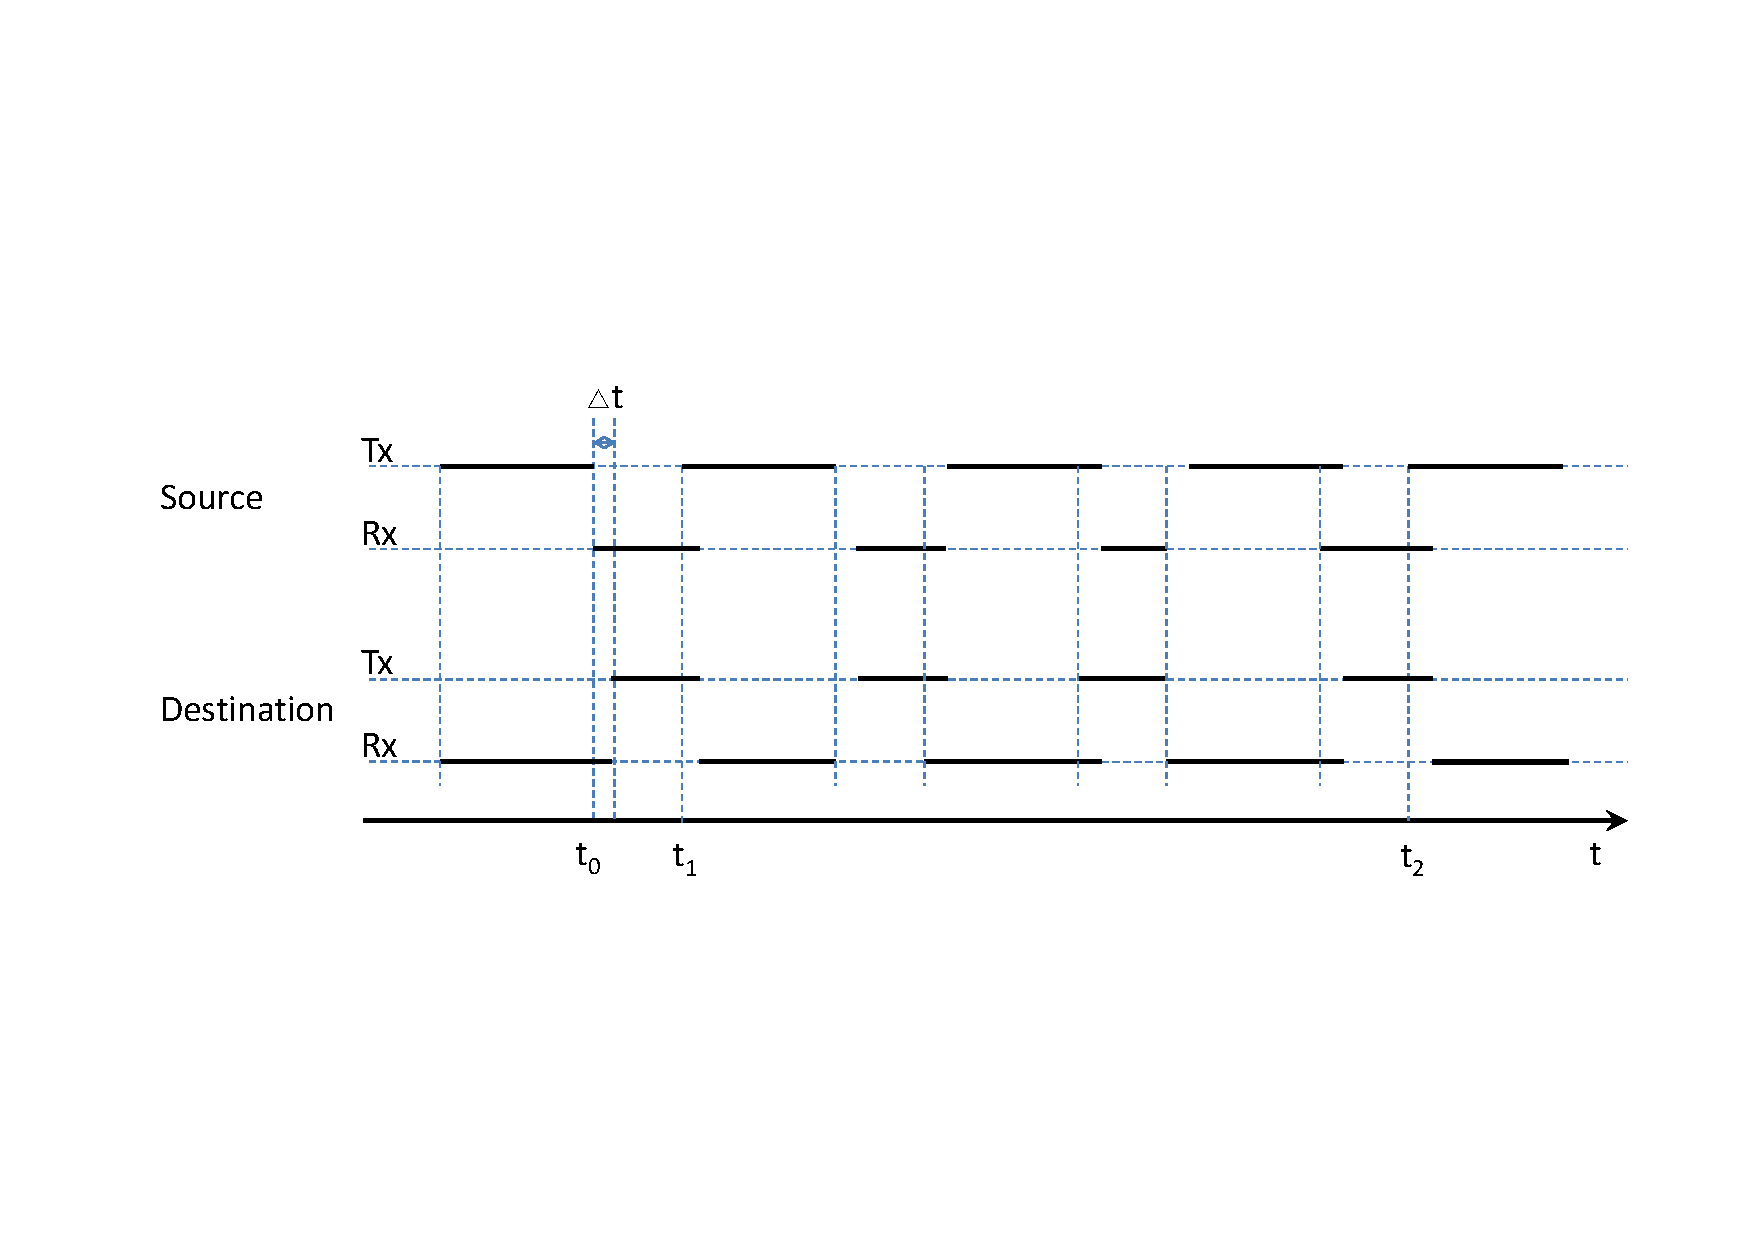
\includegraphics[width=160mm]{TDDtwoWayAdjustment.pdf}}
    \caption{Example of two-way TDD timing adjustment.}
    \label{fig:TDDtwoWayAdjustment}
  \end{center}
\end{figure}


\begin{figure}[tpb]
  \begin{center}
    \centerline{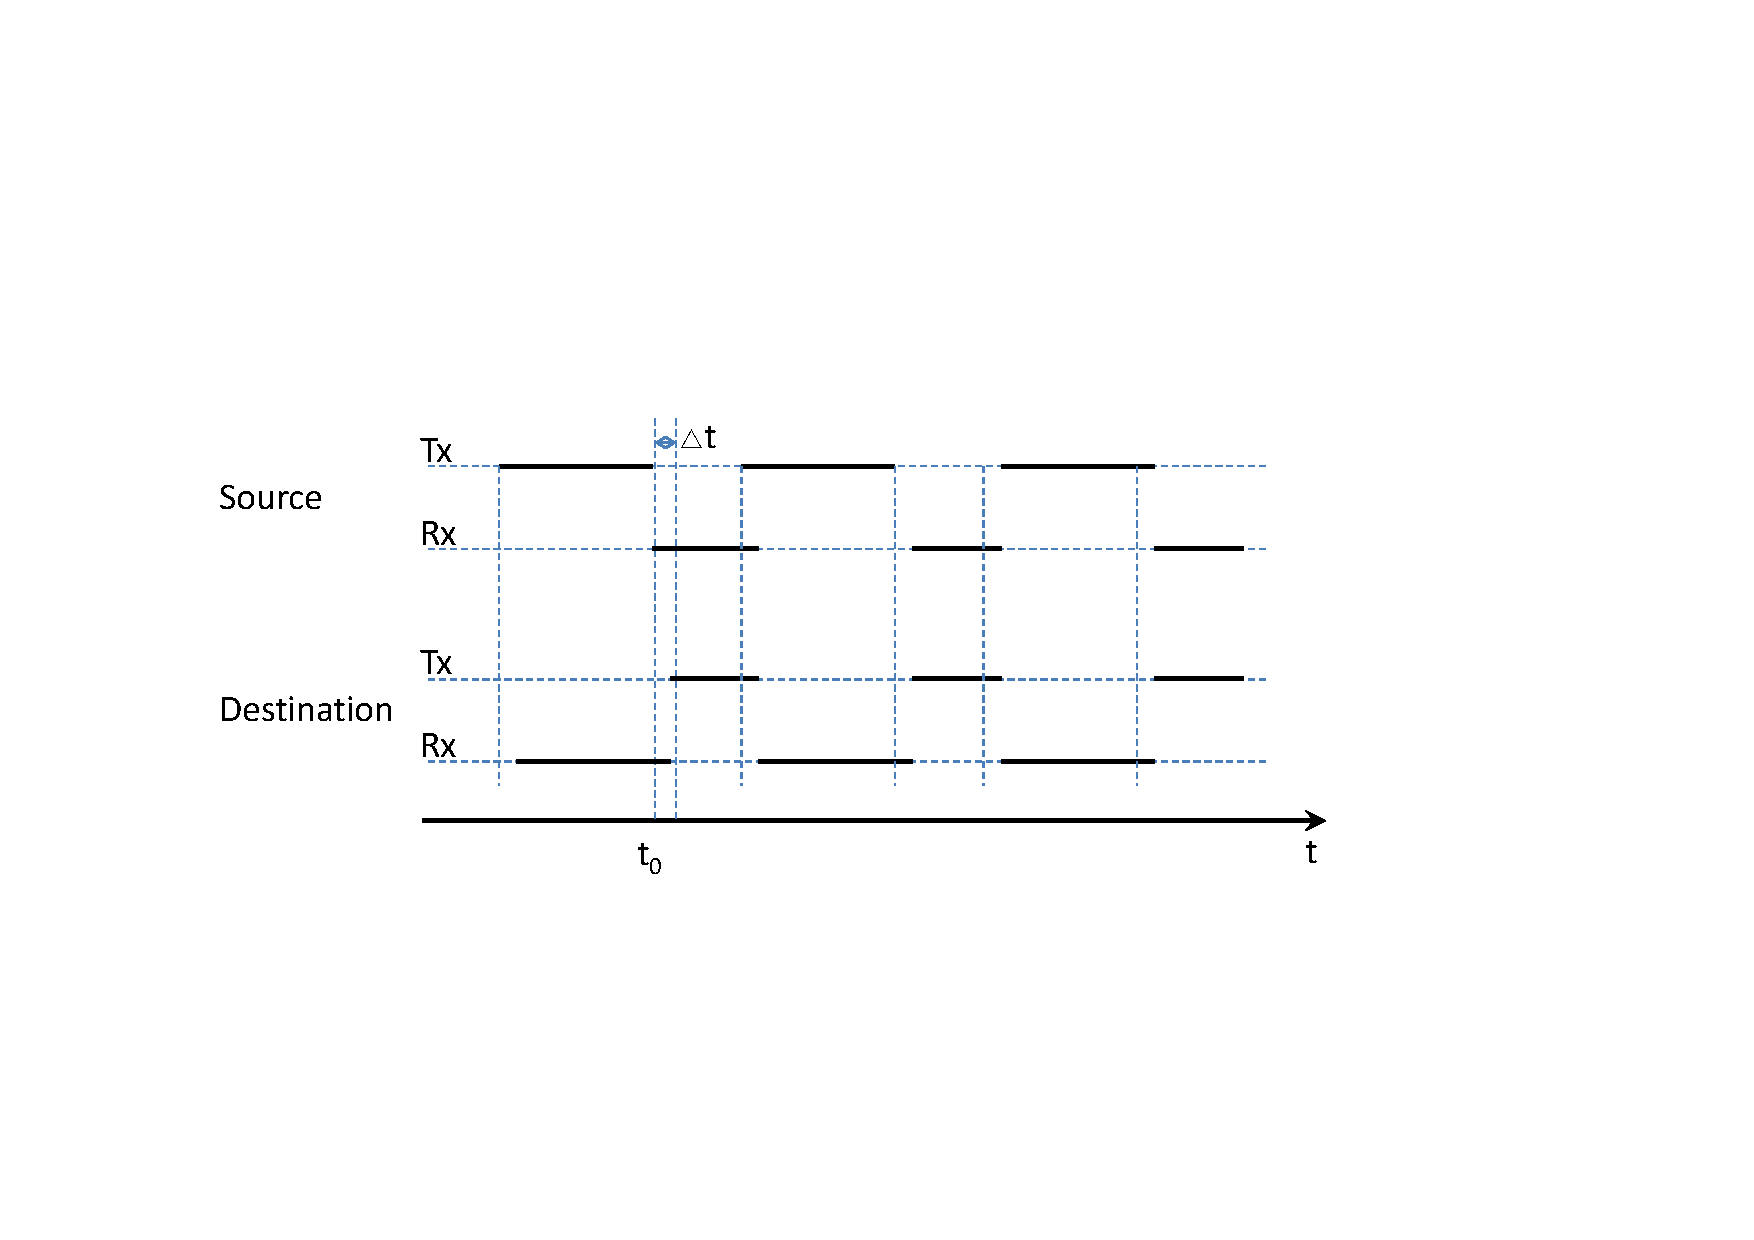
\includegraphics[width=160mm]{TDDoneWayAdjustment.pdf}}
    \caption{Example of one-way TDD timing adjustment. The source adjusts according the data sent from the destination.}
    \label{fig:TDDoneWayAdjustment}
  \end{center}
\end{figure}

Now consider the one-way TDD timing adjustment example as shown in Figure \ref{fig:TDDoneWayAdjustment}. Suppose that starting from time $t_0$, the timing of the destination has a $\Delta t$ offset with respect to the source. The synchronization recovers completely within one TDD cycle.

As a result, one-way TDD timing adjustment is the only option, but a natural question is whether the one-way timing adjustment should be conducted in the forward link or the reverse link.

\subsection{TDD Timing Adjustment in Forward Link vs. Reverse Link}
\label{TDDTimingAdjustemntForwardReverse}
Synchronization for TDD totally depends on the timing adjustment. If more than one physical-layer packet is successfully received, the TDD timing adjustment of TDD can be completed because every physical-layer packet contains the ``sub-frames left'' information. The success probability of TDD timing adjustment relies on the link quality. As Figure~\ref{fig:CompetitiveNodeGeometryFinalRound} suggests, the reverse link has much higher SIR than the forward link, and it is therefore much more reliable than the forward link. As a result, the TDD timing adjustment was chosen to be conducted in the reverse link as discussed in Chapter \ref{chap:strategy}.

However, the transmission time of the reverse link is smaller than that of the forward link, because the ultimate goal is to transmit as many packets as possible in the forward link. If the timing offset between the source and destination is larger than the receiving period of the source node, the TDD timing can never be synchronized as shown in Figure \ref{fig:TDDOneWayAdjFailure}.

A potential solution is to let the receiver of the source wait until it receives at least one useful physical-layer packet, but there are two problems. First, there will not be enough time to prepare the burst data. Second, if the reverse link is not good, our radio has no signal in the air during most of the waiting period. Then our competitor can transmit at higher speed.

\begin{figure}[tpb]
  \begin{center}
    \centerline{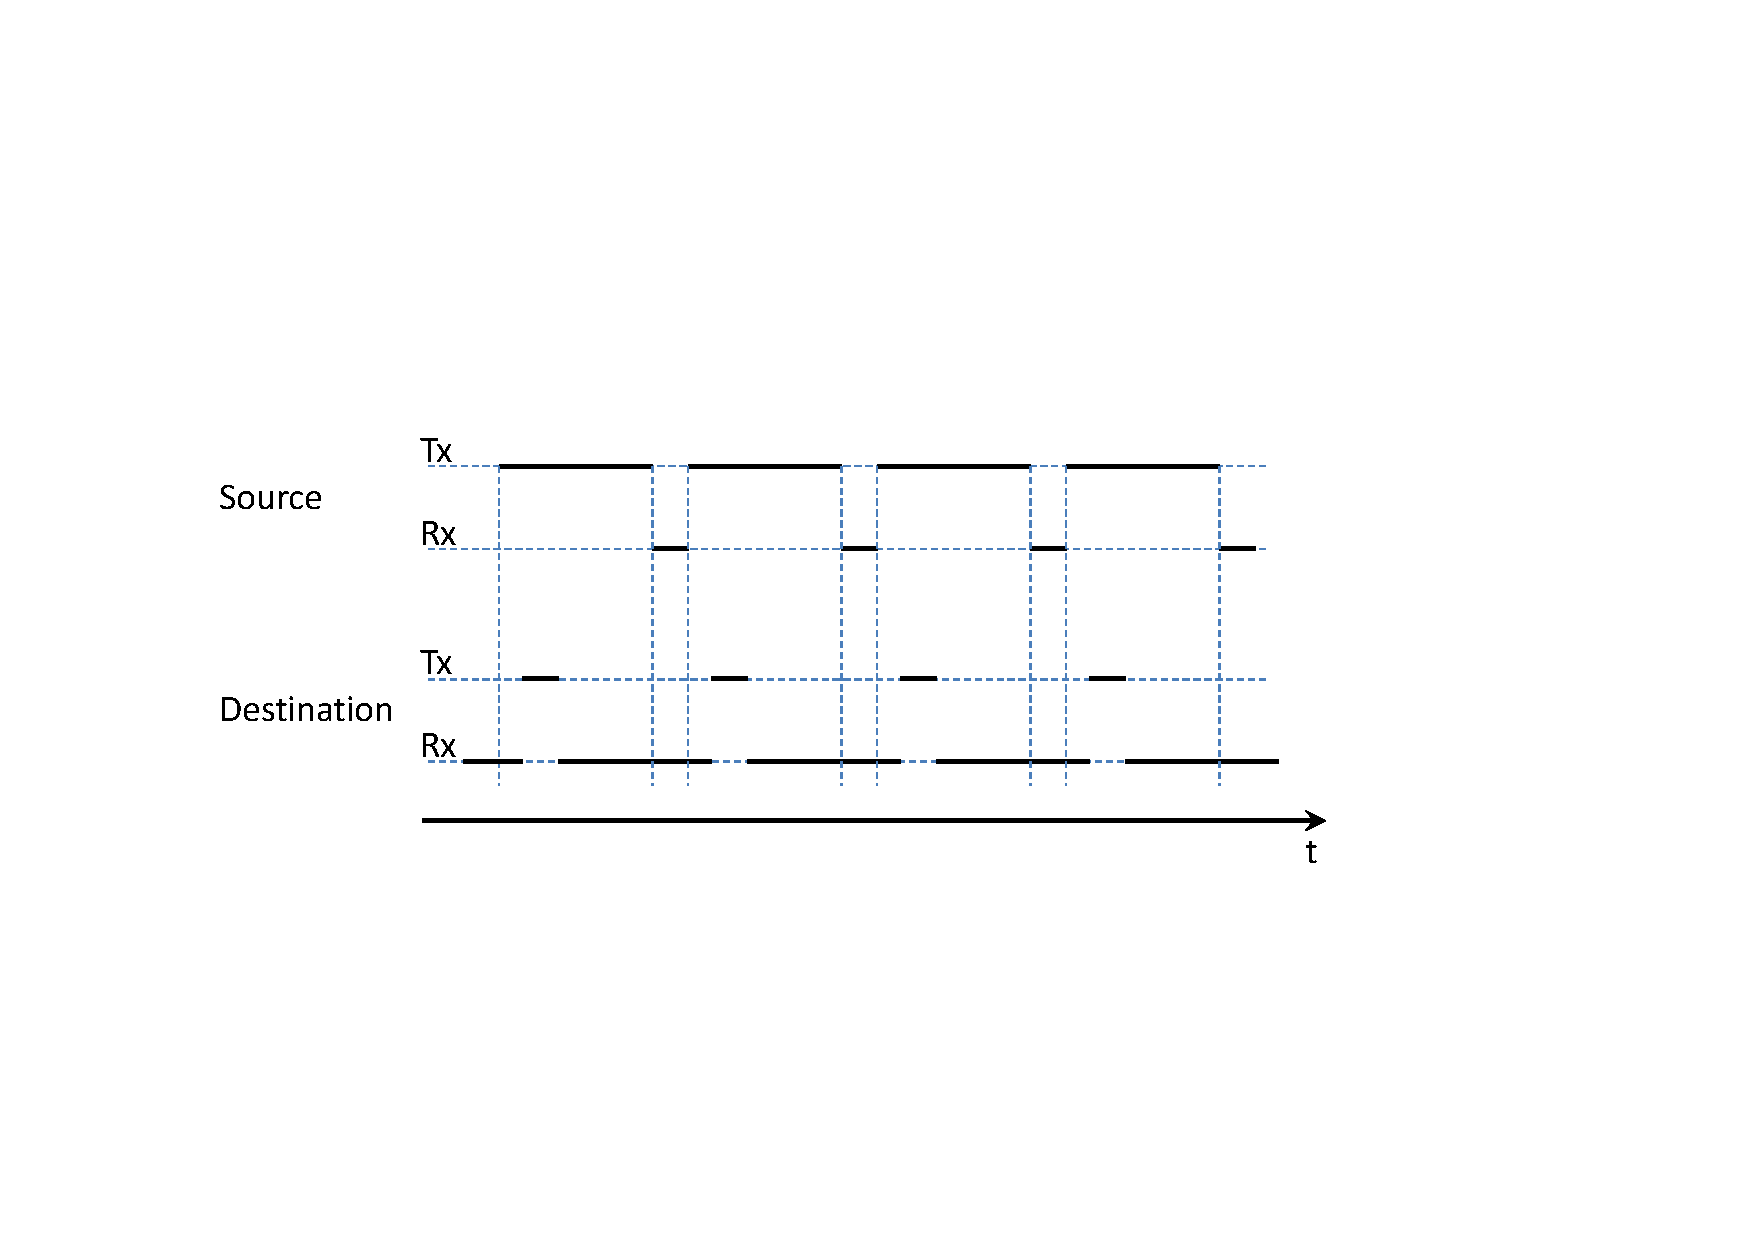
\includegraphics[width=160mm]{TDDOneWayAdjFailure.pdf}}
    \caption{Example of one-way TDD timing adjustment failure in the reverse link. The source adjusts according to the data from the destination.}
    \label{fig:TDDOneWayAdjFailure}
  \end{center}
\end{figure}

This problem can be solved by setting the initial state of the source and destination.
\subsection{Initial State}
There are two potential initial states in TDD system. First, the source and destination will start to transmit in TDD mode immediately after the radios start. The TDD synchronization depends on the one-way TDD timing adjustment. However, as discussed in Section \ref{TDDTimingAdjustemntForwardReverse}, the TDD timing can never be synchronized if the timing offset between the source and destination is larger than the receiving period of the source node as illustrated in  Figure \ref{fig:TDDOneWayAdjFailure}. If the TDD timing adjustment is conducted in the forward link, there will not be a synchronization problem.

The second potential initial state involves the destination starting to transmit in TDD mode initially while the source waits in receiving state for a valid physical-layer packet. After receiving a valid physical-layer packet, the source reverts to its normal TDD mode and adjusts its TDD cycle according to the physical-layer packets received in the reverse link.

For the DARPA Spectrum Challenge, the second initial state was chosen for our system. Figure \ref{fig:TDDflowchart} illustrates the flow graph of the TDD designed. For the TDD used in the DARPA Spectrum Challenge, $m_1=100$ and $m_2=10$.
\begin{figure}[tpb]
  \begin{center}
    \centerline{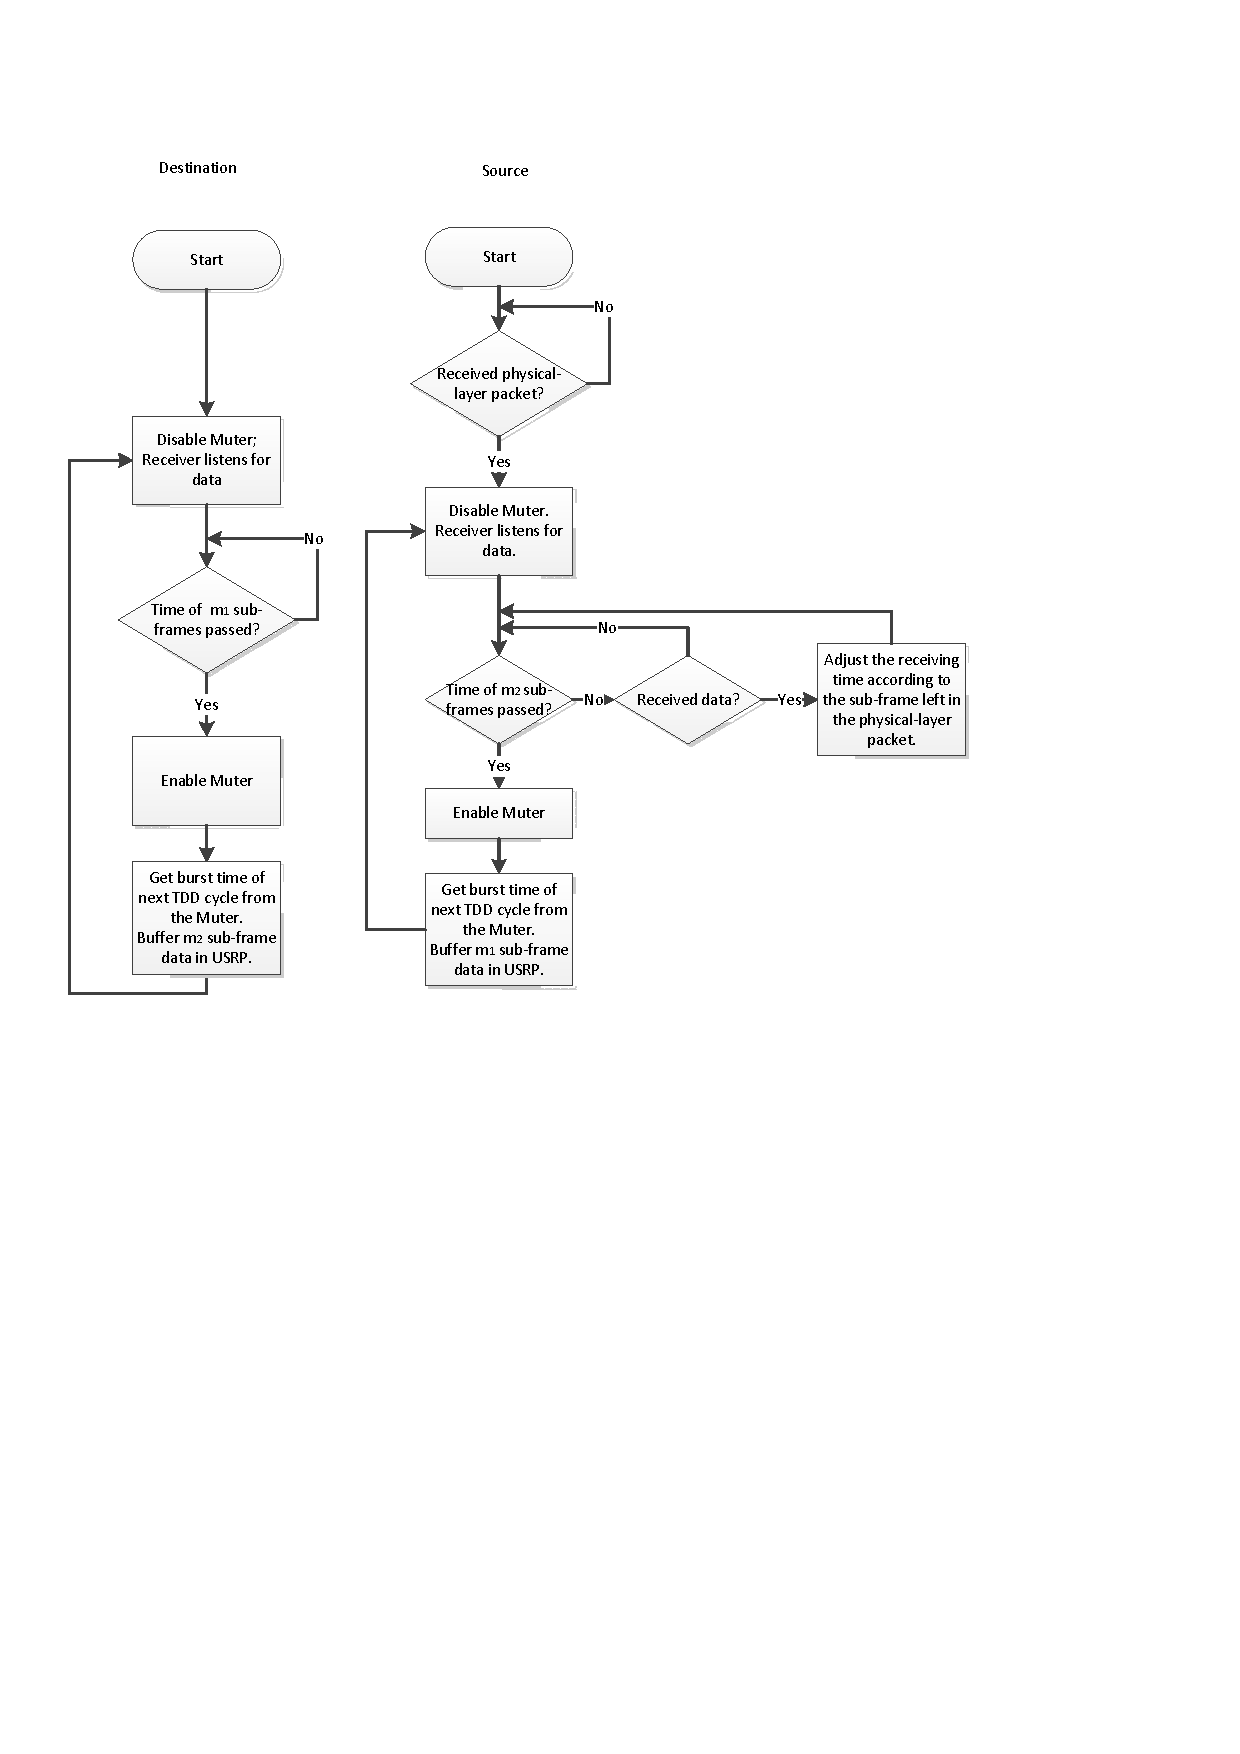
\includegraphics[width=160mm]{TDDflowchart.pdf}}
    \caption{TDD flow graph.}
    \label{fig:TDDflowchart}
  \end{center}
\end{figure}



%%%%%%%%%%%%%%%%%%%%%%%%%%%%%%%%%%%%%%%%%%%%%%%%%%%%%%%%%%%%%%%%%%%%%%%%

%
% Chapter 7
%

\chapter{PERFORMANCE AND DISCUSSION}
\label{chap:performance}
\section{Performance of the cooperative spectrum access system}
We assess the performance of the cooperative spectrum access system with three experiments. First, out cooperative radio runs with static interference. Second, three of our cooperative radios running together. Finally, our cooperative radio runs with other teams' radios in the DARPA Spectrum Challenge.

\subsection{Static Interference}
\label{staticInterference}
\begin{figure}[tpb]
  \begin{center}
    \centerline{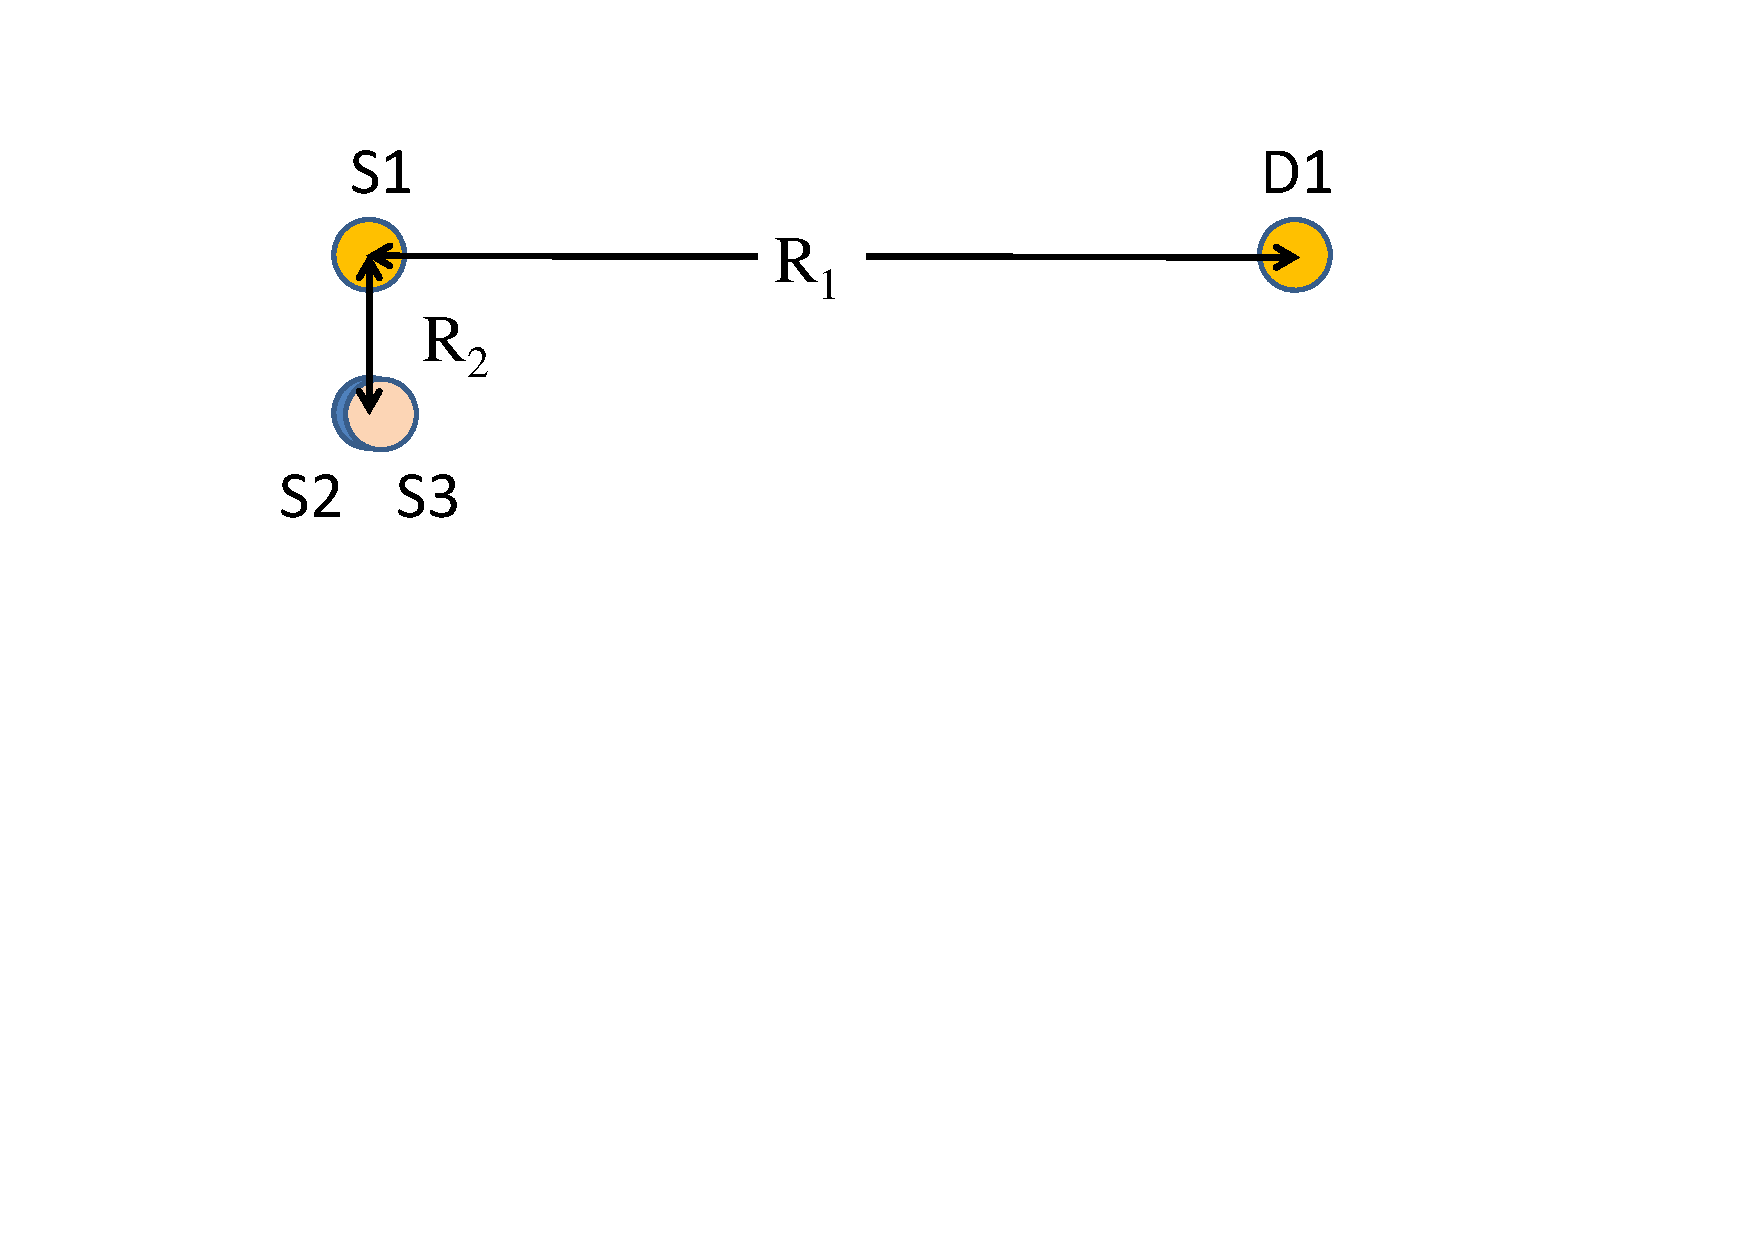
\includegraphics[width=160mm]{CoopTestNodeAssignment.pdf}}
    \caption{Radio geometry for the cooperative static interference test. The distances are roughly $R_1 = 30$ feet and $R_2 = 3$ feet}
    \label{fig:CoopTestNodeAssignment}
  \end{center}
\end{figure}

The cooperative radio is run with different types of interference, including a single-carrier signal with low-energy side lobes (SSLSL) as shown in Figure \ref{fig:SAsingleNoSideLobe}, a sinusoid tone as shown in Figure \ref{fig:SAsingleTone},  a single-carrier signal with side lobes (SSSL) as shown in Figure \ref{fig:SAsinglewithSideLob}, and a two-band signal with side lobes (TSSL) as shown in Figure \ref{fig:SAtwoSignal}.

The setup is as in Figure~\ref{fig:CoopTestNodeAssignment}. S1 is our source and D1 is our destination. S2 and S3 are the interference sources. The distance between the source and interference nodes ($R_1$) is 30 feet, and the distance between the source and destination $R_2$ is 3 feet. The distance between the source and destination is limited by the length of the Ethernet cable between the USRP and computer.

Table \ref{tbl:COOPTestResultsStatic} shows the test results. The metric is the amount of time (in seconds) for the cooperative radio to successfully transmit 15000 packets. Without interference, the average transmission time is 39.1 seconds, which is consistent with our physical layer parameters. Ideally, the transmission time with interference should be inversely proportional to the number of available sub-bands, but the test results for situation with interference are slightly worse, which suggests that there is potential improvement in the physical-layer.

\begin{table}[tpb]
\centering
    \caption{TEST RESULT (IN SECONDS): COOPERATIVE RADIO WITH STATIC INTERFERENCE (10 TESTS) \label{tbl:COOPTestResultsStatic}}
    \begin{tabular}{cccccc} \toprule
      {Test No.}
      &{No interference}
      &{\begin{tabular}{@{}l@{}} Tone\end{tabular}}
      &{\begin{tabular}{@{}l@{}} SSSL\end{tabular}}
      &{\begin{tabular}{@{}l@{}} SSLSL\end{tabular}}
      &{\begin{tabular}{@{}l@{}} TSSL\end{tabular}}   \\ \bottomrule
1                    &42.1	&46.2	&80.1	&62.7	&187.7 \\ \hline
2                    &40.9	&40.9	&78.7	&62.7	&212.0 \\ \hline
3                    &41.9	&41.2	&95.4	&59.1	&202.6 \\ \hline
4                    &38.0  &41.0	&101.1	&62.0	&193.4 \\ \hline
5                    &38.3	&42.2	&98.1	&57.5	&222.9 \\ \hline
6                    &35.9	&46.0	&82.6	&57.2	&182.6 \\ \hline
7                    &42.0	&48.8	&99.0	&57.6	&183.0 \\ \hline
8                    &38.2	&46.0	&78.8	&62.4	&182.7 \\ \hline
9                    &37.2	&46.0	&100.2	&58.9	&218.0 \\ \hline
10                   &36.1	&41.7	&93.4	&59.9	&182.2 \\\bottomrule
{\begin{tabular}{@{}c@{}} Available Number \\of sub-bands\end{tabular}}
                     &16	&15	    &12	    &12  	&7     \\ \hline
Mean                 &39.1	&44.0	&90.74	&60.0	&196.7 \\ \hline
Standard Deviation   &2.4	&2.9	&9.5	&2.3	&16.0  \\\bottomrule
    \end{tabular}
\end{table}



\subsection{Three Cooperative Radios Running Together}
\begin{table}[tpb]
  \begin{center}
    \caption{TEST RESULT (IN SECONDS): THREE COOPERATIVE RADIOS RUNNING TOGETHER (10 TESTS) \label{tbl:COOPTestResultsSelf}}
    \begin{tabular}{cc} \toprule
    {Test No.}        & {\begin{tabular}{@{}c@{}} Time to transmit \\ 15000 packets (seconds)\end{tabular}}\\ \midrule
1     &147.3\\
2     &88.9  \\
3     &132.0 \\
4     &98.0 \\
5     &115.1\\
6     &107.7\\
7     &96.4\\
8     &166.5\\
9     &110.1\\
10    &119.5\\\bottomrule
Mean                 &118.1 \\
Standard Deviation   &24.2  \\\bottomrule
    \end{tabular}
  \end{center}
\end{table}

The setup is also shown in Figure~\ref{fig:CoopTestNodeAssignment} with $R_1 = 30$ feet and $R_2 = 3$ feet. Each pair of cooperative radio is set up to use the different preambles to avoid synchronization problems. The metric is the amount of time for S1 and D1 to transmit 15000 packets. Test results are shown in Table \ref{tbl:COOPTestResultsSelf}. The average transmission time for one radio running with two other cooperative radios, is 118.1 seconds, which is almost 3 times of that without interference as shown in Table \ref{tbl:COOPTestResultsStatic}. This test result demonstrates that our cooperative radio can cooperate well with radios running the same protocol.

\subsection{Running with Other Teams' Radios}
The final test is in the Final Tournament of the DARPA Spectrum Challenge. The rules have been introduced in Chapter \ref{chap:backgound}. Our cooperative radio ranked first in the preliminary group, as show in Table \ref{tbl:COOPTestResultsDSCPreDeteils} and Table \ref{tbl:COOPTestResultsDSCPreSummary}. In the Semifinal group, our cooperative radio ranked third as shown in Table \ref{tbl:COOPTestResultsDSCSemiFinalDeteils} and Table \ref{tbl:COOPTestResultsDSCSemiFinalSummary} \cite{DSCFinalEventResults}.

\begin{table}[tpb]
  \begin{center}
    \caption{TEST RESULT: COOPERATIVE RADIO WITH OTHER TEAMS' RADIOS (PRELIMINARY ROUND DETAILS) \label{tbl:COOPTestResultsDSCPreDeteils}}
    \begin{tabular}{c lllccc} \toprule
Round  &{Player 1} &{Player 2} &{Player 3} &{P1 Score} &{P2 Score} &{P3 Score} \\ \bottomrule
1    &WSL-NEU &WINBOT &{\begin{tabular}{l} Wireless \\ Infidels\end{tabular}}      &18990  &18990  &14166 \\ \hline
2    &WINBOT  &WSL-NEU  &{\begin{tabular}{l} Notre \\Spectrum\end{tabular}}        &18703  &18703  &18271 \\ \hline
3    &{\begin{tabular}{l} Wireless \\ Infidels\end{tabular}} &{\begin{tabular}{l} Notre \\Spectrum\end{tabular}} &WINBOT &16739  &23678  &23678 \\ \hline
4    &{\begin{tabular}{l} Notre \\Spectrum\end{tabular}}      &{\begin{tabular}{l} Wireless \\ Infidels\end{tabular}} &WSL-NEU     &20633  &16627  &20633  \\ \bottomrule
    \end{tabular}
  \end{center}
\end{table}


\begin{table}[tpb]
  \begin{center}
    \caption{TEST RESULT: COOPERATIVE RADIO WITH OTHER TEAMS' RADIOS (PRELIMINARY ROUND SUMMARY) \label{tbl:COOPTestResultsDSCPreSummary}}
    \begin{tabular}{lc} \toprule
       {Group B} &{Total Score} \\ \bottomrule
WSL-NEU             &58326 \\ \hline
WINBOT              &61371 \\ \hline
Wireless Infidels   &47532 \\ \hline
Notre Spectrum      &62582  \\ \bottomrule
First:              &Notre Spectrum  \\ \hline
Second:             &WSL-NEU       \\  \bottomrule
    \end{tabular}
  \end{center}
\end{table}

\begin{table}[tpb]
  \begin{center}
    \caption{TEST RESULT: COOPERATIVE RADIO WITH OTHER TEAMS' RADIOS (SEMIFINAL ROUND DETAILS) \label{tbl:COOPTestResultsDSCSemiFinalDeteils}}
    \begin{tabular}{clllccc} \toprule
Round &{Player 1} &{Player 2} &{Player 3} &{P1 Score} &{P2 Score} &{P3 Score} \\ \bottomrule
1   &{\begin{tabular}{l} Notre \\Spectrum\end{tabular}}      &VT-Hume    &Tenn Tech  &20291  &15077  &20291 \\ \hline
2   &VT-Hume     &{\begin{tabular}{l} Notre \\Spectrum\end{tabular}}     &MarmotE        &18993  &21413  &21413 \\ \hline
3   &Tenn Tech   &MarmotE            &VT-Hume        &24471  &24471  &17912 \\ \hline
4   &MarmotE     &Tenn Tech      &{\begin{tabular}{l} Notre \\Spectrum\end{tabular}} &19597  &19597  &13877  \\ \bottomrule
    \end{tabular}
  \end{center}
\end{table}

\begin{table}[tpb]
  \begin{center}
    \caption{TEST RESULT: COOPERATIVE RADIO WITH OTHER TEAMS' RADIOS (SEMIFINAL ROUND SUMMARY) \label{tbl:COOPTestResultsDSCSemiFinalSummary}}
    \begin{tabular}{lc} \toprule
       {Group F} &{Total Score} \\ \bottomrule
Notre Spectrum  &55581 \\ \hline
VT-Hume         &51982 \\ \hline
Tenn Tech Tel   &64359 \\ \hline
MarmotE         &65481  \\ \bottomrule
First:          &MarmotE  \\ \hline
Second:         &Tenn Tech Tel      \\  \bottomrule
    \end{tabular}
  \end{center}
\end{table}

%\FloatBarrier
\section{Performance of the competitive spectrum access system}
\begin{figure}[tpb]
  \begin{center}
    \centerline{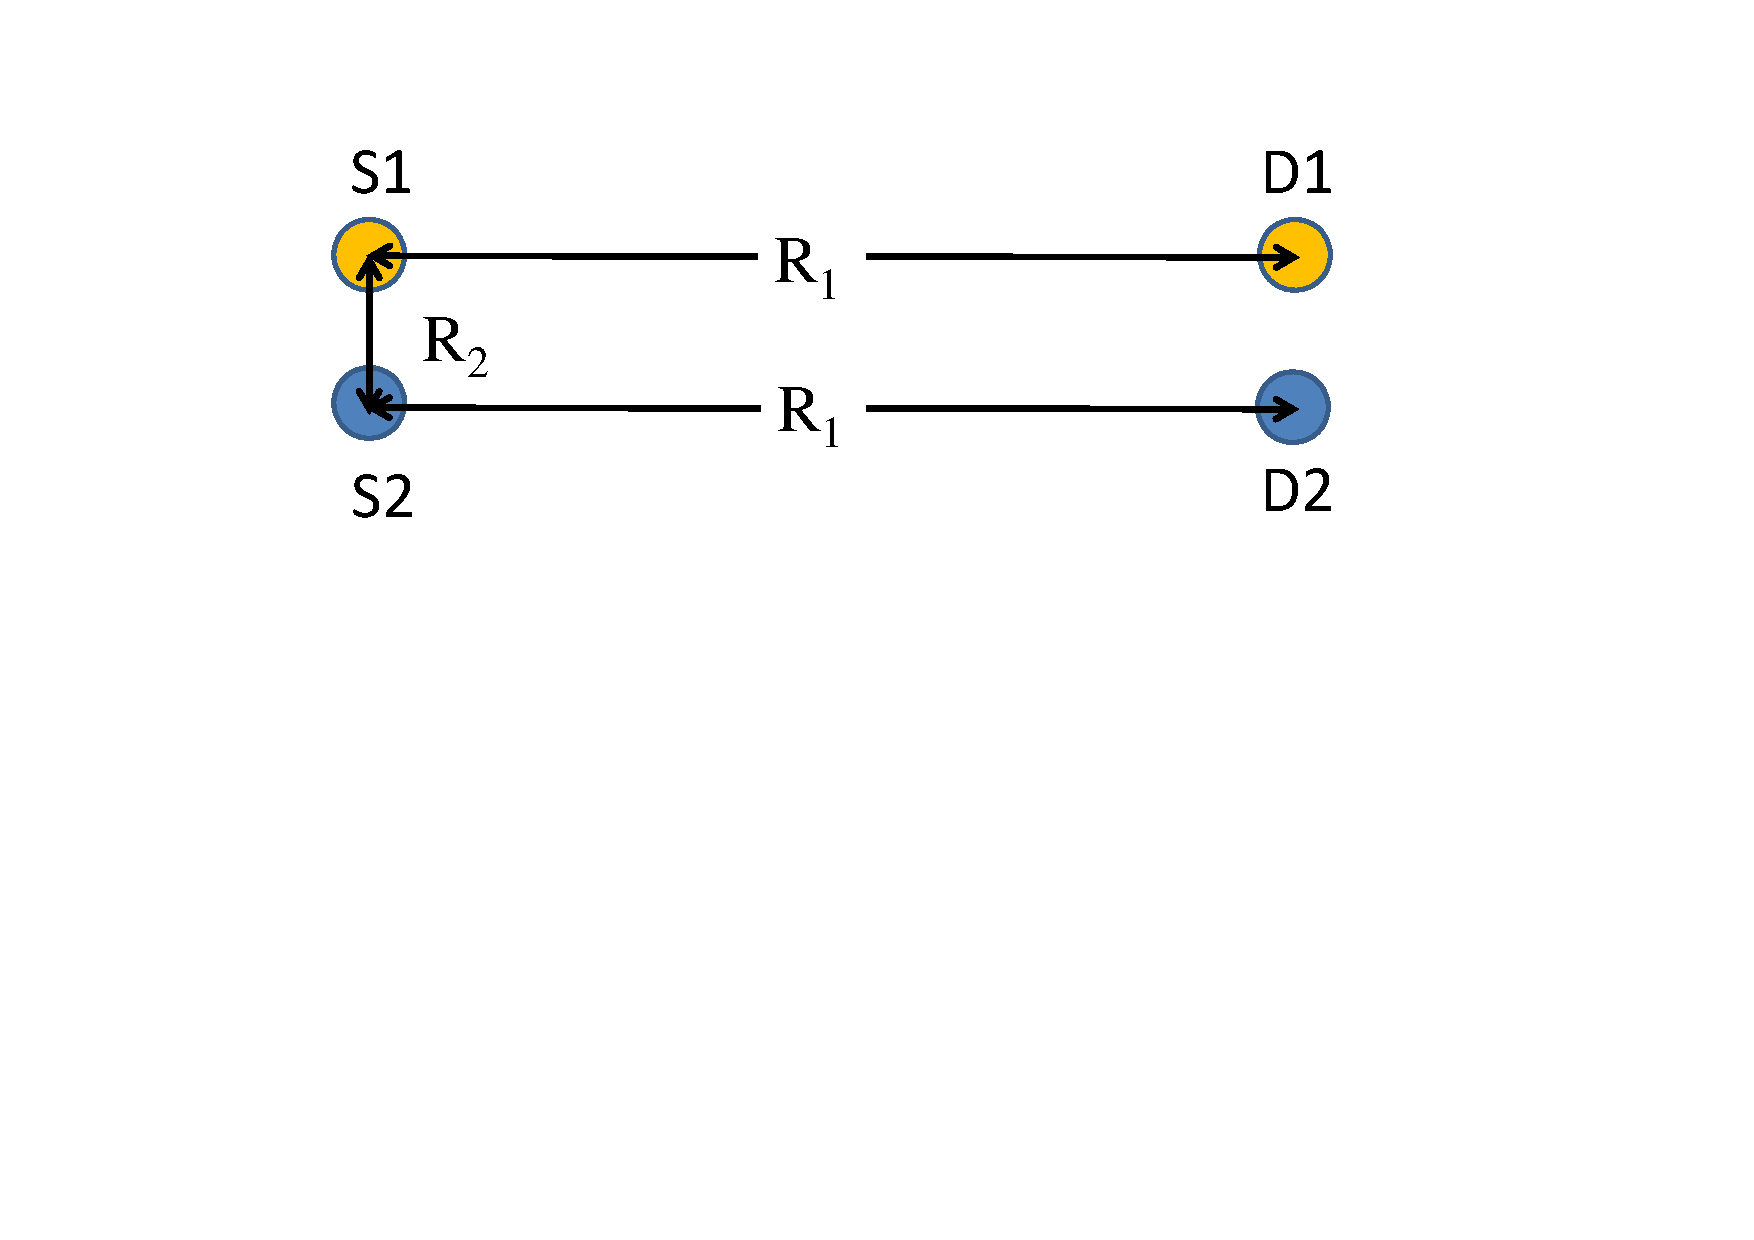
\includegraphics[width=160mm]{CompTestNodeAssignment.pdf}}
    \caption{Radio geometry for the competitive radio test. The distances are roughly $R_1 = 30$ feet and $R_2 = 3$ feet}
    \label{fig:CompTestNodeAssignment}
  \end{center}
\end{figure}

We assessed the performance of the competitive radio by running it with a pair of cooperative radios. The geometry of the set-up is shown in Figure~\ref{fig:CompTestNodeAssignment} with $R_1 = 30$ feet and $R_2 = 3$ feet. The cooperative radios are set up to transmit with a minimum number of sub-bands, which are selected as the sub-bands with the lowest energy level. Let the number of sub-bands to be used be denoted $N_{min}$. Test results are shown in Table \ref{tbl:COMPTestResultsStatic}. The metric is the amount of time (in seconds) for the competitive radio to successfully transmit 15000 packets.

In the DARPA Spectrum Challenge games, the software of our competitive radio crashed. Before it crashed, its performance was worse than some of other teams, namely Team Gator Wings and Team Wasabi \cite{DSCFinalEventResults}. Their radios occupied the same spectrum as ours, but their data could get through the interference while ours could not. 

\begin{table}[tpb]
\centering
    \caption{TEST RESULT (IN SECONDS): COMPETITIVE RADIO WITH COOPERATIVE RADIOS USING MINIMUM NUMBER OF SUB-BANDS (10 TESTS) \label{tbl:COMPTestResultsStatic}}
    \begin{tabular}{cccccc} \toprule
      {Test No.}
      &{No interference}
      &{$N_{min}=4$}
      &{$N_{min}=8$}
      &{$N_{min}=12$}  \\ \bottomrule
1	                  &33.4	&113.9	&192.7	&363.1 \\ \hline
2	                  &35.0	&136.0	&187.3	&360.5 \\ \hline
3	                  &34.1	&129.0	&189.2	&395.9 \\ \hline
4	                  &33.2	&133.3	&197.5	&363.2 \\ \hline
5	                  &33.2	&156.4	&227.2	&353.1 \\ \hline
6	                  &34.1	&136.7	&211.1	&331.5 \\ \hline
7	                  &34.0	&126.8	&206.1	&383.7 \\ \hline
8	                  &32.9	&120.5	&211.7	&362.9 \\ \hline
9	                  &33.5	&151.2	&189.3	&349.4 \\ \hline
10	                  &34.7	&139.3	&208.4	&284.0 \\ \bottomrule
Mean	              &33.8	&134.3	&202.0	&354.7 \\ \hline
Standard deviation	  &0.7	&12.9	&13.0	&30.5  \\ \bottomrule
    \end{tabular}
\end{table}

\section{Discussion}
\subsection{Observations from the Spectrum Challenge}
In the cooperative tournament, most teams utilized spectrum sensing, and a few teams performed real-time spectrum sensing. They continuously sensed even when they were transmitting on the source side. Their radios could shift almost immediately away from the spectrum where another team's signal suddenly appeared. Meanwhile, our radio sensed only once every 5 seconds and then transmitted on fixed sub-bands in one cooperative cycle. During our transmission, other teams could change their spectrum usage, resulting in spectrum conflicts.

In both competitive and cooperative games, our radio's power was less than that of many other teams' radios, even if they also used OFDM, which suggests that we still have room to optimize our power usage.

In the spectrum challenge, radios need to run on different USRPs, but the hardware of different USRPs is not exactly the same. Therefore, one parameter of the setup cannot maximize the power usage of all USRPs. Some teams calibrated their radios before a game started. For example, they would send a calibration signal sweeping across the 5 MHz bandwidth to find the best configuration of the transmission and receiving gains.

We also observed good synchronization between the transmitter and receiver. For example, Team MarmotE claimed their radios could achieve synchronization down to an SINR of -30 dB.

\subsection{Recommendations for Future Radio Design}
Real-time spectrum sensing should be developed to sense the spectrum all the time, and spectrum occupancy should be adjusted dynamically to avoid spectrum conflicts as the spectrum occupancy of other radios changes.

As discussed in the previous section, more work can be done to improve the synchronization of radios, to calibrate the radios and to increase the power usage of OFDM. Repetition codes can utilize time diversity as well as frequency diversity. The Fountain Code, Convolutional Code or Turbo Code could also be applied. The computational power of the PC is a bottleneck for channel coding because all of the signal processing is done in the PC. A PC is sufficient for a Repetition Code, Fountain Code, and Convolutional Code according to the observations of other teams as well as ours, but not for a Turbo Code. In the future, more sophisticated channel coding and signal processing techniques can be implemented in the FPGA of the USRP or a more capable SDR platform. In addition, a distributed spectrum access system with wider bandwidth can be explored.

The USRP N210 within the ORBIT testbed has two antennas. One antenna serves as a transceiver and the other is for reception only. Antenna diversity can be explored for a possible increase radio performance, as well.

Python is used for our packet management system, but we find Python has poor thread management. The threads in Python couple strongly with each other. One thread can significantly slow down the other one. In addition, as a scripting language, Python is much slower than C++. If a large amount of calculation is needed in limited time or multi-threading is necessary to deal with a significant workload, C++ is recommended instead of Python in GNU Radio.

Standard test tools and procedures should be developed for radio testing. When the radio designs are changed, the performance of radios should be measured and compared with the standards to determine if any improvement has been made. There should also be independent testers to test the radios, and developer should not responsible for the final test of their own radio components. Otherwise, errors and bugs are more likely to be hidden. A challenger is also very helpful. He or she can help the team find their weakness and look for solution to improve. During software development, good version control is also very important.

More extensively, an experiment design could be perused to determine parameters that could balance performance and robustness. Radio and network model for congested and interference-limited environment could be developed from such experimental data.


%
% Chapter 8
%

\chapter{CONCLUSION}
\label{chap:conclusion}
A cooperative distributed spectrum access system provides a way to share the spectrum without prior knowledge of other radios' information, such as modulation, bandwidth, signal amplitude, etc.. The number of wireless devices has been increasing dramatically while the spectrum resource is limited. The cooperative distributive spectrum access system provides another way to share the spectrum. It is also a potential solution to congested communication without prior coordination in severe conditions or extreme situations, such as natural disasters and accidents.

The competitive distributed spectrum access system provides a solution to deal with malicious radios using the same spectrum. It can automatically adjust its modulation and coding schemes according to the interference.

A packet management system is specially designed for the DARPA Spectrum Challenge. In the cooperative game, it can continue to provide packet service even if the reverse link is not reliable. Tests show that the packet management system has low cost while providing good feedback control.

This thesis also proposed a new spectrum sensing technique based on the statistical characteristics of the mean and the standard deviation of the interference signal energy across frequency. The spectrum sensing technique is analyzed and then implemented with GNU Radio and the USRP N210. Tests show that the technique can accurately detect the side lobes of the interference signal regardless of the signal level of the interference's signal.

A TDD system based on GNU Radio and the USRP N210 is also analyzed and implemented. Stream tags and burst control in GNU Radio and USRP are explored. The transition time between the forward and reverse link of the TDD system is within 200 $\mu s$. The implementation provides a good TDD example for the GNU Radio community.

Both the competitive radio and cooperative radio are good examples of the application of communication theory and practice. They could provide materials for a course focusing on radio implementation for congested or interference-limited environments. In this course, students will develop a good understanding of GNU Radio, the USRP, OFDM, spectrum sensing, TDD and related topics.

%
% Appendix (optional)
%

%\appendix

%
%%%%%%%%%%%%%%%%%%%%%%%%%%%%%%%%%%%%%%%%%%%%%%%%%%%%%%%%%%%%%%%%%%%%%%%%
%
% Appendix
%
%%%%%%%%%%%%%%%%%%%%%%%%%%%%%%%%%%%%%%%%%%%%%%%%%%%%%%%%%%%%%%%%%%%%%%%%

\chapter{CONCEPTS, AND DEFINITIONS}
This appendix provides a list of acronyms and abbreviations used throughout this dissertation, as well as simplified definitions of the most important concepts needed to understand the contents of
this dissertation.
\section{Acronyms and Abbreviations}
This section provides a list the acronyms and abbreviations used in this dissertation,
listed alphabetically.
\begin{itemize}

\item OFDM: Orthogonal Frequency Division Multiplexing

\item TDD: Time Division Duplex.

\end{itemize}

\section{Concepts and Terminology}
This section provides definitions of the most important concepts and terminology
needed to understand this dissertation, listed alphabetically by term, acronym,
or abbreviation.

\begin{itemize}
\item Destination node: The radio node that receives data packets over the air from the source node and send the received packets to the server.

\item Disable muter: Forward data samples from the USRP to next signal processing block.

\item Enable muter: Block the data samples from the USRP.

\item Forward link: Transmission from the source node to the destination.

\item Muter: A GNU radio block in the receiver that blocks the data from the USRP when current node is in the transmission state of a TDD cycle and that let the data from the USRP go through to next signal processing block when current node is in receiving state.

\item Packet: Data of 1400 bytes.

\item Physical-layer packet: packet that physical layer transmits in each subband.

\item Reverse link: Transmission from the destination node to the source.

\item Server: The server that sends data packet to the source node when requested by the source node and that receives and verifies the data packets sent from the destination node.

\item Source node: The radio node that requests data packets from the server and try to transmit them over the air.

\item Sub-packet: Packet that are pieces of the Packet in order to fit the physical-layer packet size requirement of the physical layer.

\item Tagger: A block that lies between the transmitter flow graph and the USRP in TDD mode, and that controls the burst transmission time in TDD mode.

\item TDD frame: The transmission period of a TDD cycle.

\item TDD sub-frame: A collection of Physical-layer packets that is synchronized by one group of preamble. Each sub-frame contains multiple physical-layer packets across the 5MHz frequency and during one TDD sub-frame, each OFDM tone only serves one Physical-layer packet.

\item Sub-frame left: a variable indicating how many sub frames are left in current TDD frame. Sub-frame left is contained in very physical-layer packet with one byte.
\end{itemize}


 % If you have appendices, add them here.
 % Begin each one with \chapter{TITLE} as before- the \appendix command takes
 % care of renaming chapter headings and creates a new page in the Table of
 % Contents for them.
 % \include{appendix-one}

\backmatter              % Place for bibliography and index


\bibliographystyle{nddiss2e}
\bibliography{Thesis}           % input the bib-database file name


\end{document}

%%
\endinput
%%
%% End of file `template.tex'.
